52\chapter{Results on \texorpdfstring{\PgU}{Y} production and suppression}
\label{chap:aupsilon}
\minitoc

\myepigraph{Life as a shorty shouldn’t be so rough.}{Inspectah Deck,
  in \textit{C.R.E.A.M.}, Wu-Tang Clan}


% CS1S_ppPt.pdf                  CS_AA_Rap_lin.pdf              RAA_RAP_Strickland_noAlice.pdf
% CS1S_ppPt_lin.pdf              RAA_NPART1S_Strickland.pdf     RAA_Rap-1.pdf
% CS1S_ppRap.pdf                 RAA_NPART_Rapp.pdf             RAA_nPart_4bins-1.pdf
% CS1S_ppRap_lin.pdf             RAA_NPART_Strickland.pdf       massPlot_PbPb_1Spp_equal.pdf
% CS_AAPt.pdf                    RAA_PT_Strickland.pdf          massPlot_PbPb_ppRAAscaled.pdf
% CS_AAPt_lin.pdf                RAA_Pt-1.pdf
% CS_AA_Rap.pdf                  RAA_RAP_Strickland_alice.pdf




In this Chapter, the information from Chapters~\ref{chap:ayield}
and~\ref{chap:aCorrection} is collected to produce the results of the
analysis of \PgU\ data in PbPb and $pp$ collisions. In the two cases, full
corrections $\acc\eff_{w}$ are applied to the raw yields. These corrected yields are
further normalised by the luminosity recorded in $pp$ in 2013 and by the number of minimum bias events in PbPb to get production rates. 

The cross section for \PgUa, \PgUb\ and \PgUc\ production in $pp$ collisions is presented
 in Section~\ref{sec:results_pp}.
Having the $pp$ spectra available for each state at this centre-of-mass
energy is a new and important addition to the already collected
quarkonium data. This, combined with the same measurement at other
centre-of-mass energies, can help towards a better understanding of quarkonium
production. % . These can be
% extended to measurements in different phase space ranges, such as the
% one performed by LHCb in~\cite{lhcbUpsi276}, or to other experiments
%such as the recent measurement done by ATLAS~\ref.

The PbPb spectra are presented in Section~\ref{sec:results_pbpb}, and represent a considerable
improvement with respect to~\cite{torsten}. The \PgUb\ spectrum is
 measured differentially for the first time in heavy ion collisions. It was discovered with the first heavy ion run of the
LHC in 2010 that \PgU\ states are suppressed in heavy ions, with
excited states being more suppressed than the \PgUa, as reported
in~\cite{torsten} and~\cite{HIN-11-007}. In the updated reference~\cite{11-011},
the centrality dependent result exhibits an ordering pattern, in
agreement with the sequential melting picture. 
The present study confirms this statement and allows to investigate its kinematical dependencies, thanks to the
twenty times larger statistics of the $pp$ reference. For example, it
becomes possible to check if the few surviving \PgUb\ would not be produced at high
\pt\ and escaping the plasma early on.  In the present Chapter,
updated measurements of the nuclear modification factor \RAA\ are
presented, differential in centrality, \pt\ and rapidity.%  double ratios which are presented 
% the emphasised on the
% centrality dependence of double ratios,  he PbPb data can be directly
% compared to $pp$ by the derivation of a nuclear modification factor
% for each state.

When a particle is not measurable with a good precision,
it can be more informative or more accurate to compute an upper limit
on the observed rate. This is what is done for the \PgUc, using a
fully frequentist statistical treatment of \PgUc\ yields from fits to
PbPb and $pp$ data, as presented in Section~\ref{sec:Y3S}. 

The results for \PgU\ suppression are compared to other experiments
and to theoretical models in Section~\ref{sec:comparisons}.

% To complete this review of the results, a few comparisons will be done.
\section{Measurement of the  \texorpdfstring{$pp$}{pp} cross section}
\label{sec:results_pp}
\subsection{Corrected yields}

First, let us collect the raw yields from Tables~\ref{tab:YieldsLoose} and~\ref{tab:YieldsTight}, and divide them
by their relative total corrections, \acc\eff$_{w}$ from Table~\ref{finalacceff_pp}. This 
gives an indication of the total number of events that have produced an \PgU\ in the rapidity range
$\vert\y\vert < 2.4$. The variations on signal extraction performed in Section~\ref{sec:sigext_vars} and reported in Tables~\ref{tab:systrecap1}
and~\ref{tab:systrecap2} are used to quote a systematic uncertainty on the total
number of \PgU. The corrected yields, statistical
and systematic uncertainties included, for \PgUa, \PgUb\ and \PgUc,
are presented in
Tables~\ref{tab:correctedyields1},~\ref{tab:correctedyields2}
and~\ref{tab:correctedyields3}, respectively. Each table contains the
results of the \pt-differential analysis, the rapidity differential
analysis, and the integrated result highlighted in bold font.

\begin{table}[h]
\begin{center}
\begin{tabular}{|c|c||c|c|}
\hline
\pt [\GeVc]& Total N[\PgUa](\pt)      & $\vert\y\vert$     &      Total N[\PgUa](\y) \\
% \hline
% 0.000-5.000     &0.357 $\pm$ 0.001   &  \\
% 5.000-12.000    & 0.309 $\pm$ 0.001  &  \\
% 12.000-20.000   & 0.513 $\pm$ 0.005  &  \\
\hline                                       
0-2.5             &4638 $\pm$ 157 $\pm$ 371  & 0-0.4   & 3642 $\pm$ 126 $\pm$ 109  \\
2.5-5             &6729 $\pm$ 217 $\pm$ 336  & 0.4-0.8 & 3774 $\pm$ 133 $\pm$ 113  \\
5-8               &4794 $\pm$ 162 $\pm$ 192  & 0.8-1.2 & 3286 $\pm$ 128 $\pm$ 131  \\
8-12              &2158 $\pm$ 99 $\pm$ 43    & 1.2-1.6 & 3180 $\pm$ 133 $\pm$ 127  \\
12-20             &838  $\pm$ 50 $\pm$ 8     & 1.6-2.0   & 2711 $\pm$ 141 $\pm$ 135  \\
\cline{1-2} 
\textbf{0-20}  &  \textbf{ 19137 $\pm$ 328 $\pm$ 628}  & 2.0-2.4  & 2957 $\pm$ 234 $\pm$ 236  \\
\hline                          
\end{tabular}
\caption{Corrected yields of \PgUa\ as a function of \pt\ and \y in
  $pp$ collisions at \s\ = 2.76 TeV. The left-hand side contains the results for the \pt-dependent binning. The right-hand side contains the results for the
  rapidity-dependent binning. On the left-hand side, the last entry at
the bottom (bold font) corresponds to the integrated result.}
\label{tab:correctedyields1}
\end{center}
\end{table}

% From the \pt\-binned results, one can check that the sum of yields agrees with the integrated result, which is actually true at the level of 0.1\%. 

It is to be noted that the systematic uncertainty from fitting decreases significantly with \pt, which is due to the background level dropping, making the remaining signal easier to fit. 

% From the rapidity-binned results, one can sum the yields to a slightly larger number than the integrated result: this is understood by the upper \pt\ bound at 20~\GeVc not being applied when binning in rapidity.

%  Above this limit, we have considered that there are too few
% events in PbPb, so a higher-\pt\ bin such as the one presented in
% Figure~\ref{fig:extrabin} on is not included in
% the final result. However, there are good reasons to think that a
% further iteration of this analysis, using Run 2 PbPb and $pp$ data at
% for the suppression of excited states.

\begin{table}[h]
\begin{center}
\begin{tabular}{|c|c||c|c|}
\hline
\pt [\GeVc]& Total N[\PgUb](\pt)      & $\vert\y\vert$     &    Total N[\PgUb](\y) \\
% \hline
% 0.000-5.000     &0.357 $\pm$ 0.001   &  \\
% 5.000-12.000    & 0.309 $\pm$ 0.001  &  \\
% 12.000-20.000   & 0.513 $\pm$ 0.005  &  \\
\hline                                       
0-2.5             &1022 $\pm$ 99  $\pm$ 112 & 0-0.4   &1046 $\pm$ 82 $\pm$ 52    \\
2.5-5             &1483 $\pm$ 140 $\pm$ 59  & 0.4-0.8 &1031 $\pm$ 84 $\pm$ 52    \\
5-8               &1431 $\pm$ 118 $\pm$ 57  & 0.8-1.2 &962  $\pm$ 87 $\pm$ 87    \\
8-12              &801  $\pm$ 72  $\pm$ 24  & 1.2-1.6 &974  $\pm$ 94 $\pm$ 88    \\
12-20             &313  $\pm$ 34  $\pm$ 3   & 1.6-2.0   &924  $\pm$ 102 $\pm$ 129  \\
\cline{1-2} 
\textbf{0-20}  &  \textbf{5541 $\pm$ 225 $\pm$ 116}  & 2.0-2.4  &  634  $\pm$ 166 $\pm$ 19 \\
\hline                          
\end{tabular}
\caption{Corrected yields of \PgUb\ as a function of \pt\ and \y in $pp$ collisions at \s\ = 2.76 TeV. Same conventions as Table~\ref{tab:correctedyields1}.}
\label{tab:correctedyields2}
\end{center}
\end{table}


\begin{table}[h]
\begin{center}
\begin{tabular}{|c|c||c|c|}
\hline
\pt [\GeVc]& Total N[\PgUc](\pt)      & $\vert\y\vert$     &    Total N[\PgUc](\y) \\
% \hline
% 0.000-5.000     &0.357 $\pm$ 0.001   &  \\
% 5.000-12.000    & 0.309 $\pm$ 0.001  &  \\
% 12.000-20.000   & 0.513 $\pm$ 0.005  &  \\
\hline                                       
0-2.5             &362 $\pm$ 67 $\pm$ 54 & 0-0.4   & 431 $\pm$ 54 $\pm$ 30  \\
2.5-5             &775 $\pm$ 102 $\pm$ 39 & 0.4-0.8 & 422 $\pm$ 57 $\pm$ 30  \\
5-8               &570 $\pm$ 82 $\pm$ 28 & 0.8-1.2 & 465 $\pm$ 62 $\pm$ 51  \\
8-12              &338 $\pm$ 51 $\pm$ 13 & 1.2-1.6 & 360 $\pm$ 66 $\pm$ 36  \\
12-20             &178 $\pm$ 27 $\pm$ 3  & 1.6-2.0   & 340 $\pm$ 71 $\pm$ 20  \\
\cline{1-2} 
\textbf{0-20}  &  \textbf{2353 $\pm$ 156 $\pm$ 71}  &2-2.4  &559 $\pm$ 137 $\pm$ 17   \\
\hline                          
\end{tabular}
\caption{Corrected yields of \PgUc\ as a function of \pt\ and \y in $pp$ collisions at \s\ = 2.76 TeV. Same conventions as Table~\ref{tab:correctedyields1}.}
\label{tab:correctedyields3}
\end{center}
\end{table}
% \vfill~\\                       


\subsection{Differential cross sections}

The differential cross sections for \PgU(nS) production in $pp$ are defined as
the fraction of \PgU(nS) events measured in a given bin, corrected for
acceptance and efficiency (including the tag and probe efficiency
corrections), normalised with $\mathcal{L}_{pp}$, the luminosity
of the $pp$ sample, and divided by the width of the bin considered. Since the analysis is
single differential in \pt\ and rapidity, one can define a
\pt-differential and a rapidity-differential cross section, namely:

\begin{eqnarray} 
\label{eq:cspt}
\dfrac{1}{\Delta y}\ \dfrac{\text{d}\sigma\left( pp\rightarrow
    \PgU(nS)X\right)}{\text{d}\pt} \cdot B_{\mu\mu} &=&
\dfrac{1}{\Delta y \Delta
  \pt}\cdot\dfrac{1}{\mathcal{L}_{pp}}\cdot\dfrac{\NFitnS}{\alpha\
  \eff_{pp, w} } \\
\label{eq:csrap}
\dfrac{\text{d}\sigma\left( pp\rightarrow
\PgU(nS)X\right)}{\text{d}y} \cdot B_{\mu\mu} &=&
\dfrac{1}{\Delta
  y}\cdot\dfrac{1}{\mathcal{L}_{pp}}\cdot\dfrac{\NFitnS} {\alpha\
  \eff_{pp, w}} 
\end{eqnarray}
% 
where:
\begin{itemize}
\item[-]{\NFitnS\ is the number of measured $\PgU$(nS) decaying to
two muons, extracted from the fit
to data in Section~\ref{sec:sigext},}
\item[-]{$\alpha$ is the geometric acceptance, computed in Section
\ref{sec:acceptance},}
\item[-]{$\varepsilon_{pp, w}$ is the dimuon detection efficiency, weighted with its own
    tag and probe corrections,}
\item[-]{$\mathcal{L}_{pp}$ = (5.4 $\pm$ 0.2) pb$^{-1}$ is the integrated
luminosity of the $pp$ sample,}
\item[-]{$\Delta\pt$ and $\Delta\y$ are the bin widths in $\pt$ and $y$,
    as described in Section~\ref{sec:sigext_yield}.
    In Equation~\ref{eq:cspt} as well as in Tables~\ref{tab:correctedyields1},~\ref{tab:correctedyields3}
    and~\ref{tab:correctedyields3}, the \pt-binned cross sections are divided by $\Delta\y = 4.8$ to ease the comparison
    with other experiments,}
\item[-]{$B_{\mu\mu}$ is the branching fraction of each \PgU\ state into
    its dimuon decay. It is implicit in the result, and is not used in
    the present calculation.}
\end{itemize}
%
The $pp$ cross sections are shown as
a function of \pt\ in Figure~\ref{fig:ppCrossSections_pt} and as a function of
\y\ in Figure~\ref{fig:ppCrossSections_y}. Tabulated results for \PgUa,
\PgUb\ and \PgUc\ are reported in Tables~\ref{tab:CSpp_tab1},~\ref{tab:CSpp_tab2}
    and~\ref{tab:CSpp_tab3}, respectively.
%\vfill\newpage
%
\begin{figure}
\begin{centering}  
  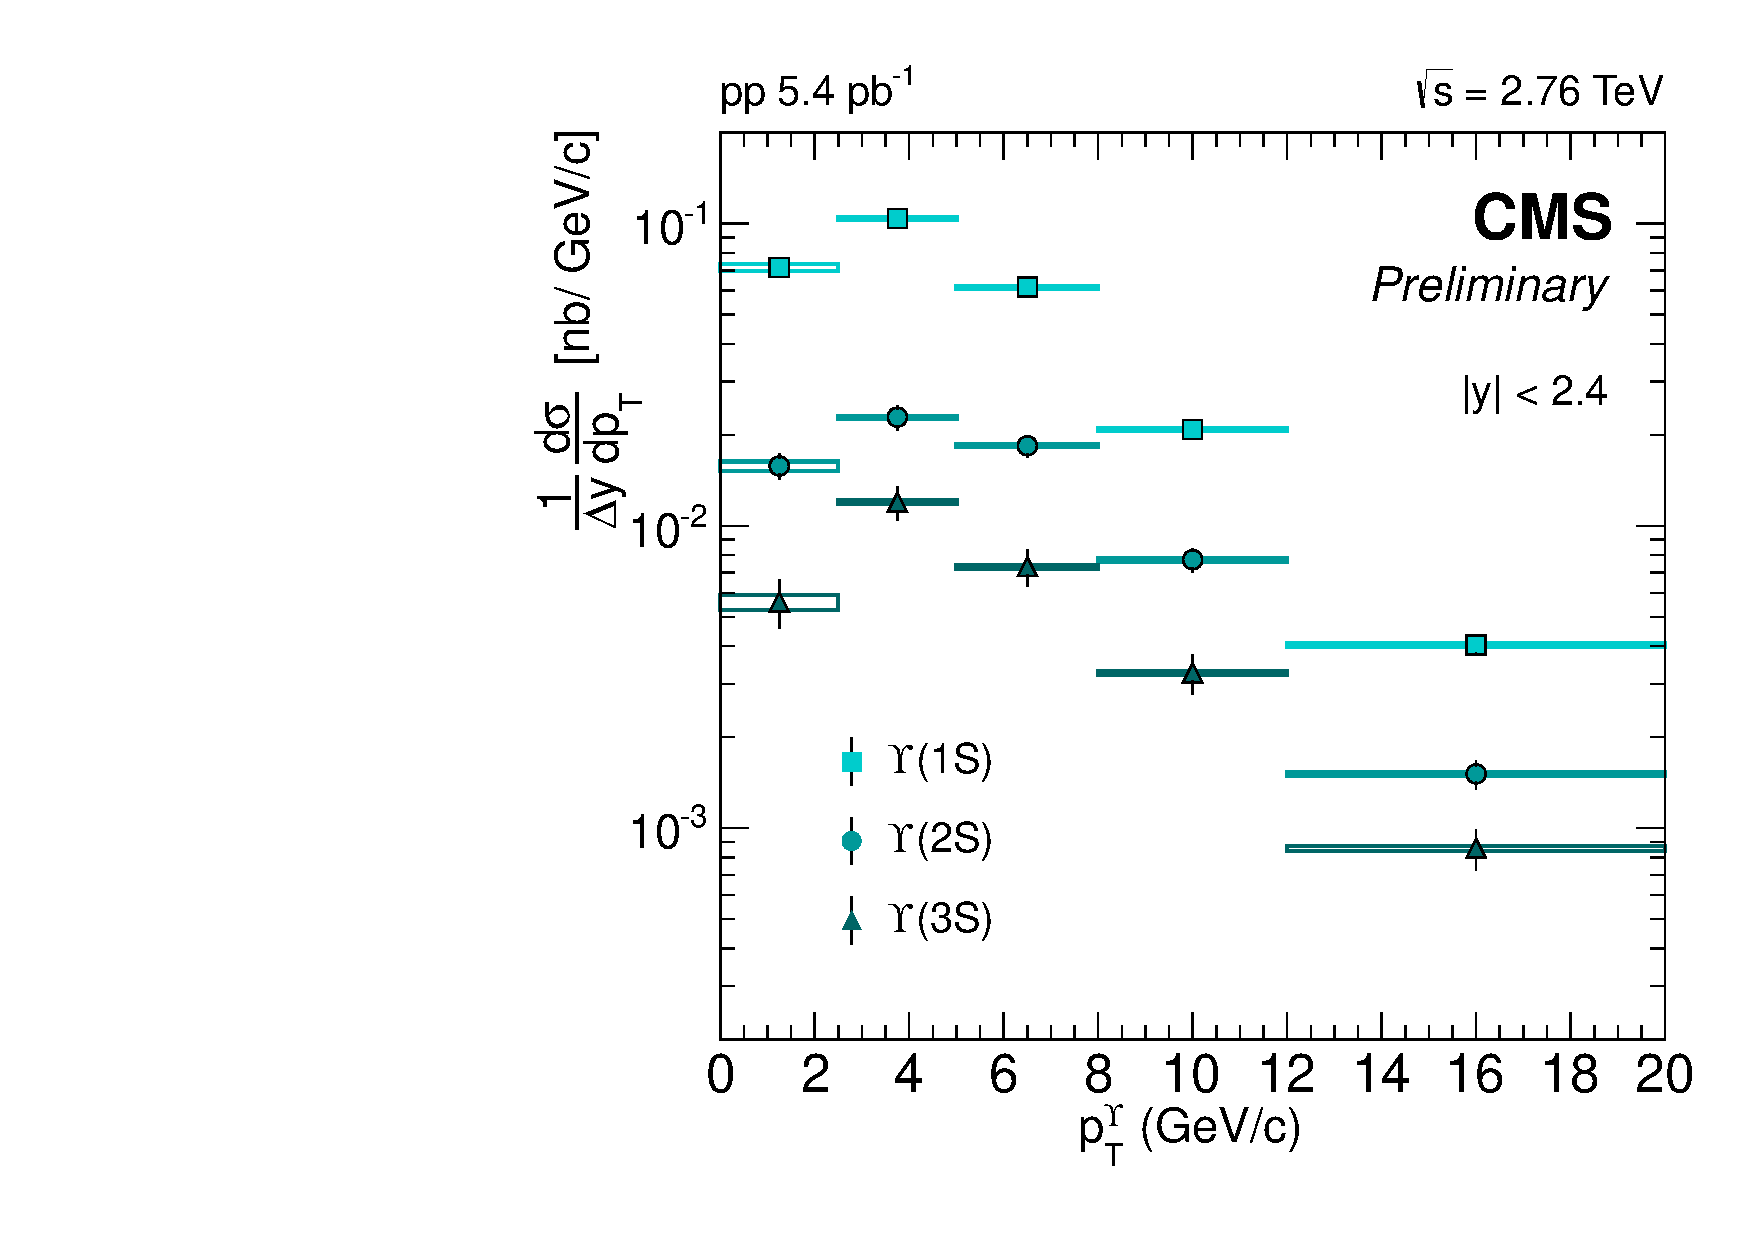
\includegraphics[width=0.69\textwidth]{Chapters/aUpsilon/CS1S_ppPt.pdf}
%  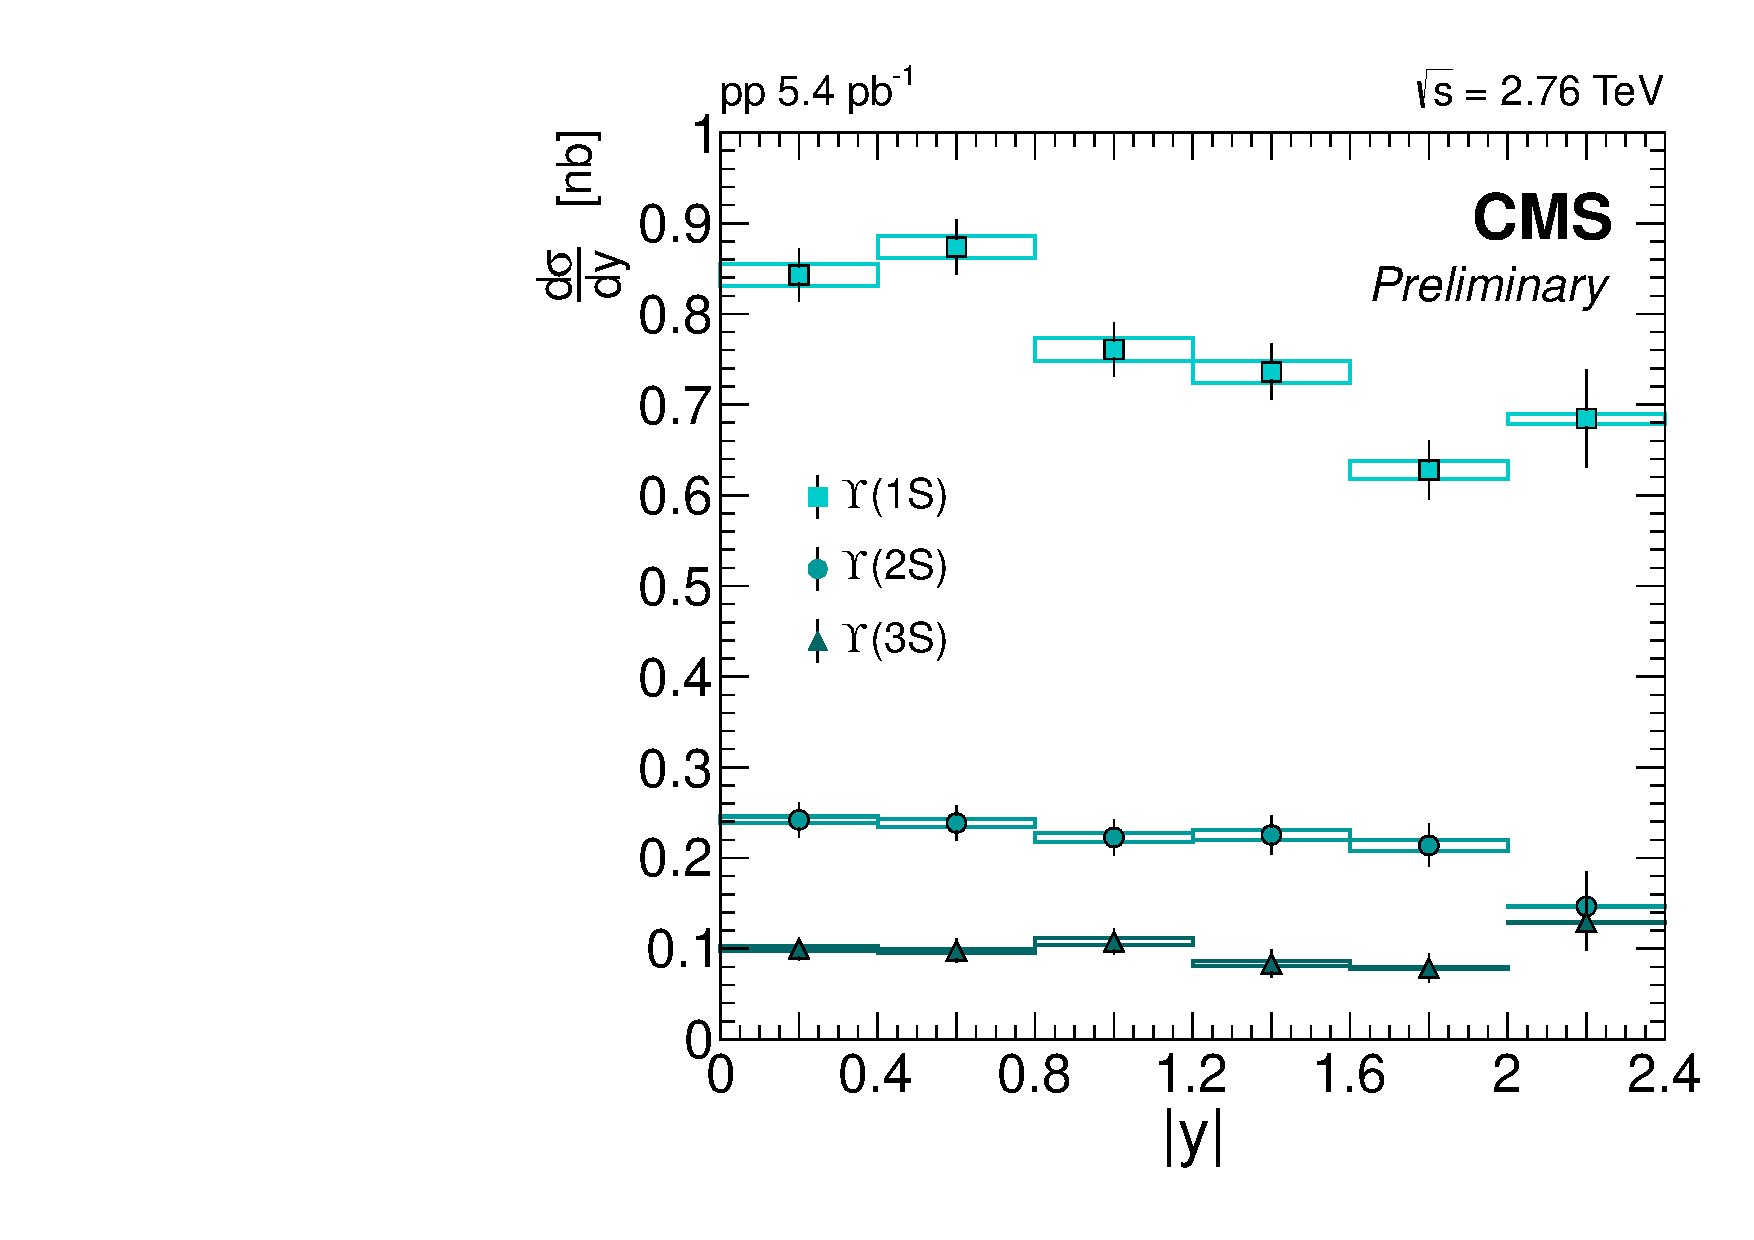
\includegraphics[width=0.49\textwidth]{Chapters/aUpsilon/CS1S_ppRap_lin.pdf}
  \caption{Cross sections for $pp \to \PgU(nS) \to \mu\mu$ in $\vert\y\vert < 2.4$, as a function of the \PgU\ transverse
    momentum. A global systematic uncertainty (luminosity, tracking efficiency) of 5\% is not displayed.}
  \label{fig:ppCrossSections_pt}
\end{centering}  
\end{figure}
\begin{figure}
\begin{centering}  
 % 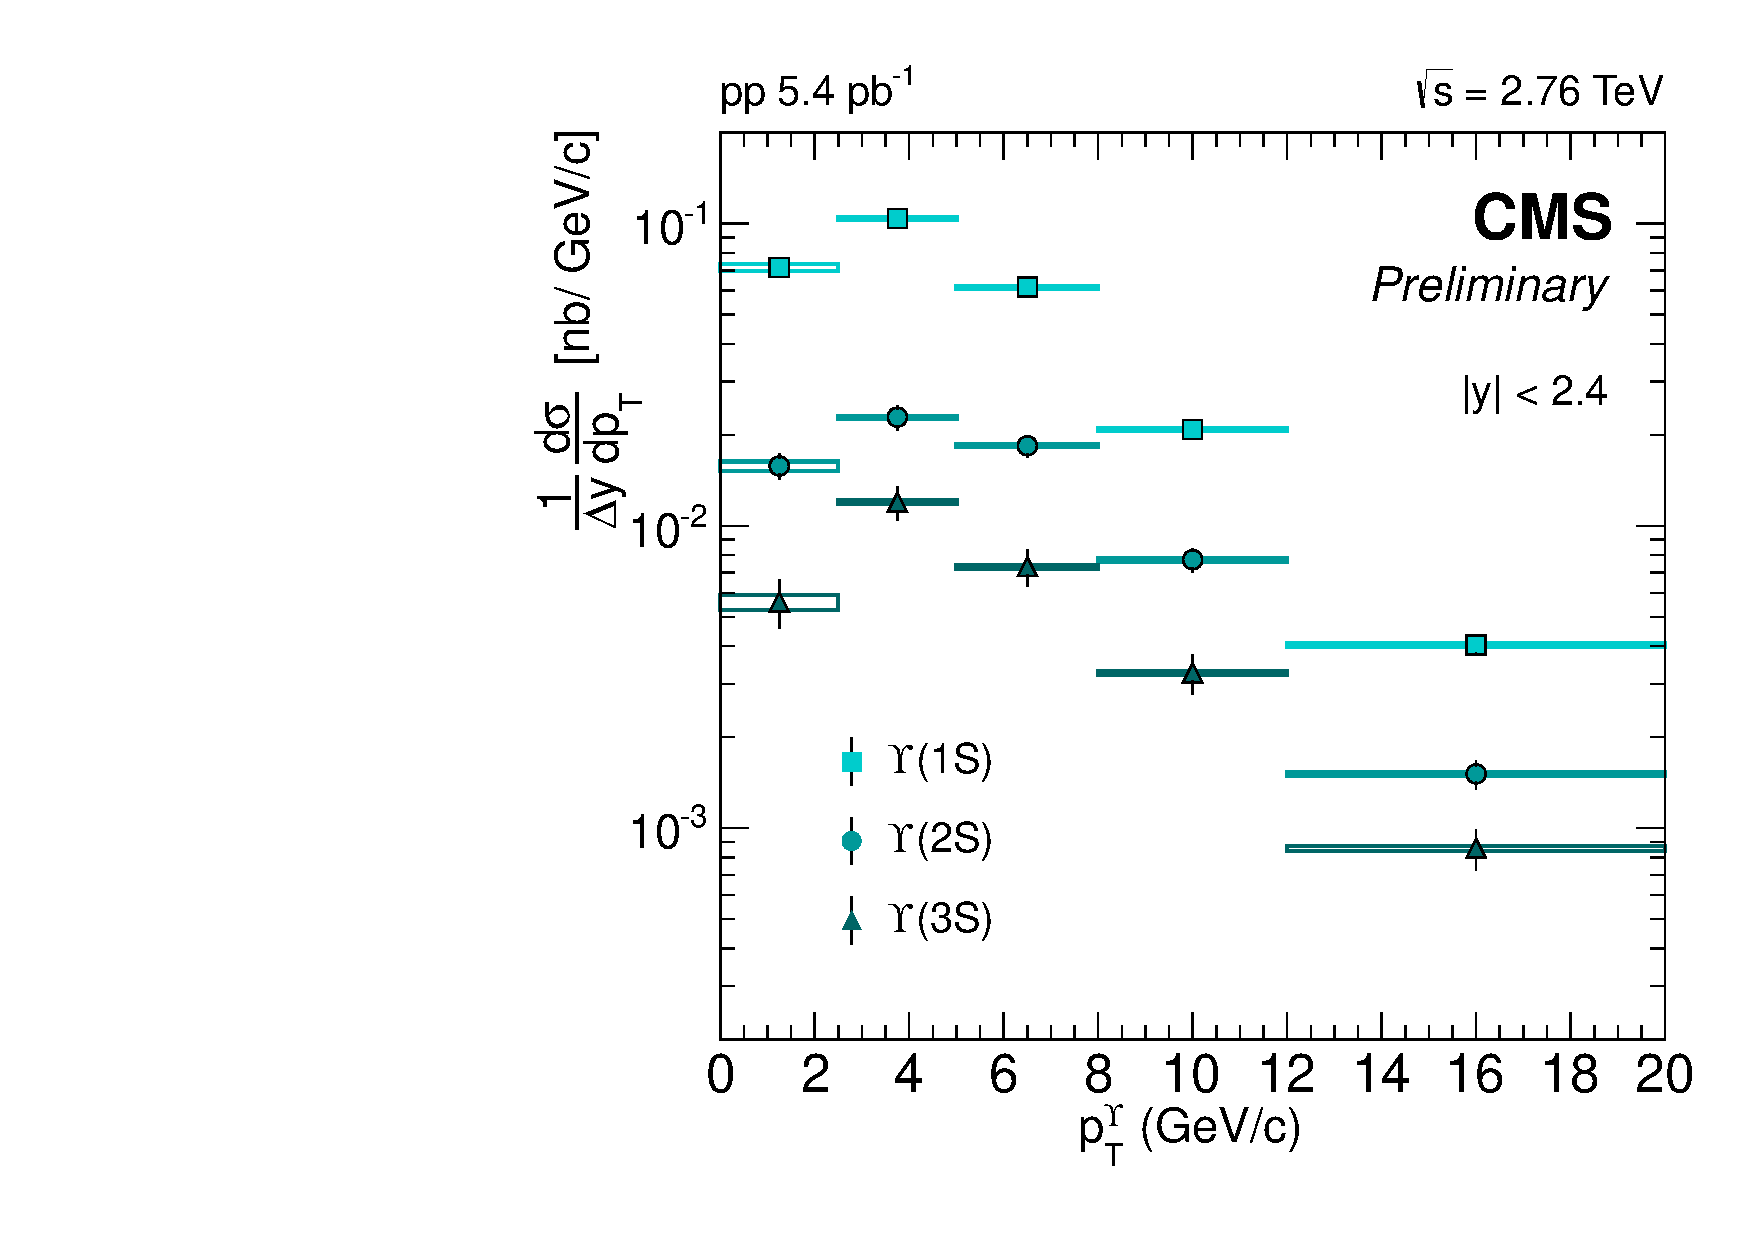
\includegraphics[width=0.49\textwidth]{Chapters/aUpsilon/CS1S_ppPt.pdf}
  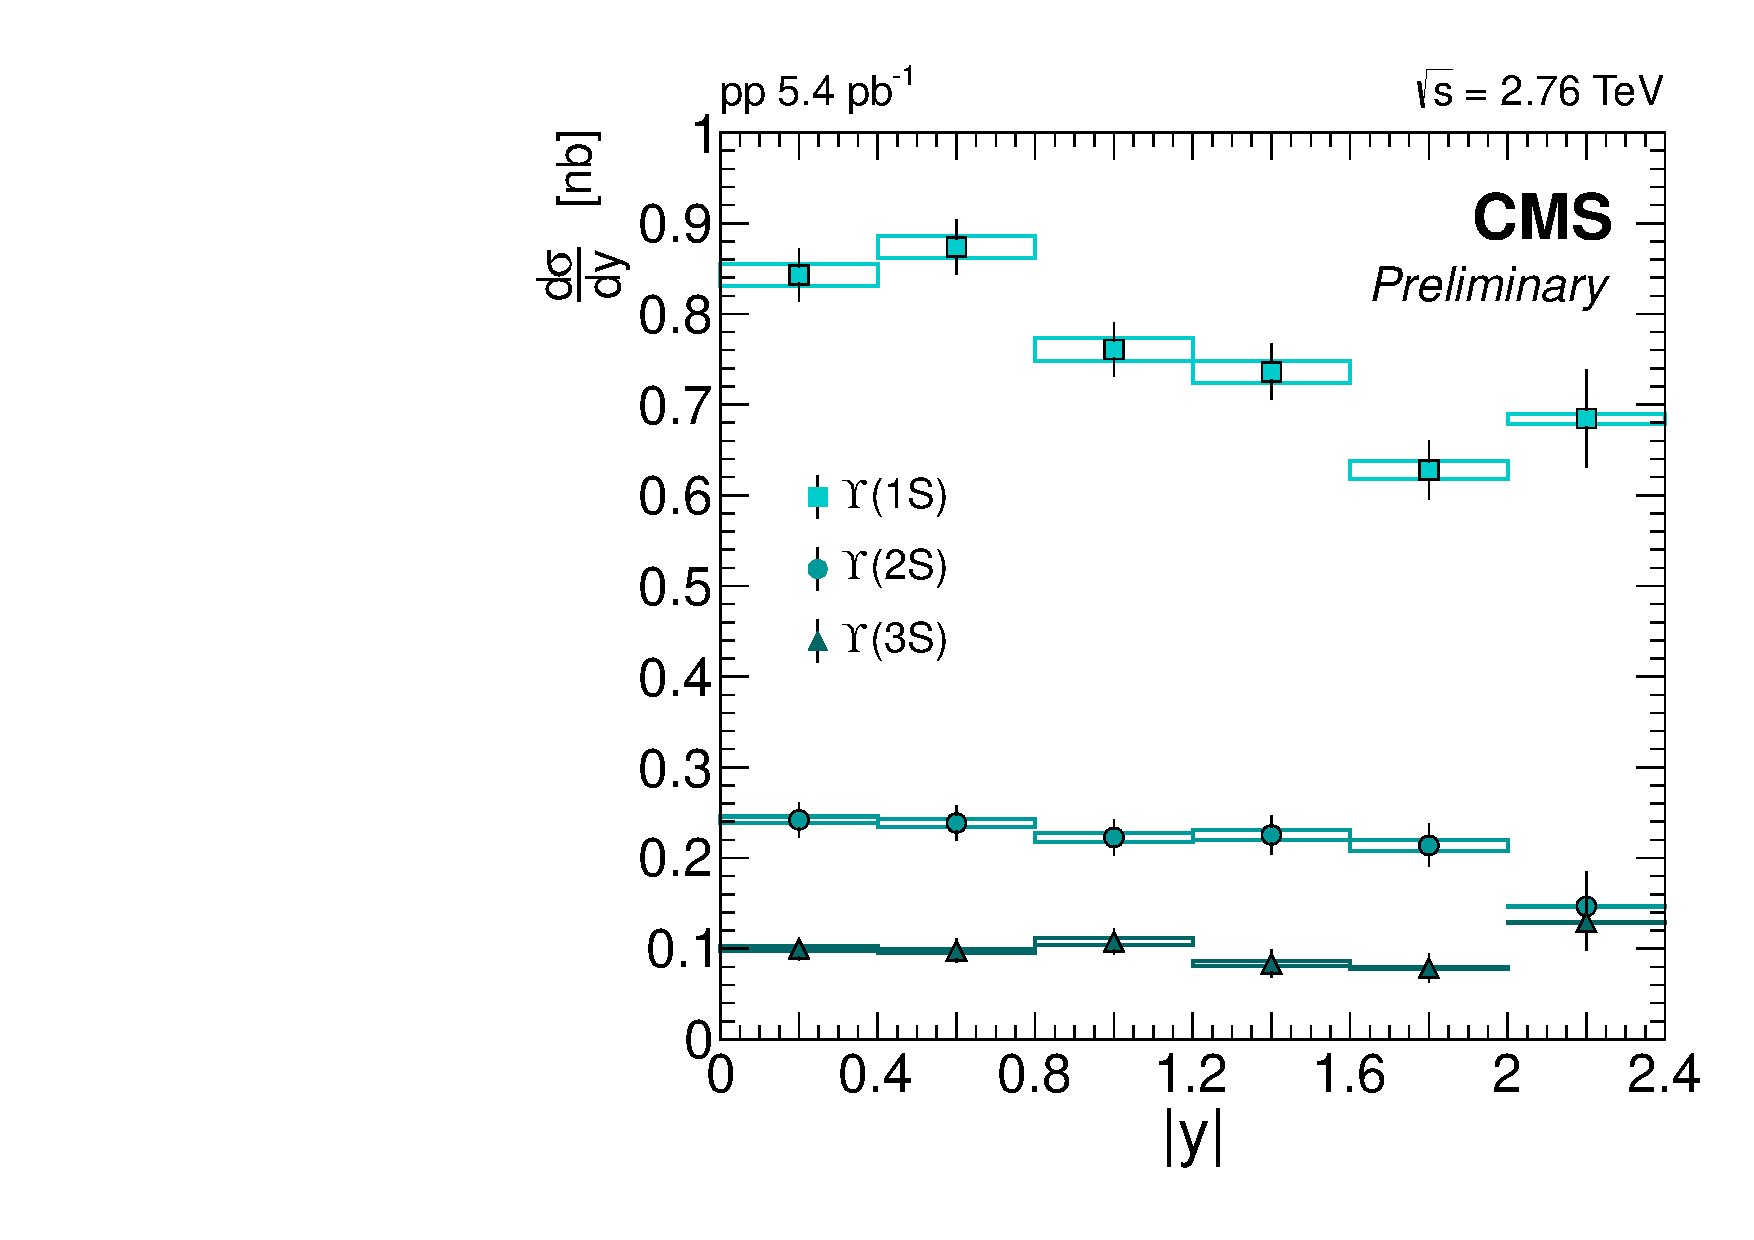
\includegraphics[width=0.69\textwidth]{Chapters/aUpsilon/CS1S_ppRap_lin.pdf}
  \caption{Cross sections for $pp \to \PgU(nS) \to \mu\mu$ in $\vert\y\vert < 2.4$, as a function of the \PgU\ rapidity. A global luminosity uncertainty (luminosity, tracking efficiency) of 5\% is not displayed.}
  \label{fig:ppCrossSections_y}
\end{centering}  
\end{figure}


\begin{table}[h]
\begin{center}
\begin{tabular}{|c|c||c|c|}
\hline
\pt [\GeVc]& $\frac{1}{\Delta y}\frac{d\sigma(\PgUa)}{d\pt}\cdot B_{\mu\mu}$ [nb $\cdot$ c/GeV]      & $\vert\y\vert$     &  $\frac{d\sigma(\PgUa)}{d\y}\cdot B_{\mu\mu}$ [nb]\\
\hline                                       
0-2.5             &  0.073 $\pm$ 0.0025 $\pm$ 0.0020   & 0-0.4       & 0.881 $\pm$ 0.031 $\pm$ 0.012  \\
2.5-5             &  0.105 $\pm$ 0.0034 $\pm$ 0.0014   & 0.4-0.8     & 0.910 $\pm$ 0.032 $\pm$ 0.012    \\
5-8               &  0.062 $\pm$ 0.0021 $\pm$ 0.0006   & 0.8-1.2     & 0.789 $\pm$ 0.031 $\pm$ 0.012  \\
8-12              &  0.021 $\pm$ 0.0009 $\pm$ 0.0002   & 1.2-1.6     & 0.762 $\pm$ 0.032 $\pm$ 0.012  \\
12-20             &  0.0041 $\pm$ 0.0002 $\pm$ 6$\cdot10^{-5}$ &1.6-2.0 & 0.644 $\pm$ 0.034 $\pm$ 0.010 \\
\cline{1-2}
\textbf{0-20}  &  \textbf{3.544 $\pm$ 0.067 $\pm$ 0.109}  & 2.0-2.4  &   0.710 $\pm$ 0.056 $\pm$ 0.006   \\                         
\hline                          
\end{tabular}
\caption{\PgUa\ differential cross sections in  $pp$ collisions as a
  function of \pt\ and \y. Same conventions as Table~\ref{tab:correctedyields1}, with the exception that the integrated cross section, lower left line, is note divided by $\Delta y$.}
\label{tab:CSpp_tab1}
\end{center}
\end{table}

\begin{table}[h]
\begin{center}
\begin{tabular}{|c|c||c|c|}
\hline
\pt [\GeVc]& $\frac{1}{\Delta y}\frac{d\sigma(\PgUb)}{d\pt}\cdot B_{\mu\mu}$ [nb $\cdot$ c/GeV]      & $\vert\y\vert$     &  $\frac{d\sigma(\PgUb)}{d\y}\cdot B_{\mu\mu}$ [nb]\\

\hline                                       
0-2.5             &0.0158 $\pm$ 0.0015 $\pm$ 0.0006  & 0-0.4       & 0.242 $\pm$ 0.019 $\pm$ 0.004   \\
2.5-5             &0.0229 $\pm$ 0.0021 $\pm$ 0.0002  & 0.4-0.8     & 0.239 $\pm$ 0.019 $\pm$ 0.004    \\
5-8               &0.0184 $\pm$ 0.0015 $\pm$ 0.0002  & 0.8-1.2     & 0.223 $\pm$ 0.020 $\pm$ 0.005   \\
8-12              &0.0077 $\pm$ 0.0007 $\pm$ 0.0001  & 1.2-1.6     & 0.225 $\pm$ 0.022 $\pm$ 0.005   \\
12-20             &0.0015 $\pm$ 0.0002 $\pm$ 2$\cdot 10^{-5}$  & 1.6-2.0       & 0.214 $\pm$ 0.024 $\pm$ 0.006  \\
\cline{1-2}
\textbf{0-20}  &  \textbf{1.026 $\pm$ 0.042 $\pm$ 0.037}  & 2.0-2.4 & 0.147 $\pm$ 0.038 $\pm$ 0.001     \\                         
\hline                          
\end{tabular}
\caption{\PgUb\ differential cross sections in  $pp$ collisions as a
  function of \pt\ and \y. Same conventions as Table~\ref{tab:CSpp_tab1}.}
\label{tab:CSpp_tab2}
\end{center}
\end{table}

\begin{table}[h]
\begin{center}
\begin{tabular}{|c|c||c|c|}
\hline
\pt [\GeVc]& $\frac{1}{\Delta y}\frac{d\sigma(\PgUc)}{d\pt}\cdot
B_{\mu\mu}$ [nb $\cdot$ c/GeV]      & $\vert\y\vert$     &
$\frac{d\sigma(\PgUc)}{d\y}\cdot B_{\mu\mu}$ [nb] \\
\hline                                       
0-2.5             & 0.0056 $\pm$ 0.0010 $\pm$ 0.0003  & 0-0.4         & 0.100 $\pm$ 0.013 $\pm$ 0.003   \\
2.5-5             & 0.0120 $\pm$ 0.0016 $\pm$ 0.0001  & 0.4-0.8       & 0.098 $\pm$ 0.013 $\pm$ 0.002    \\
5-8               & 0.0073 $\pm$ 0.0010 $\pm$ 0.0001  & 0.8-1.2       & 0.108 $\pm$ 0.014 $\pm$ 0.004    \\
8-12              & 0.0033 $\pm$ 0.0005 $\pm$ 5$\cdot10^{-5}$ & 1.2-1.6& 0.083 $\pm$ 0.015 $\pm$ 0.003   \\
12-20             & 0.0008 $\pm$ 0.0001 $\pm$ 1$\cdot10^{-5}$ & 1.6-2.0  & 0.079 $\pm$ 0.016 $\pm$ 0.001  \\
\cline{1-2}
\textbf{0-20}  &  \textbf{0.436 $\pm$ 0.029 $\pm$ 0.008} & 2.0-2.4 & 0.129 $\pm$ 0.032 $\pm$ 0.001 \\
\hline                          
\end{tabular}
\caption{\PgUc\ differential cross sections in  $pp$ collisions as a
  function of \pt\ and \y. Same conventions as Table~\ref{tab:CSpp_tab1}.}
\label{tab:CSpp_tab3}
\end{center}
\end{table}


The $pp$ cross sections are presented with systematic uncertainties,
which are computed as the quadratic sum of the following
contributions:
\begin{itemize}
\item[-] The fitting uncertainty from Section~\ref{sec:sigext_vars}:
  This source of uncertainty 
  decreases continuously with the amount of background under the
  peak, when increasing the \pt\ range considered. The first \pt\ bin,
  $\pt < 2.5~\GeVc$ has systematic uncertainties of 8\%, 11\%, 15\% for \PgUa, \PgUb\
  and \PgUc, respectively,
\item[-] The generated spectrum assumed by PYTHIA, as seen in
  Section~\ref{sec:acceff_syst} ranging around 2-3\%.
\item[-] The tag and probe single muon
  efficiencies, computed in Section~\ref{sec:tnp}, whose effect
  on the dimuon efficiency has been assigned a systematic uncertainty
  in Section~\ref{sec:tnp_syst}. The size of the uncertainty (2-15\%) depends
  on the collision setup ($pp$, PbPb) and the region of phase space
  (\pt, $\eta$) studied.
\end{itemize}

Additionally, global uncertainties (affecting all points together) are
computed to be 5\% in $pp$, and are not shown in the
Figures~\ref{fig:ppCrossSections_pt} and~\ref{fig:ppCrossSections_y}. The luminosity $\mathcal{L}_{pp}$
is known to the 3.7\% accuracy. The tracking efficiency in $pp$
adds another source of systematic uncertainty of 1.7\% per
muon.
\vspace{0.3cm}

\fbox{
  \parbox{0.9\textwidth}
  {\textsf{In this section, we have seen that the LHC has provided almost
      twenty thousand \PgUa, more than five thousand \PgUb, and two thousand
      \PgUc\ decaying in two muons in the CMS detector during its running time in 2013, with $pp$
      collisions at the centre-of-mass energy of \s~= 2.76 \TeV. These were
      produced when accumulating a luminosity of  $\mathcal{L}_{pp}$ = (5.4 $\pm$ 0.2)
      \invpb. The integrated cross sections $\sigma(pp \to \PgU(nS)
      X)\cdot B_{\mu\mu}$ measured in $\vert\y\vert < 2.4$, are: 
      \begin{eqnarray*}
        \sigma\left(pp \to \PgUa X \right)  \cdot  B_{\mu\mu} &=& 3.544 \pm 0.067 \pm 0.109~\textrm{nb} \\
        \sigma\left(pp \to \PgUb X \right) \cdot B_{\mu\mu} &=& 1.026 \pm 0.042 \pm  0.037~\textrm{nb} \\
        \sigma\left(pp \to \PgUc X \right) \cdot B_{\mu\mu} &=& 0.436 \pm
        0.029 \pm 0.008~\textrm{nb} .
      \end{eqnarray*}
      In the following section, we will see how this compares to the
      observed \PgU\ yields in PbPb collisions.}}
}


% These can be further compared to equivalent measurements at other
% energies and in different regions of the phase space, to get a better
% understanding of the 
%discussion of the systematic uncertainties


%\subsection{Comparisons with models and experiments}
%comparisons to other experiments

%comparisons with models? RAMONA

%sqrt{s} dependence?
\newpage
\section{\texorpdfstring{\PgU}{Y} suppression in heavy ion collisions}
\label{sec:results_pbpb}
\subsection{Normalised cross sections}

\label{subsec:csaa}
% The \PgU\ mesons produced in heavy ion experiments need to be
% normalised to a proper number accounting for the luminosity of the
% recorded sample. This number is the product of the number of minimum
% bias events, \NMB, and the nuclear overlap function \TAA, integrated
% over 
The differential \PgU\ yield is corrected for acceptance and tag and
probe weighted efficiencies, and further normalised by the product of
\NMB\ and \TAA, the normalisation factors for heavy ion experiments
already encountered in Chapter~\ref{chap:xmuons}.%  The following
% expressions are used to compare directly with $pp$ cross sections as
% they are taking into account \TAA, the nuclear overlap function, that
% encapsulates how nucleons are distributed in the interacting nuclei. In other words, dividing by \TAA brings the yield to the nucleon-nucleon level and gives it the units of a cross section. 

Equation~\ref{eq:nypt} shows the \TAA-scaled corrected \PgU(nS) yields
as a function of \pt, and Equation~\ref{eq:nyrap}
as a function of rapidity:
%computed via the following Equations \ref{eq:nypt} and \ref{eq:nyrap}
%for $\pt$ and $y$ dependence, respectively:
\begin{eqnarray} 
\label{eq:nypt}
% \YPbPb(\pt) \equiv
\dfrac{1}{\TAA} \cdot \dfrac{1}{\Delta y} \cdot \dfrac{\text{d}N\left( AA\rightarrow
 \PgU(nS)\right)}{\text{d}\pt} \cdot B_{\mu\mu} &=&
 \dfrac{1}{\TAA}\cdot
 \dfrac{1}{\NMB}\cdot\dfrac{\NFitnSPbPb}{\alpha\ \varepsilon_{\rm PbPb}\
 \Delta \pt\Delta y}, \\
\label{eq:nyrap}
% \YPbPb(y) \equiv 
\dfrac{1}{\TAA} \cdot \dfrac{\text{d}N\left( AA\rightarrow
 \PgU(nS)\right)}{\text{d}y} \cdot B_{\mu\mu} &=&
 \dfrac{1}{\TAA} \cdot
  \dfrac{1}{\NMB} \cdot \dfrac{\NFitnSPbPb}{\alpha\ \varepsilon_{\rm PbPb}\ \Delta y}, 
 \end{eqnarray}    
% 
where
\begin{itemize}
\item{\NFitnSPbPb\ is the number of measured \PgU(nS) decaying to
    two muons, from the fit
    to data in Section~\ref{sec:sigext_fits};}
\item{$\alpha$ is the geometric acceptance, as computed in Section
    \ref{sec:acceptance};}
\item{$\varepsilon_{\rm PbPb}$ is the dimuon trigger and reconstruction
    efficiency computed from the embedded sample and corrected for tag and probe;}
\item{\NMB = 1.161$\times 10^{9}$ is the number of minimum bias
    PbPb events, after correction for a minimum bias selection efficiency
    of 97\%;}
  % \item{\TAA\ is the expected value of the nuclear overlap function,
  %   obtained from a Glauber model calculation; XXX REF XXX}
\item{$\Delta y$ and $\Delta \pt$ are the bin widths in rapidity and
    $\pt$, respectively.}
\end{itemize}

In order to compare the PbPb yields to the $pp$ cross
section, the invariant corrected yields in PbPb collisions are divided
by the nuclear thickness function \TAA, which is usually obtained from
a Glauber model calculation and is the same for all analyses using the
same nuclei and collision
energy. % These \PgUa\ normalized yields in PbPb collisions
% are compared to the  $pp$ cross section as a function of $\pt$ and as function of $y$
% in Figure \ref{fig:CSaapt}.% in Figure~\ref{fig:CSaarap}.
The corrected yields for \PgUa\ and \PgUb\ are presented in
Figure~\ref{fig:PbPbCrossSections_pt} and
Figure~\ref{fig:PbPbCrossSections_y} as a function of their transverse
momentum and rapidity, respectively.


\begin{figure}[h]
  \begin{centering}  
    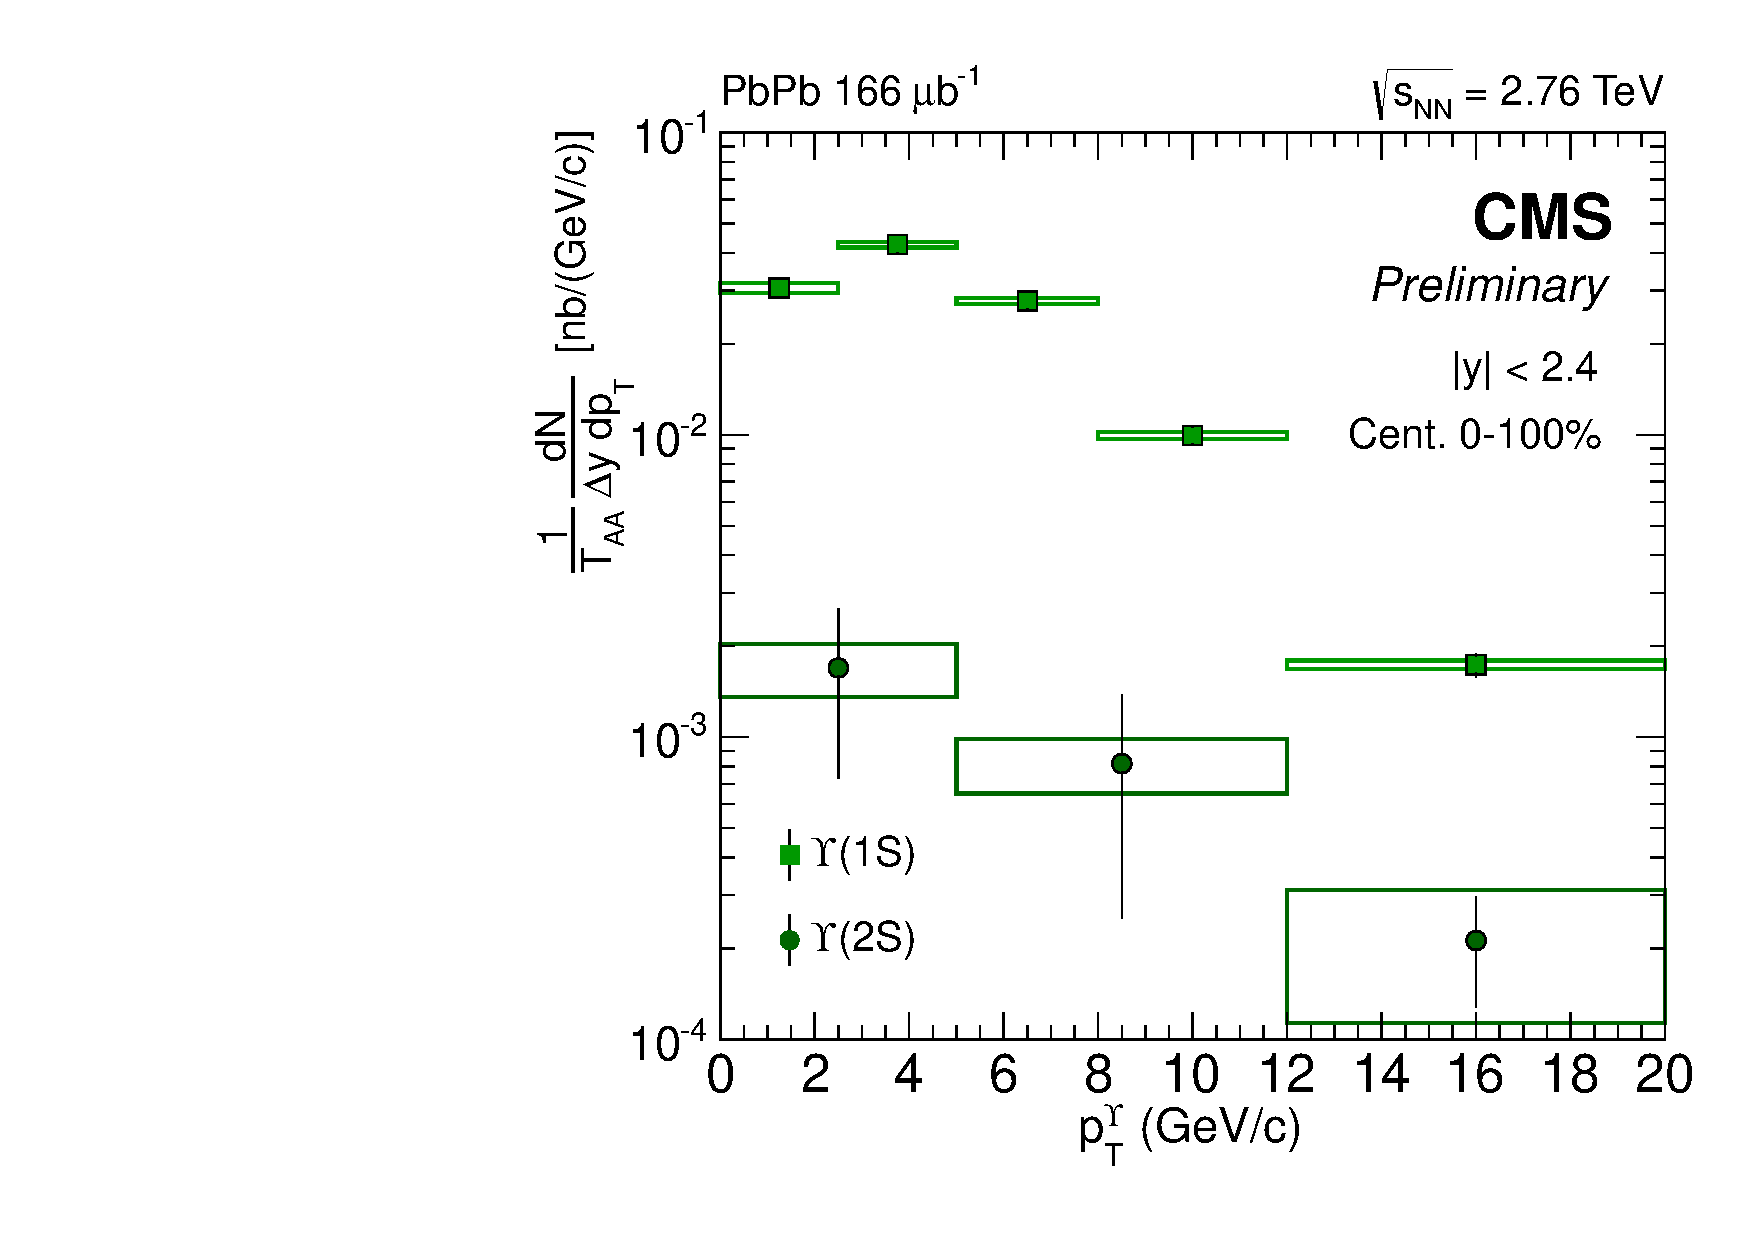
\includegraphics[width=0.65\textwidth]{Chapters/aUpsilon/CS_AAPt.pdf}
    % 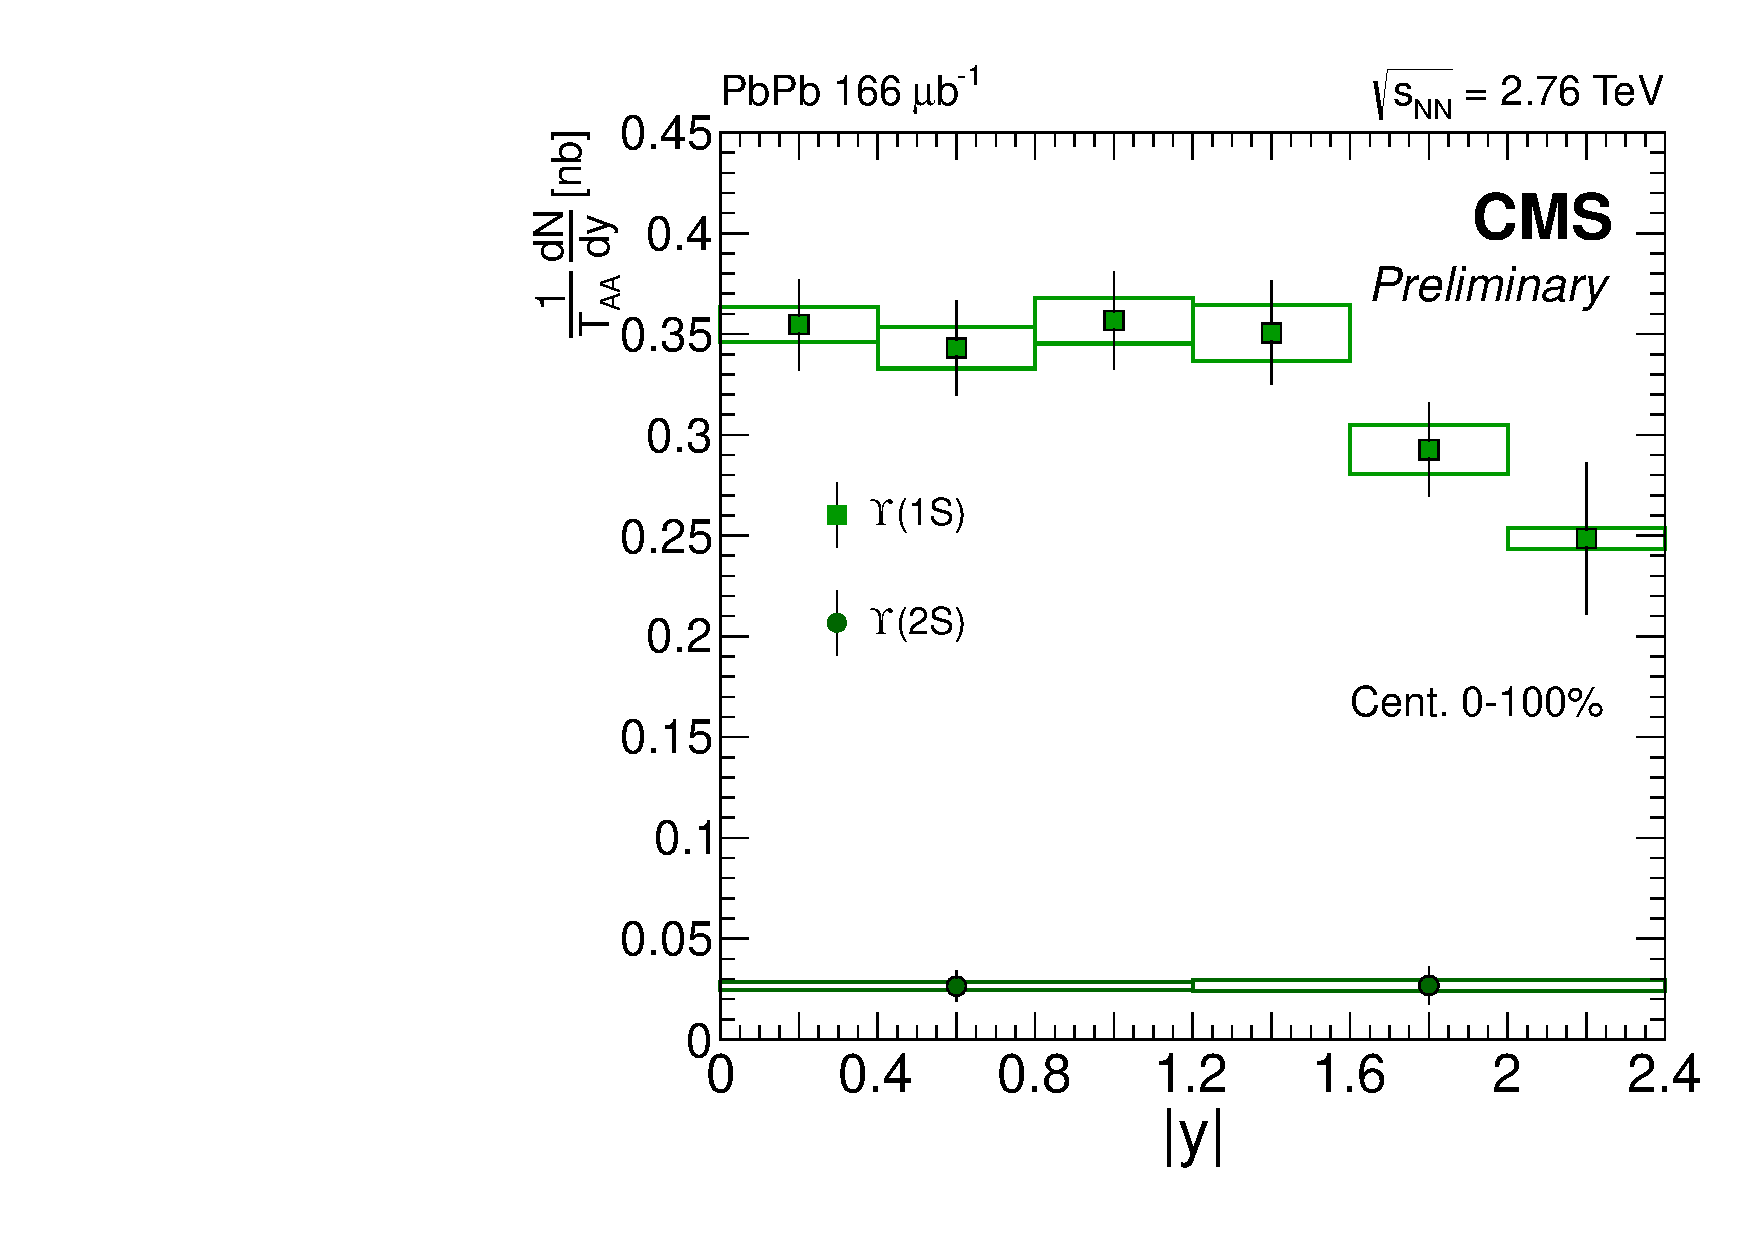
\includegraphics[width=0.7\textwidth]{Chapters/aUpsilon/CS_AA_Rap_lin.pdf}
    \caption{Normalised cross sections for PbPb $\to \PgU(nS) \to \mu\mu$ in $\vert\y\vert < 2.4$, as a function of the \PgU\ transverse momentum. A global luminosity uncertainty (luminosity, tracking efficiency) of 10\% is not displayed.}
    \label{fig:PbPbCrossSections_pt}
  \end{centering}  
\end{figure}

\begin{figure}[h]
  \begin{centering}  
    % 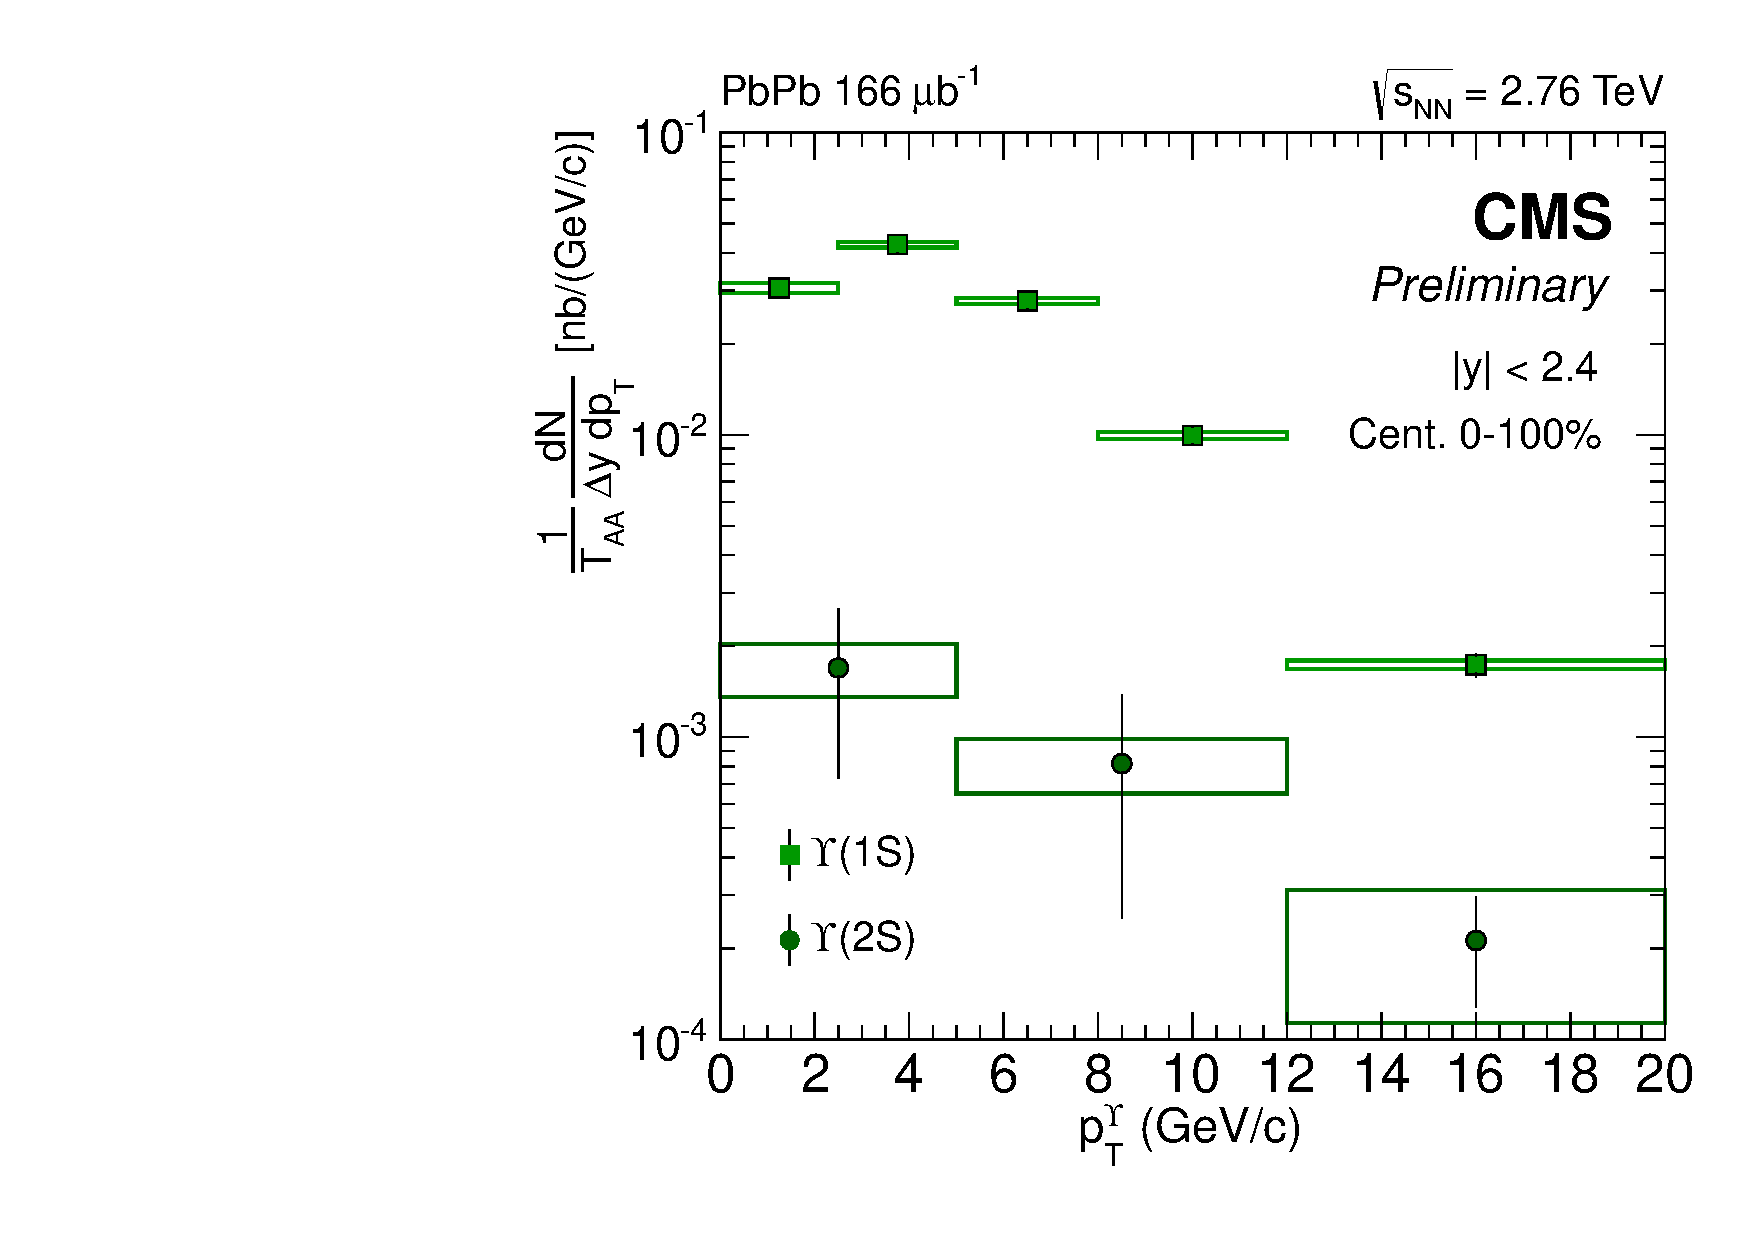
\includegraphics[width=0.7\textwidth]{Chapters/aUpsilon/CS_AAPt.pdf}
    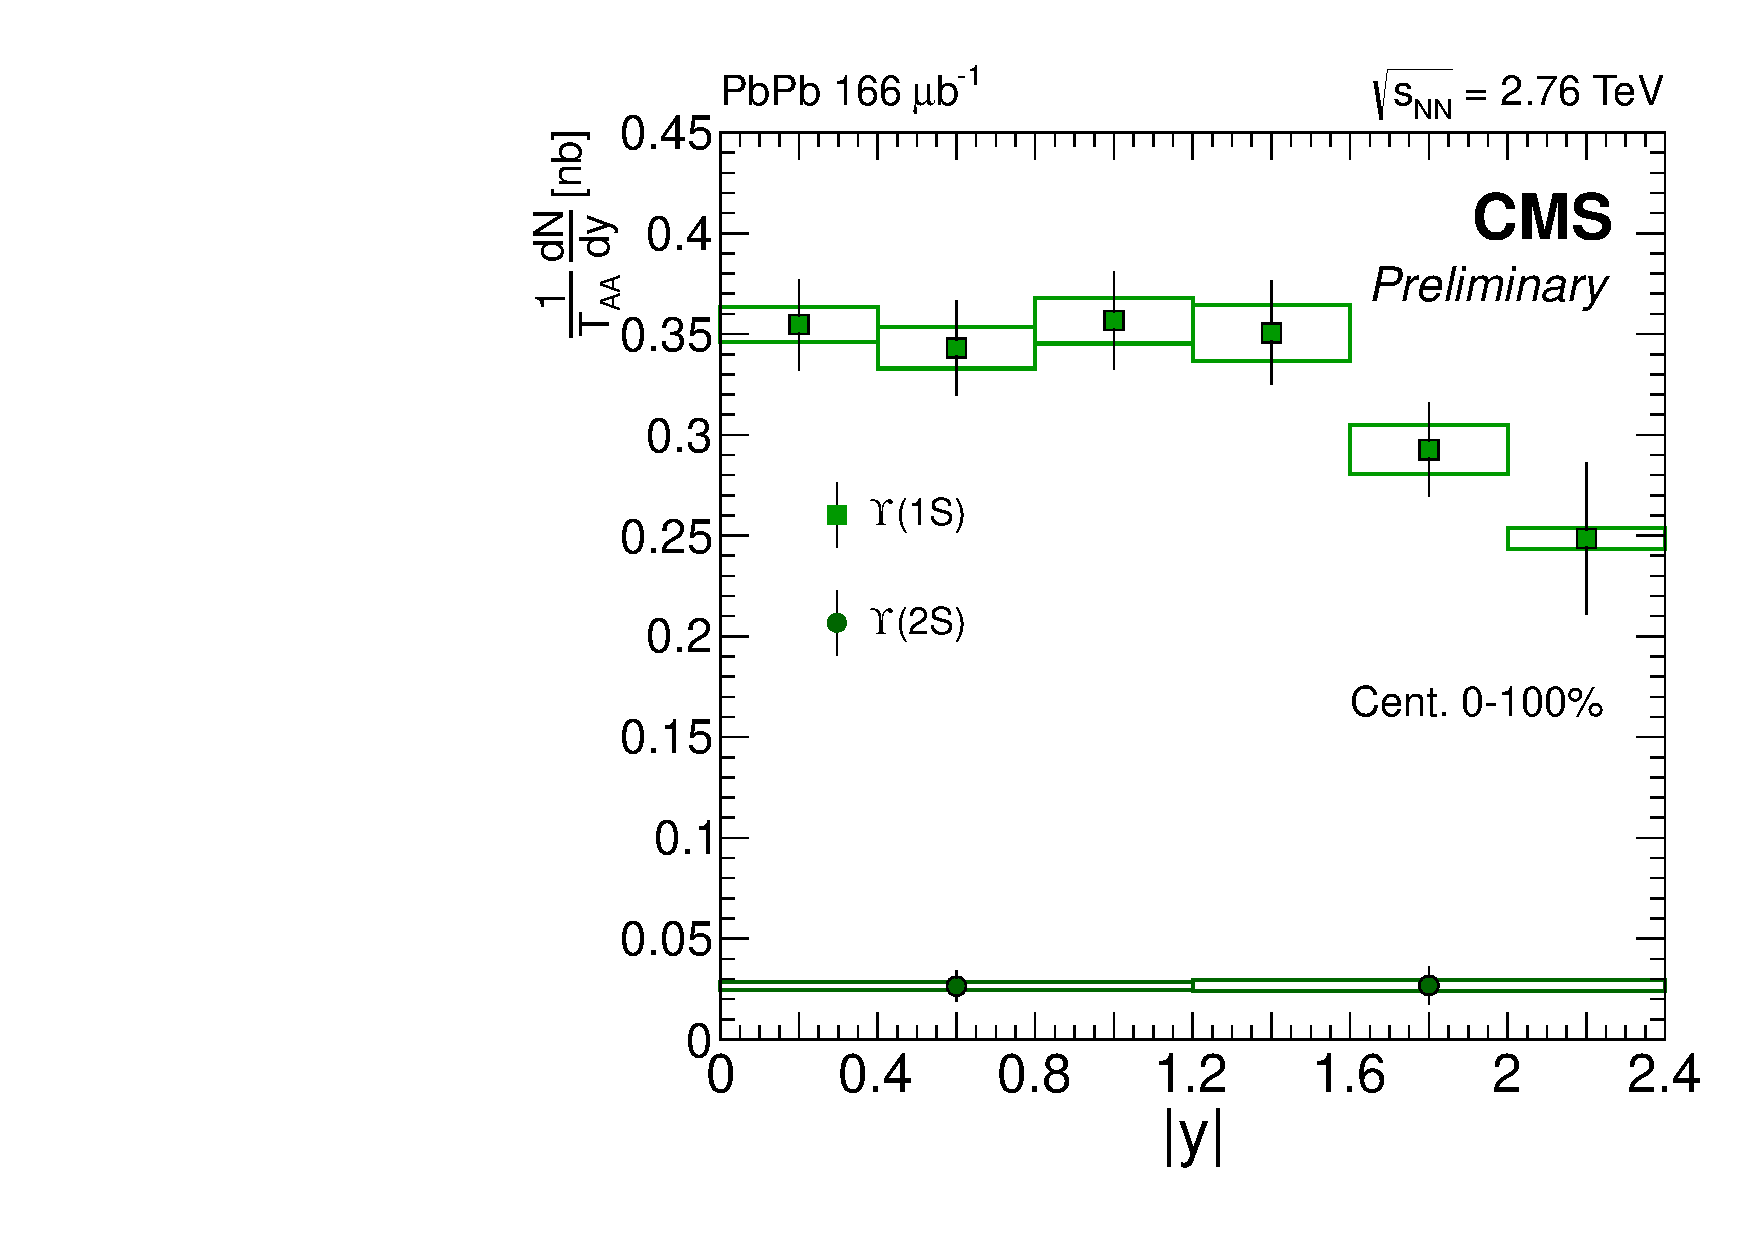
\includegraphics[width=0.65\textwidth]{Chapters/aUpsilon/CS_AA_Rap_lin.pdf}
    \caption{Normalised cross sections for PbPb $\to \PgU(nS) \to \mu\mu$ in $\vert\y\vert < 2.4$, as a function of the \PgU\ rapidity. A global luminosity uncertainty (luminosity, tracking efficiency) of 10\% is not displayed.}
    \label{fig:PbPbCrossSections_y}
  \end{centering}  
\end{figure}

These results represent a first differential measurement of the \PgUb\ spectrum
in tranvserse momentum and rapidity, as well as a significantly
improved measurement of the \PgUa\ up to \pt = 20 \GeVc.


From the computation of \TAA-scaled yields, the comparison with $pp$
results becomes automatic. At first sight, the spectra look
qualitatively similar, with a different normalisation. Additionally, the \PgUb\ looks much less
significant than its $pp$ counterpart: this is the sign of the
known strong suppression of excited states, first measured
in~\cite{HIN-11-007}. To get a quantitative account of the suppression
observed in this measurement, I will now turn to the nuclear
modification factor, \RAA, and present the results for all three \PgU\ states.

Tabulated versions of the invariant yields
will be reported in the next Section~\ref{subsec:raa}, side by side with the tabulated
\RAA\ results.

\subsection{Nuclear modification factor}
\label{subsec:raa}
To compare the production rate of a given particle (hard or soft
probe) in $pp$ to its heavy ion counterpart, one usually invokes the
nuclear modification factor, defined as:

\begin{equation}
  \RAA = \frac{\mathcal{L}_{pp}}{\TAA\NMB} \cdot
  \frac{\textrm{N}(\PgU(nS))_{\textrm{PbPb}}}{\textrm{N}(\PgU(nS))_{pp}} \cdot
  \frac{\eff_{pp, w}}{\eff_{\textrm{PbPb}, w}} 
  \label{eq:raa2}
\end{equation}  

With this definition, \RAA\ is dependent on:
\begin{itemize}
\item[-] the bin in which the raw yields and efficiency corrections
  are considered,
\item[-] \NMB, the total number of minimum bias hadronic events
  recorded in the experiment,
\item[-] $\mathcal{L}_{pp}$, the integrated luminosity recorded in
  $pp$,
\item[-] \TAA, the nuclear overlap function in a given centrality bin, that has the same
  dimension as the luminosity, and accounts for the amount of
  nucleon-nucleon interactions during the time of
  the nucleus-nucleus interaction.
\end{itemize}

Both $pp$ and PbPb quantities have to be recorded at the same
nucleon-nucleon centre-of-mass energy. The centrality dependent results
are usually plotted as a function of \Npart, the number of participating (or wounded)
nucleons in the collision. 
The nuclear modification factor of \PgUa, \PgUb, is measured in bins
of \pt, \y, and \Npart\ in
Figures~\ref{fig:raapt},~\ref{fig:raarap},~\ref{fig:RAAnpart}
respectively.

The PbPb corrected yields and \RAA\ for \PgUa\ and \PgUb\ are tabulated as a function of \pt and \y in Tables~\ref{tab:CSaapttab} and \ref{tab:CSaaraptab}, respectively.

\begin{figure}[h]
  \begin{centering}  
    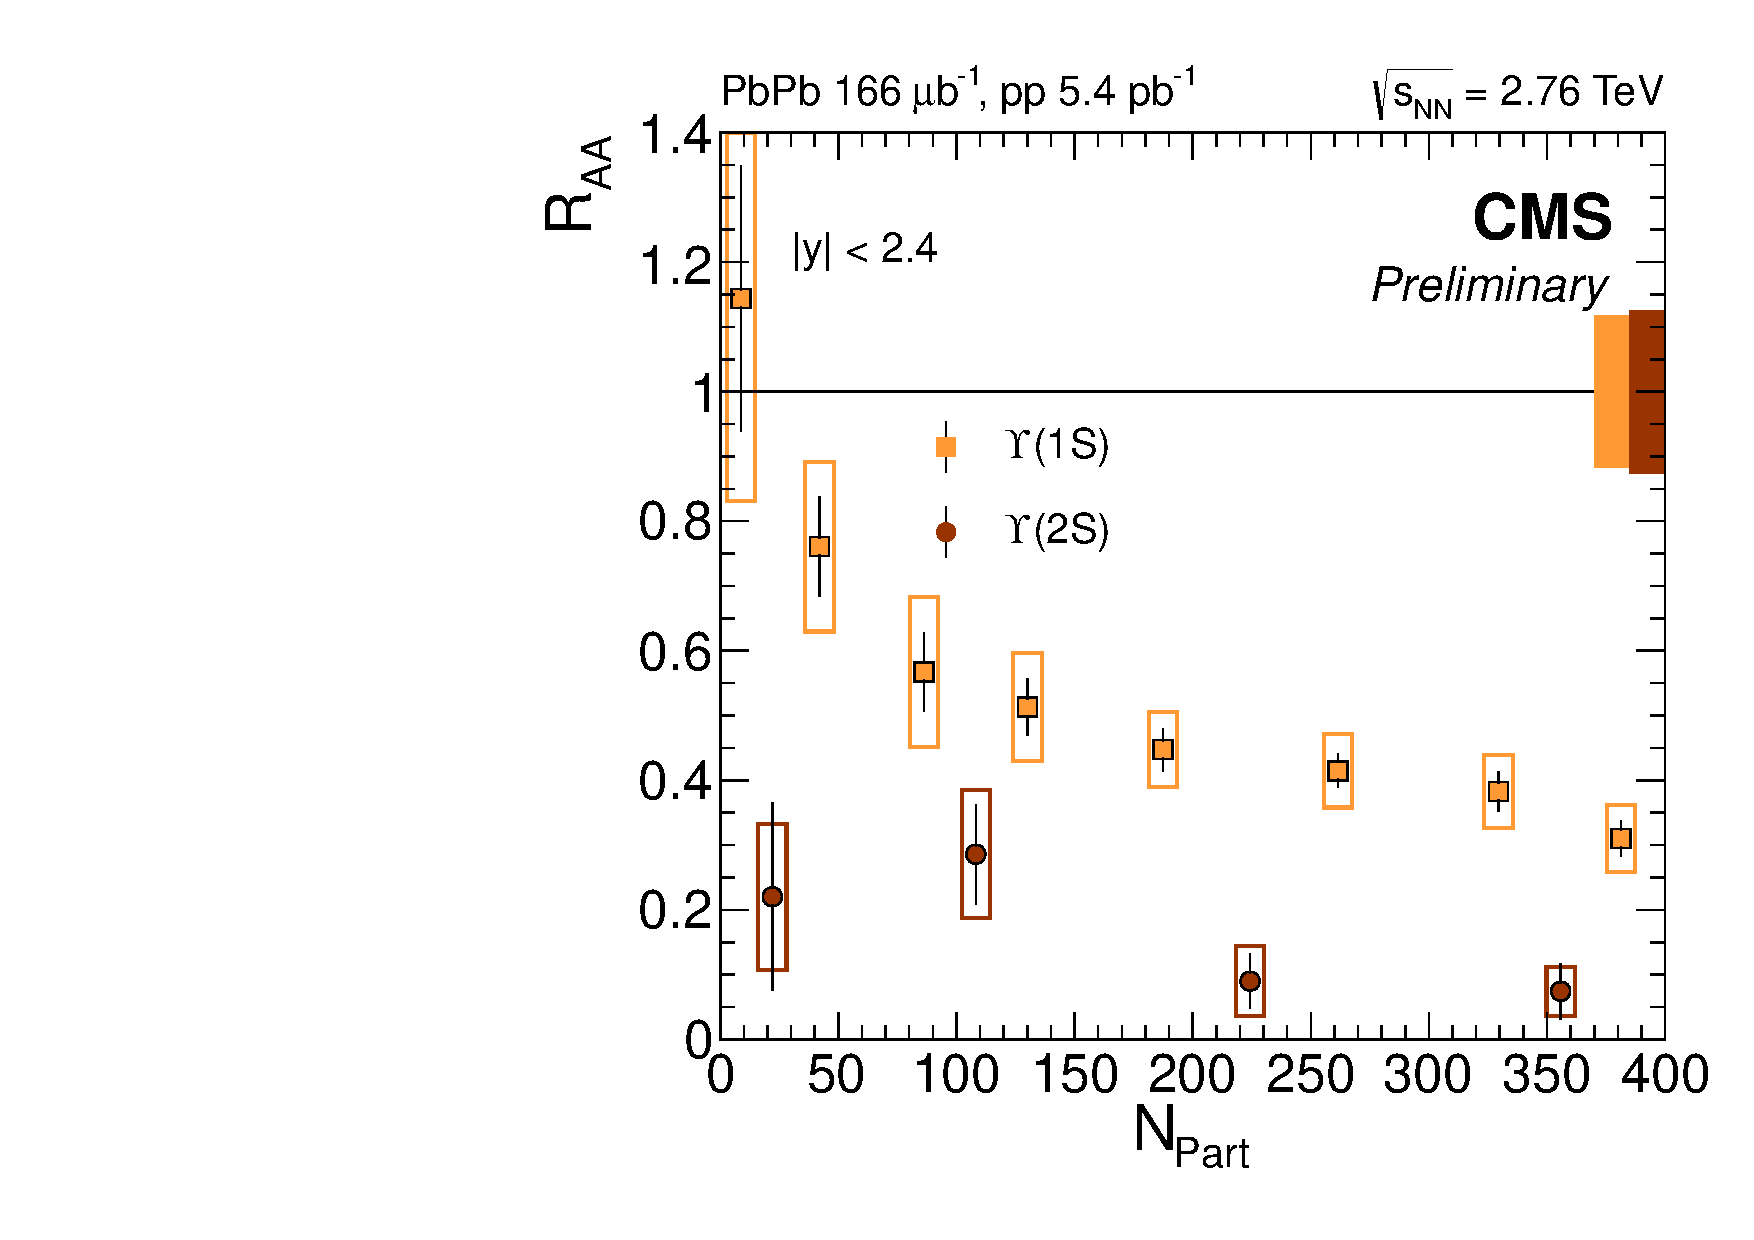
\includegraphics[width=0.7\textwidth]{Chapters/aUpsilon/RAA_nPart_4bins-1.pdf}
    \caption{PbPb nuclear modification factor \RAA\ in PbPb collisions
      at \snn\ = 2.76 \TeV, as a function of the number of participants.}
    \label{fig:RAAnpart}
  \end{centering}  
\end{figure}

The centrality dependence of the suppression has been computed
in various \Npart\ bins for \PgUa\ and \PgUb. Some additional
features should be noted with respect to the previous analysis from
CMS, using a lower $pp$ reference~\cite{11-011}:
\begin{itemize}
\item[-]{the \PgUa\ analysis is now performed with the yield extraction
    method using the `loose' single muon $\pt$ cuts, cf. Section~\ref{sec:sigext_fits},} % $\pt^{\mu_1} > 3.5
    % \GeVc$, $\pt^{\mu_2} > 4 \GeVc$ previously defined in Section
    % \ref{sec:sigext_fits};}
\item[-]{an additional peripheral bin in the 1S result is measured: The
    peripheral 50$-$100\% bin is now splitted into 50$-$70\% and
    70$-$100\%. This is possible thanks to the extended reference as well
    as the improved heavy ion reconstruction,}
\item[-]{to get a clearer impression of the \PgUb\ suppression with
  increasing centrality, a coarser binning than in~\cite{11-011} was
  used: instead of seven bins, one can now find four
  centrality bins, each of them merging two of the bins used in the present Y(1S) analysis.}
\end{itemize}

The choice of having less bins for the \PgUb\ is motivated by the low
significance of this signal overall, yielding only $\sim 200$ \PgUb\
events in PbPb. Furthermore, the previous
analysis of \PgUb\ used as many bins in \PgUb\ and \PgUa\ mostly
because of the yield extraction technique used at the time, taking
the yield ratio $\PgUa / \PgUb$ as the parameter of interest. Now
that the yields are analysed separately for each state, the analysis
does not rely on this ratio parameter anymore.


% \item{The  $pp$ sample used herein results of a much longer data taking
%   period than previously, reducing significantly the uncertainty on the
%   suppression. The Y analysis in pPb (Ref. here: HIN-13-003) has
%   estimated the normalisation ratio between 2011 and 2013  $pp$ cross
%   sections to be (1.6 $\pm$ 0.4), resulting in a difference not greater
%   than 1.5 standard deviations.}
% \end{itemize}

% Table \ref{tab:centraa} reports the invariant yield divided by
% \TAA\ in centrality classes for 1S and 2S in upper and lower
% panels, respectively. Figure \ref{fig:raacompcent} shows the
% corresponding \RAA\ measured in this analysis (1S in orange, 2S in
% blue) compared with the previous measurement (1S in green, 2S in white
% circles.)




\begin{table}[hbtp]
  \begin{centering}
    \begin{tabular}{|c|c|c|}
      \hline
      % Centrality percentiles & 1/\TAA.invariant yield & \RAA\ \\                                               
      Centrality percentiles & $\YPbPb[\PgUa]/\TAA$ [nb] &  \RAA[\PgUa]\ \\                                               
      \hline
      % \pt^{\mu} <$ 3.5 or 4 GeV &  $\frac{dN_{1S}}{\TAA\cdot
      % dy}\cdot B_{\mu\mu}$
      % [nb] & \RAA[\PgUa] \\
      % \hline 
      0-5    &1.12 $\pm$ 0.099 $\pm$ 0.043  &  0.310 $\pm$ 0.027 $\pm$ 0.050  \\  
      5-10   &1.38 $\pm$ 0.112 $\pm$ 0.048  &  0.383 $\pm$ 0.031 $\pm$ 0.055  \\  
      10-20  &1.50 $\pm$ 0.094 $\pm$ 0.048  &  0.415 $\pm$ 0.026 $\pm$ 0.055  \\  
      20-30  &1.62 $\pm$ 0.120 $\pm$ 0.050  &  0.447 $\pm$ 0.033 $\pm$ 0.057   \\  
      30-40  &1.85 $\pm$ 0.161 $\pm$ 0.075  &  0.513 $\pm$ 0.044 $\pm$ 0.082   \\  
      40-50  &2.05 $\pm$ 0.222 $\pm$ 0.106  &  0.567 $\pm$ 0.061 $\pm$ 0.115   \\  
      50-70  &2.76 $\pm$ 0.281 $\pm$ 0.120  &  0.764 $\pm$ 0.077 $\pm$ 0.130    \\  
      70-100 &4.15 $\pm$ 0.746 $\pm$ 0.292  & 1.150 $\pm$ 0.207 $\pm$ 0.314      \\  % 
      \textbf{0-100}  &\textbf{1.537 $\pm$ 0.081 $\pm$ 0.028}   & \textbf{0.425 $\pm$ 0.029$\pm$ 0.070} \\   
      \hline 
       $pp$     &3.544 $\pm$ 0.067 $\pm$ 0.109 & --- \\
      \hline  
      \hline          
      % \pt^{\mu} <$ 4 GeV &  $\frac{d\sigma_{2S}}{\TAA\cdot dy}\cdot B_{\mu\mu}$
      % [nb] & \RAA[\PgUb]   \\
      % \pt^{\mu} <$ 4 GeV 
      &  $\YPbPb[\PgUb]/\TAA$ [nb] 
      % $\frac{d\sigma_{2S}}{\TAA\cdot dy}\cdot B_{\mu\mu}$
      % [nb] 
      & \RAA[\PgUb]   \\
      \hline
      0-10   & 0.076 $\pm$ 0.045 $\pm$0.039  & 0.074 $\pm$ 0.044 $\pm$ 0.038 \\  
      10-30  & 0.092 $\pm$ 0.044 $\pm$0.056  & 0.090 $\pm$ 0.042 $\pm$ 0.054  \\  
      30-50  & 0.293 $\pm$ 0.079 $\pm$0.103  & 0.286 $\pm$ 0.077 $\pm$ 0.100   \\  
      50-100 & 0.226 $\pm$ 0.149 $\pm$0.116  & 0.220 $\pm$ 0.145 $\pm$ 0.113   \\  
      \textbf{0-100}  & \textbf{0.119 $\pm$ 0.029 $\pm$ 0.002} & \textbf{0.116 $\pm$ 0.028  $\pm$ 0.022}  \\  
      \hline 
       $pp$     & 1.026 $\pm$ 0.042 $\pm$  0.037  & --- \\
      \hline 
    \end{tabular}
    \caption{\TAA-scaled cross sections and nuclear modification
      factors \RAA\ for different centrality bins (and for
      centrality-integrated value, bold font) for \PgUa\ and \PgUb in
      PbPb collisions at \snn\ = 2.76 TeV.}
    \label{tab:centraa}
  \end{centering}
\end{table}

\begin{figure}[h]
  \begin{centering}  
    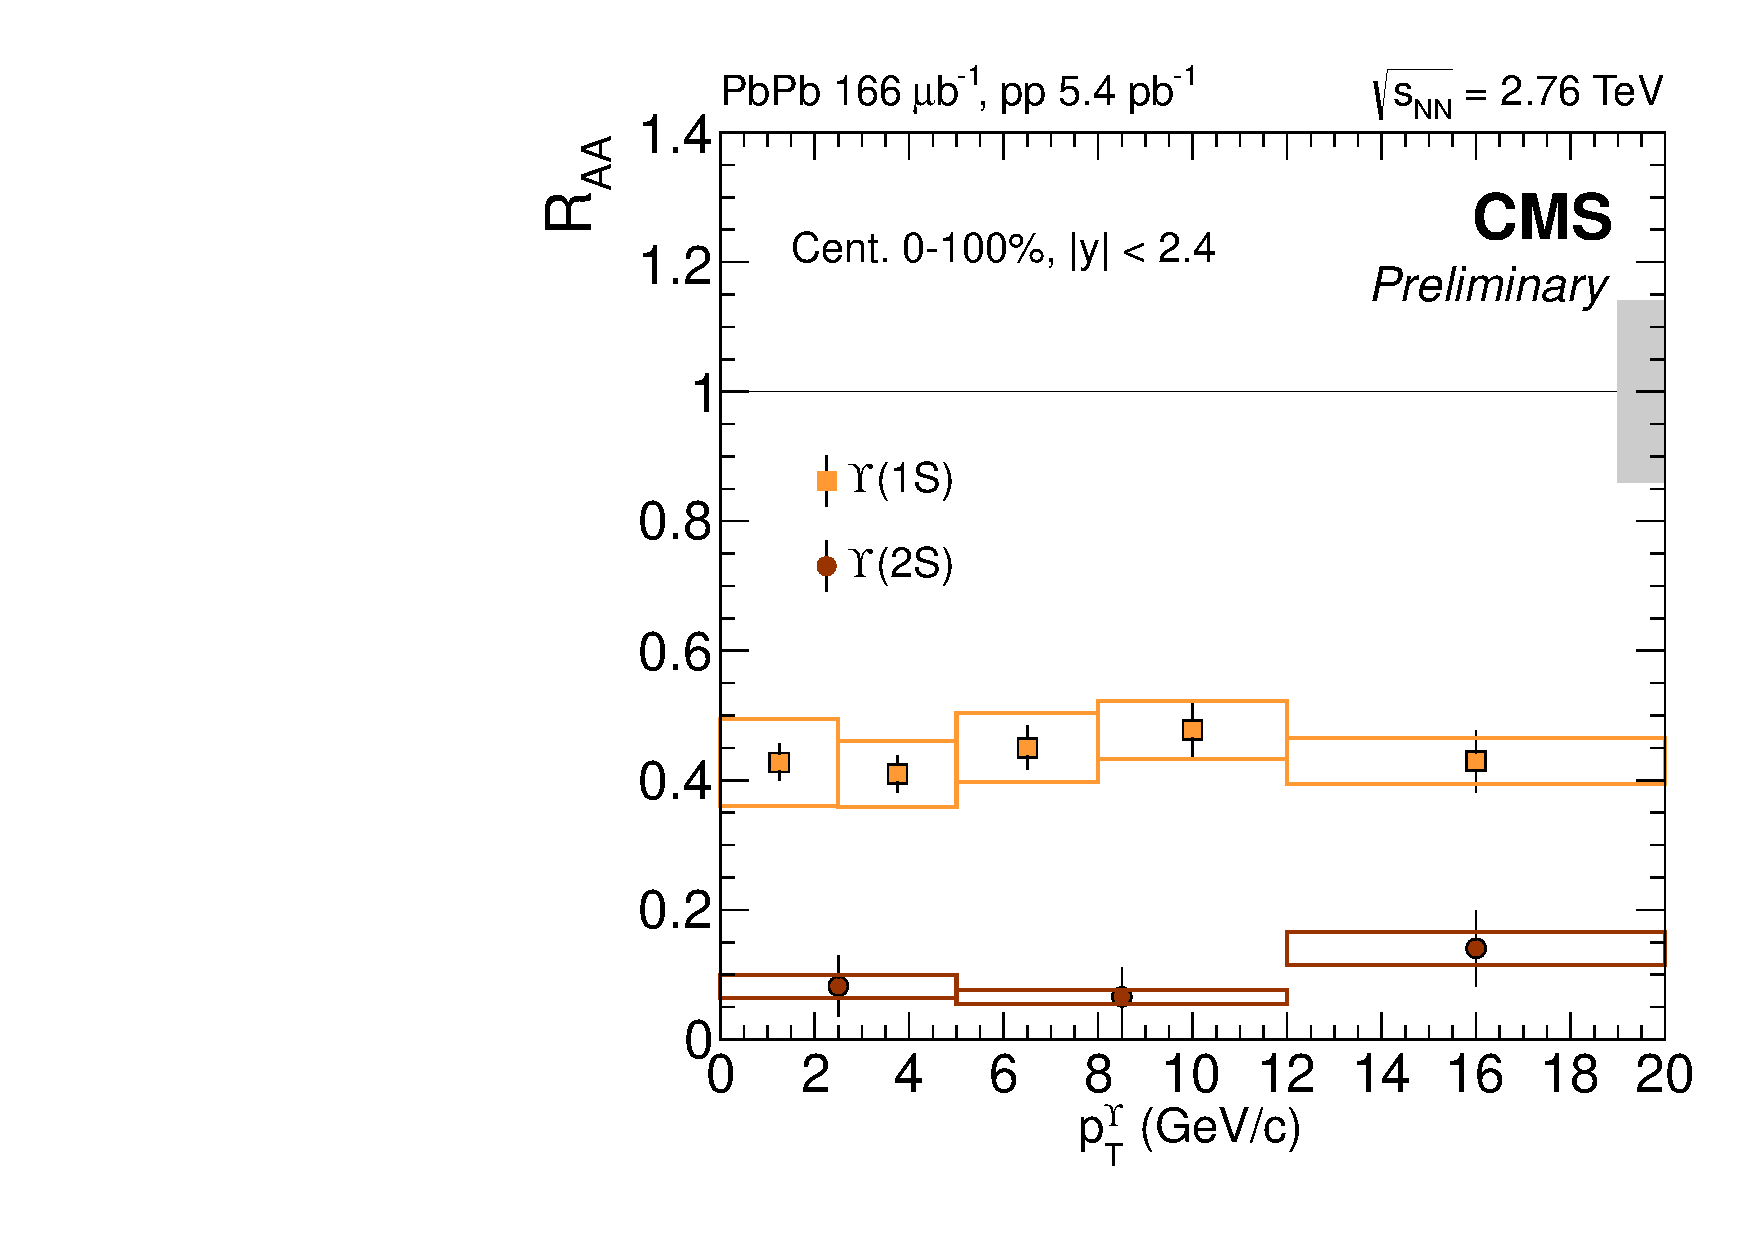
\includegraphics[width=0.65\textwidth]{Chapters/aUpsilon/RAA_Pt-1.pdf}
    \caption{PbPb nuclear modification factor of \PgUa\ and \PgUb\ in PbPb collisions
      at \snn\ = 2.76~\TeV, as a function of the \PgU\ transverse momentum. The gray error bar at unity is the global
      systematic uncertainty due to $pp$ tracking efficiency and luminosity.}
    \label{fig:raapt}
  \end{centering}  
\end{figure}

\begin{figure}[h]
  \begin{centering}  
    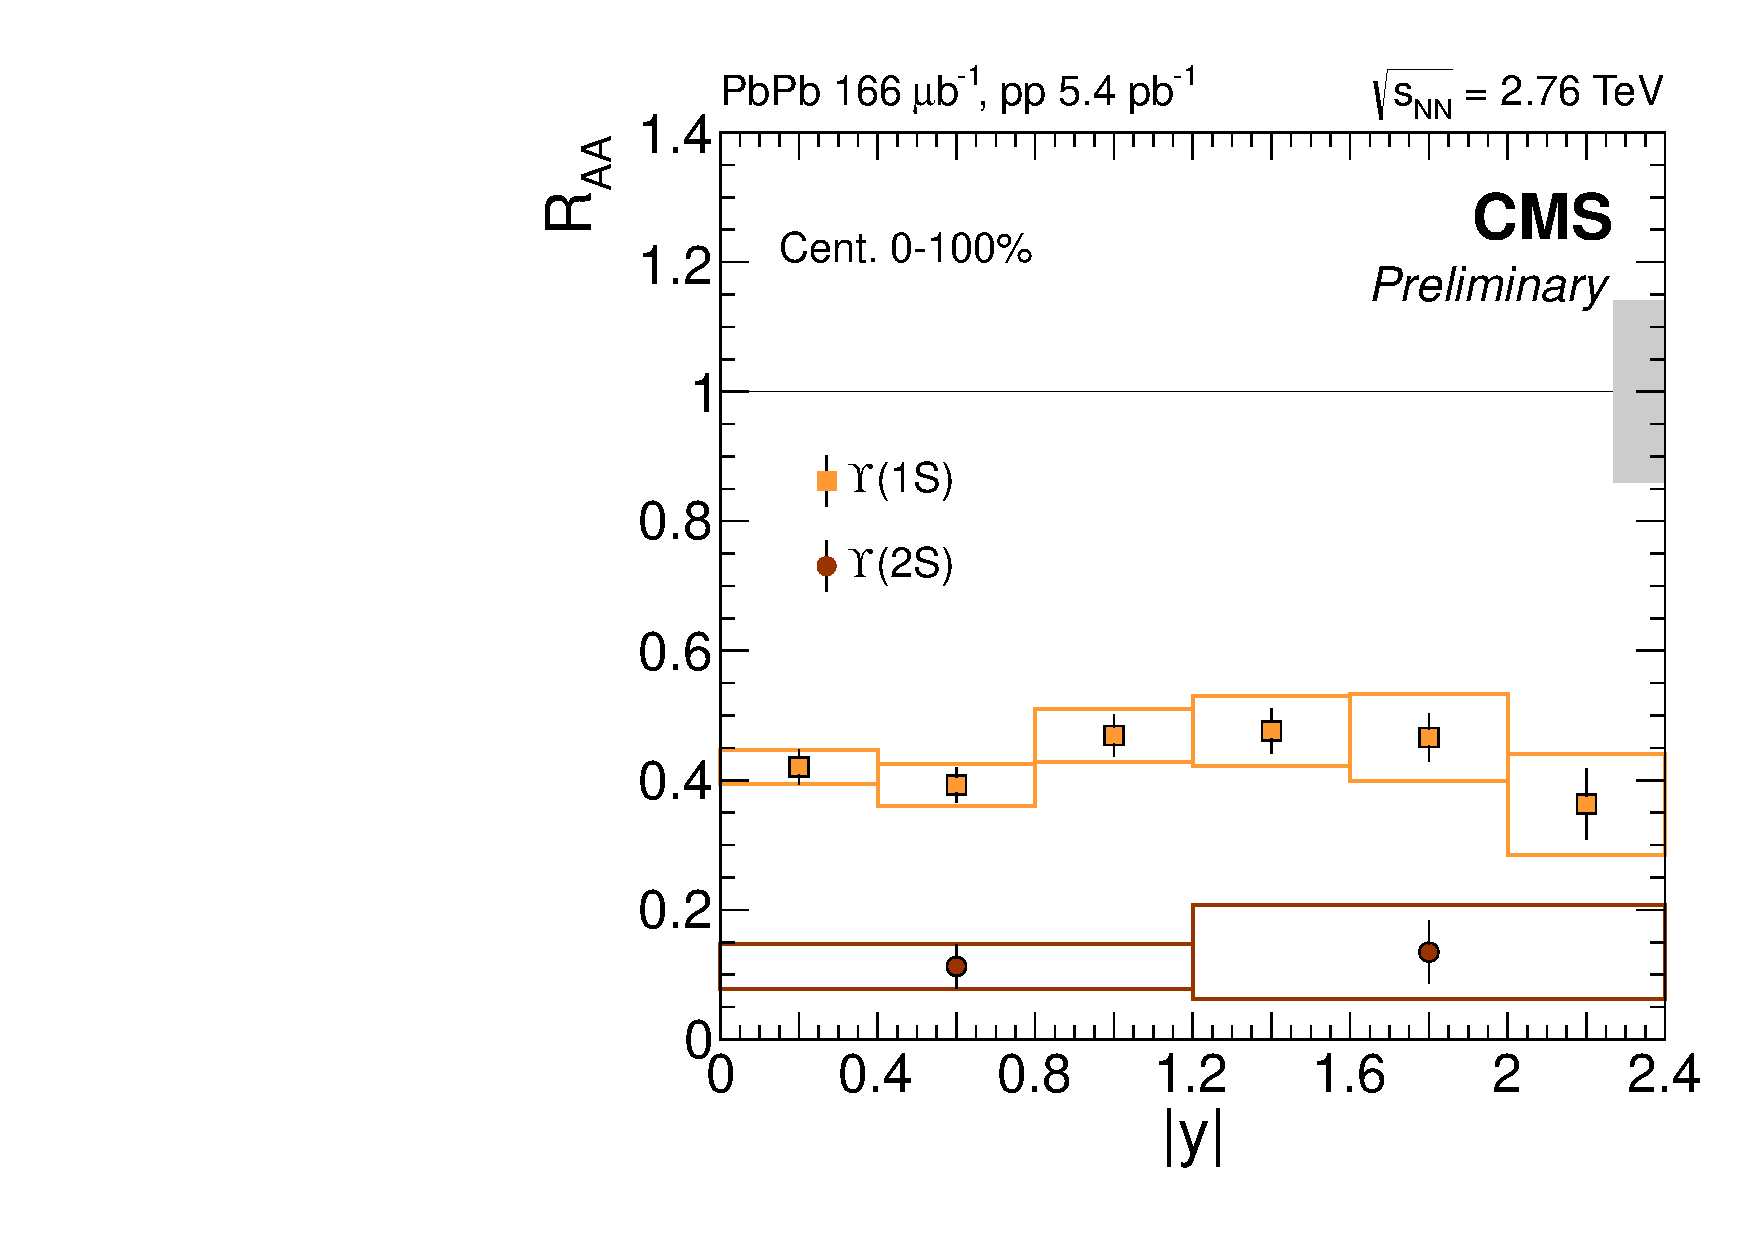
\includegraphics[width=0.65\textwidth]{Chapters/aUpsilon/RAA_Rap-1.pdf}
    \caption{PbPb nuclear modification factor of \PgUa\ and \PgUb\ in PbPb collisions
      at \snn\ = 2.76 \TeV, as a function of the \PgU\ rapidity. The gray error bar at unity is the global
      systematic uncertainty due to $pp$ tracking efficiency and luminosity.}
    \label{fig:raarap}
  \end{centering}  
\end{figure}

\begin{table}[hbtp]
  \begin{centering}
    \begin{tabular}{|c|c|c|}                                      
      \hline
      % $|y| < $2.4 & $\frac{d\sigma_{1S}}{dyd\pt}\cdot B_{\mu\mu}$[nb
      % c/GeV] & \RAA[\PgUa] \vline \\
      $|y| < $2.4 & $\YPbPb[\PgUa]/\TAA$ [nb] & \RAA[\PgUa]  \\
      \hline
      \pt [\GeVc] $<$ 2.5       & 0.0306 $\pm$ 0.0017 $\pm$ 0.0011  & 0.428 $\pm$ 0.029 $\pm$ 0.067  \\
      2.5 $<$ \pt [\GeVc] $<$ 5 & 0.0426 $\pm$ 0.0026 $\pm$ 0.0008  & 0.410 $\pm$ 0.029 $\pm$ 0.051\\
      5 $<$ \pt [\GeVc] $<$ 8   & 0.0277 $\pm$ 0.0018 $\pm$ 0.0007  & 0.450 $\pm$ 0.034 $\pm$ 0.053\\
      8 $<$ \pt [\GeVc] $<$ 12  & 0.00994 $\pm$ 0.00074 $\pm$ 0.0002& 0.478 $\pm$ 0.042 $\pm$ 0.044  \\
      12 $<$ \pt [\GeVc] $<$ 20 & 0.00174 $\pm$ 0.00016 $\pm$ 5.4$\cdot 10^{-5}$ & 0.430 $\pm$ 0.048 $\pm$ 0.035\\

      \hline
      $|y| < $2.4 & $\dfrac{1}{\TAA} \cdot \dfrac{1}{\Delta y} \cdot \dfrac{\text{d}N\left( AA\rightarrow
          \PgU(nS)X\right)}{\text{d}\pt} \cdot B_{\mu\mu}$ [nb] & \RAA[\PgUb]  \\
      \hline
      \pt [\GeVc] $<$ 5          & 0.00169 $\pm$ 0.00096 $\pm$0.00033 & 0.082$\pm$ 0.047 $\pm$ 0.018 \\%  0.0821$\pm$ 0.0471 $\pm$ 0.0182 \\  
      5 $<$ \pt [\GeVc] $<$ 12   & 0.00082 $\pm$ 0.00056 $\pm$0.00016 & 0.066$\pm$ 0.046 $\pm$ 0.011 \\%  0.0656$\pm$ 0.0457 $\pm$ 0.0115 \\  
      12 $<$ \pt [\GeVc] $<$ 20  & 0.00021 $\pm$ 8.5$\cdot 10^{-5}$ $\pm$~9.9$\cdot 10^{-5}$ & 0.141$\pm$ 0.058 $\pm$ 0.025 \\  
      \hline
    \end{tabular}
    \caption{Normalized yields $\YPbPb/\TAA$ and \RAA\ as a function
      of $\pt$ for \PgUa\ (top) and \PgUb\ (bottom) states, in
      PbPb collisions at \snn\ = 2.76 TeV. Listed
      uncertainties are statistical (first) and systematic (second).}  
    \label{tab:CSaapttab}
  \end{centering}
\end{table}

\begin{table}[hbtp]
\begin{centering}
\begin{tabular}{|c|c|c|c|}                                      
\hline
%p$^{\mu\mu}_{T} > $0 GeV/c & $\frac{d\sigma_{1S}}{dy}\cdot B_{\mu\mu}$
%[nb] & \RAA[\PgUa]  \vline \\
%p$^{\mu\mu}_{T} > $0 GeV/c 
& $\YPbPb[\PgUa]/\TAA$ [nb] & \RAA[\PgUa]  \\
\hline
$|y| <$ 0.4        & 0.355$\pm$ 0.022$\pm$  0.007 & 0.421$\pm$0.027$\pm$ 0.027\\  
0.4 $< |y| <$ 0.8  & 0.343$\pm$ 0.023$\pm$  0.012 & 0.393$\pm$0.027$\pm$ 0.033 \\  
0.8 $< |y| <$ 1.2  & 0.357$\pm$ 0.024$\pm$  0.019 & 0.469$\pm$0.032$\pm$ 0.041\\  
1.2 $< |y| <$ 1.6  & 0.352$\pm$ 0.025$\pm$  0.013 & 0.476$\pm$0.035$\pm$ 0.054\\  
1.6 $< |y| <$ 2    & 0.300$\pm$ 0.025$\pm$  0.019 & 0.466$\pm$0.037$\pm$ 0.067\\  
2 $< |y| <$ 2.4    & 0.249$\pm$ 0.037$\pm$  0.007 & 0.363$\pm$0.055$\pm$ 0.078 \\  
\hline   


\hline
%p$^{\mu\mu}_{T} < $0 GeV/c & $\frac{d\sigma_{2S}}{dy}\cdot B_{\mu\mu}$
%[nb] & \RAA[\PgUb] \vline \\
%p$^{\mu\mu}_{T} < $0 GeV/c 
& $\YPbPb[\PgUb]/\TAA$ [nb] & \RAA[\PgUb]  \\
\hline
$|y| <$ 1.2       & 0.0264 $\pm$0.0077 $\pm$ 0.0019 & 0.113 $\pm$ 0.034 $\pm$ 0.034 \\  
1.2 $< |y| <$ 2.4 & 0.0268 $\pm$0.0095$\pm$  0.0025 & 0.135 $\pm$ 0.049 $\pm$ 0.073  \\  
\hline

\end{tabular}
\caption{Normalized yields $\YPbPb/\TAA$ and \RAA\ as a function of
  $y$ for \PgUa (top) and \PgUb\ (bottom) states in PbPb collisions at
  \snn\ = 2.76 TeV. Listed
uncertainties are statistical (first) and systematic (second).} 
\label{tab:CSaaraptab} 
\end{centering}
\end{table}

% \subsection{double-differential ?}
\subsection{Systematic uncertainties on \texorpdfstring{\RAA}{RAA}}
A break-down of the systematic uncertainties is given in the following
Table \ref{tab:breakdown} for the \pt- and \y-dependent analyses of
\PgUa. The listed uncertainties from left to right
are:
\begin{itemize}
\item[-] statistical uncertainty from the nominal fit to the
  $pp$ yield,
\item[-] systematic uncertainty from fit variations on $pp$ data,
\item[-] systematic uncertainty from fit variations on PbPb data,
\item[-] generator level shape variation uncertainties on $pp$ and PbPb corrections \acc\eff$_{w}$,
\item[-] Tag and Probe uncertainty for efficiency corrections in
  $pp$ data,
\item[-] Tag and Probe uncertainty for efficiency corrections in PbPb data,
\item[-] \textbf{correlated sub-total}: total of \textit{correlated} systematic uncertainties, computed as the quadratic sum of the previous items,
\item[-] \textbf{total}: quadratic sum of correlated and `global' uncertainties (common to all points, i.e. luminosities
  and tracking efficiencies).
\end{itemize}
\begin{sidewaystable}[h]
    \begin{centering}
      {\large
        \begin{tabular}{|c|c|c|c|c|c|c|c|c|}
          \hline
          $\pt$ bin & Stat. (pp) & Stat. (AA) & Syst(PDF)$_{pp}$ & Syst(PDF)$_{AA}$ & TNP$_{pp}$ &  TNP$_{AA}$ & Correlated &
          total\\
          \hline
          \pt [\GeVc] $<$ 2.5       & 0.034 & 0.057 & 0.076 & 0.091 & 0.007 & 0.040 & 0.133 & 0.151\\
          2.5 $<$ \pt [\GeVc] $<$ 5 & 0.032 & 0.061 & 0.050 & 0.065 & 0.006 & 0.040 & 0.103 & 0.126\\
          5 $<$ \pt [\GeVc] $<$ 8   & 0.034 & 0.066 & 0.039 & 0.125 & 0.006 & 0.038 & 0.146 & 0.163  \\
          8 $<$ \pt [\GeVc] $<$ 12  & 0.046 & 0.074 & 0.023 & 0.043 & 0.006 & 0.035 & 0.081 & 0.108 \\
          12 $<$ \pt [\GeVc] $<$ 20 & 0.060 & 0.093 & 0.008 & 0.038 & 0.007 & 0.034 & 0.071 & 0.101\\
          \hline
          \hline
          $|y| <$ 0.4        & 0.035 & 0.064 &  0.030 & 0.055 & 0.004 & 0.010 & 0.063 & 0.005 \\
          0.4 $< |y| <$ 0.8  & 0.035 & 0.068 &  0.026 & 0.110 & 0.004 & 0.011 & 0.114 & 0.009\\
          0.8 $< |y| <$ 1.2  & 0.039 & 0.068 &  0.038 & 0.175 & 0.004 & 0.018 & 0.180 & 0.019 \\
          1.2 $< |y| <$ 1.6  & 0.042 & 0.074 &  0.039 & 0.093 & 0.007 & 0.053 & 0.114 & 0.010 \\
          1.6 $< |y| <$ 2    & 0.052 & 0.085 &  0.051 & 0.216 & 0.012 & 0.108 & 0.247 & 0.038 \\
          2 $< |y| <$ 2.4    & 0.079 & 0.151 &  0.082 & 0.281 & 0.015 & 0.150 & 0.329 & 0.066\\
          \hline
        \end{tabular}
        \caption{Systematic uncertainties recap for \PgUa, in 
          (\pt,\y)-differential \RAA\ analyses. }  
        \label{tab:breakdown}
      }
    \end{centering}
\end{sidewaystable}

Table \ref{tab:breakdownPart} sums up the systematic uncertainties
used in the centrality dependence result.
\begin{itemize}
\item[-] systematic uncertainty from fit variations on PbPb data,
\item[-] efficiency correction, from tag-and-probe in
  $pp$ data,
\item[-] uncertainty on the value of the nuclear thickness function,
\item[-] global $pp$ uncertainty: summing up $\mathcal{L}_{pp}$, integrated
  for $pp$ efficiency, statistical and systematic
  uncertainty from fitting,
\item[-] total of 'correlated' point-to-point
  systematic uncertainties, computed as the quadratic sum of the four
  previous columns,
\item[-] total of 'correlated' and global uncertainty.
\end{itemize}
\begin{table}[hbtp]
  \begin{centering}
    \begin{tabular}{|c|c|c|c|c|c|c|}
      \hline
      1S Centrality & Syst(PDF)$_{AA}$ & TNP$_{AA}$ & T$_{AA}$ &
      Global  $pp$ & Correlated & total\\
      \hline
      0-5   &0.144 &0.036 &0.041 &0.035 &0.160 &0.164 \\
      5-10  &0.120 &0.038 &0.046 &0.035 &0.141 &0.146 \\
      10-20 &0.103 &0.037 &0.052 &0.035 &0.129 &0.134\\
      20-30 &0.085 &0.038 &0.066 &0.035 &0.122 &0.127\\
      30-40 &0.120 &0.038 &0.084 &0.035 &0.157 &0.161\\
      40-50 &0.157 &0.038 &0.109 &0.035 &0.199 &0.202\\
      50-70 &0.054 &0.039 &0.147 &0.035 &0.167 &0.171\\
      70-100&0.215 &0.039 &0.154 &0.035 &0.271 &0.273\\
      \hline
      2S Centrality & Syst(PDF)$_{AA}$ & TNP$_{AA}$ & T$_{AA}$ &
      Global  $pp$ & Correlated & total\\
      \hline
      0-10 &  0.458 &0.035 &0.043 &0.056 &0.510 &0.513 \\
      10-30 & 0.560 &0.036 &0.058 &0.056 &0.603 &0.605 \\
      30-50 & 0.255 &0.036 &0.093 &0.056 &0.346 &0.350 \\
      50-100 &0.440 &0.036 &0.150 &0.056 &0.512 &0.515 \\
      \hline
    \end{tabular}
    \caption{Systematic uncertainties recap for \PgUa\ and $\PgUb$, in
      bins of centrality. }  
    \label{tab:breakdownPart}
  \end{centering}
\end{table} 

% \subsection{Yields from fitting}
%\vfill\newpage
\subsection{Upper limits on \texorpdfstring{\PgUc}{Y(3S)} production in PbPb collisions}
\label{sec:Y3S}

Once the signal is extracted from the maximum likelihood fit,
we employ the Feldman-Cousins (FC) method to set a limit at the $95\%$ confidence level~\cite{PhysRevD.57.3873}.
While the expected limit on the nuclear modification factor is close to a
non-physical (negative) limit, %(i.e. $\RAA(\PgUc) \leq  0$),
the FC prescription guarantees a physically meaningful result and tells us how to smoothly
transition from a one-sided limit to a two-sided interval. In other words, this method will return a two-sided interval
in the case of a significant result, and an upper limit in the case of a non-significant result, the transition
between the two cases being smooth and well-defined from a statistical point of view (i.e. with
a proper coverage).
% % The FC prescription is described in detail in Ref.~\cite{FC}. % Ref missing!
% It uses a likelihood ratio as an ordering principle for selecting the acceptance
% region and creating confidence bands. The likelihood ratio is defined as the following:
% \begin{equation}
%   Q(x)=\frac{P(x|\RAA(\PgUc)_{0})}{P(x|\RAA(\PgUc)_{\text{max}})} \,,
% \end{equation}
% where $Q(x)$ is a likelihood ratio for given $\raa(\PgUc)$, x,  a given $\raa(\PgUc)$ and finally $\raa(\PgUc)_{0}$,
% and $\raa(\PgUc)_{\text{max}}$ is the $\raa(\PgUc)$ for the maximum likelihood among all possible $\raa(\PgUc)$ values.

The Feldman Cousins method is applied via its implementations in
RooStats~\cite{Moneta:2010pm}. In practice the class \verb-HypoTestInverter- is used, with two possible settings: frequentist
(using pseudo-experiments) or asymptotic (using asymptotic formulae). The latter is less reliable and
can only be used as a fast cross-check. The test statistic used is a profile likelihood ratio.

In the lack of MC simulation for the $\PgUc$, we assume the ratio of PbPb to  $pp$ efficiencies to be the same for the $\PgUb$ and $\PgUc$, and
take the value (0.95) from the $\PgUb$ simulation.

Systematic uncertainties are included as nuisance parameters in the fit, with a log-normal distribution. The following systematic uncertainties are included for now:

\begin{itemize}
\item $T_{AA}$ (6.2\%),
\item  $pp$ luminosity (3.7\%),
\item ratio of efficiencies between  $pp$ and PbPb data (including the systematic uncertainty on tag and probe) (5.3\%),
\item number of background events in  $pp$ data (from the fit variations) (4\%),
\item number of background events in PbPb data (from the fit variations) (2\%),
\item number of signal events in  $pp$ data (from the fit variations) (8\%),
\item number of signal events in PbPb data (from the fit variations) (20\%).
\end{itemize}

% This list will be updated soon to match the systematic uncertainties used in the rest of the analysis.

A reliable systematic uncertainty on the $\PgUc$ in PbPb data could not be determined from fit variations, given its non significant yield. For this reason,
this systematic uncertainty was deduced in the following way: 
$\textrm{syst} (\PgUa, \textrm{PbPb}) \times \textrm{syst} (\PgUc, \textrm{pp}) / \textrm{syst} (\PgUa, \textrm{pp})$, which gives $0.11 \times 0.08/0.045 = 0.20$.

Using the asymptotic calculation, we obtain an upper limit $\RAA(\PgUc)<0.13$ at 95\% C.L. Using the full frequentist calculation
(using pseudo-experiments), we obtain

\begin{eqnarray*}
  \RAA(\PgUc) &<& 0.14 \text{   at 95\% C.L.}\\ \nonumber
  \RAA(\PgUc) &<& 0.08 \text{   at 68\% C.L.} \nonumber
\end{eqnarray*}


The result of the scan is shown on Fig.~\ref{fig:3SUL}, on the left for the asymptotic calculation and on the right for the frequentist
calculation. Visually, the upper limit is obtained from the place where the 
observed $CL_s$ (red dots) crosses the horizontal threshold (red line, at $0.05 = 1-0.95$ for 95\% C.L.). Fig.~\ref{fig:3SUL_68} shows the scan for the frequentist
calculation, zoomed in on smaller values of $\RAA(\PgUc)$ for the determination of the 68\% C.L. upper limit.


% The confidence interval calculator is tried as well in
% estimating the 95$\%$ confidence interval of the 2S yield, using the asymptotic approach, as a cross-check. 
% The yield extracted of the 2S confidence region at 95\% C.L. is [60,225], with a
% maximum peaking at about 150 candidates, which is compatible with a direct ML fit. Indeed, the latter gives 
% [101,184] at 68\% C.L., or [62,225] at the 95\% C.L.
% 
% The results
% of the frequentist scan for the 3S and of the asymptotic scan for the 2S are reported respectively
% in Figure~\ref{fig:3SUL} and Figure~\ref{fig:2SCI}. 

\begin{figure}[h]
  \begin{centering}       
    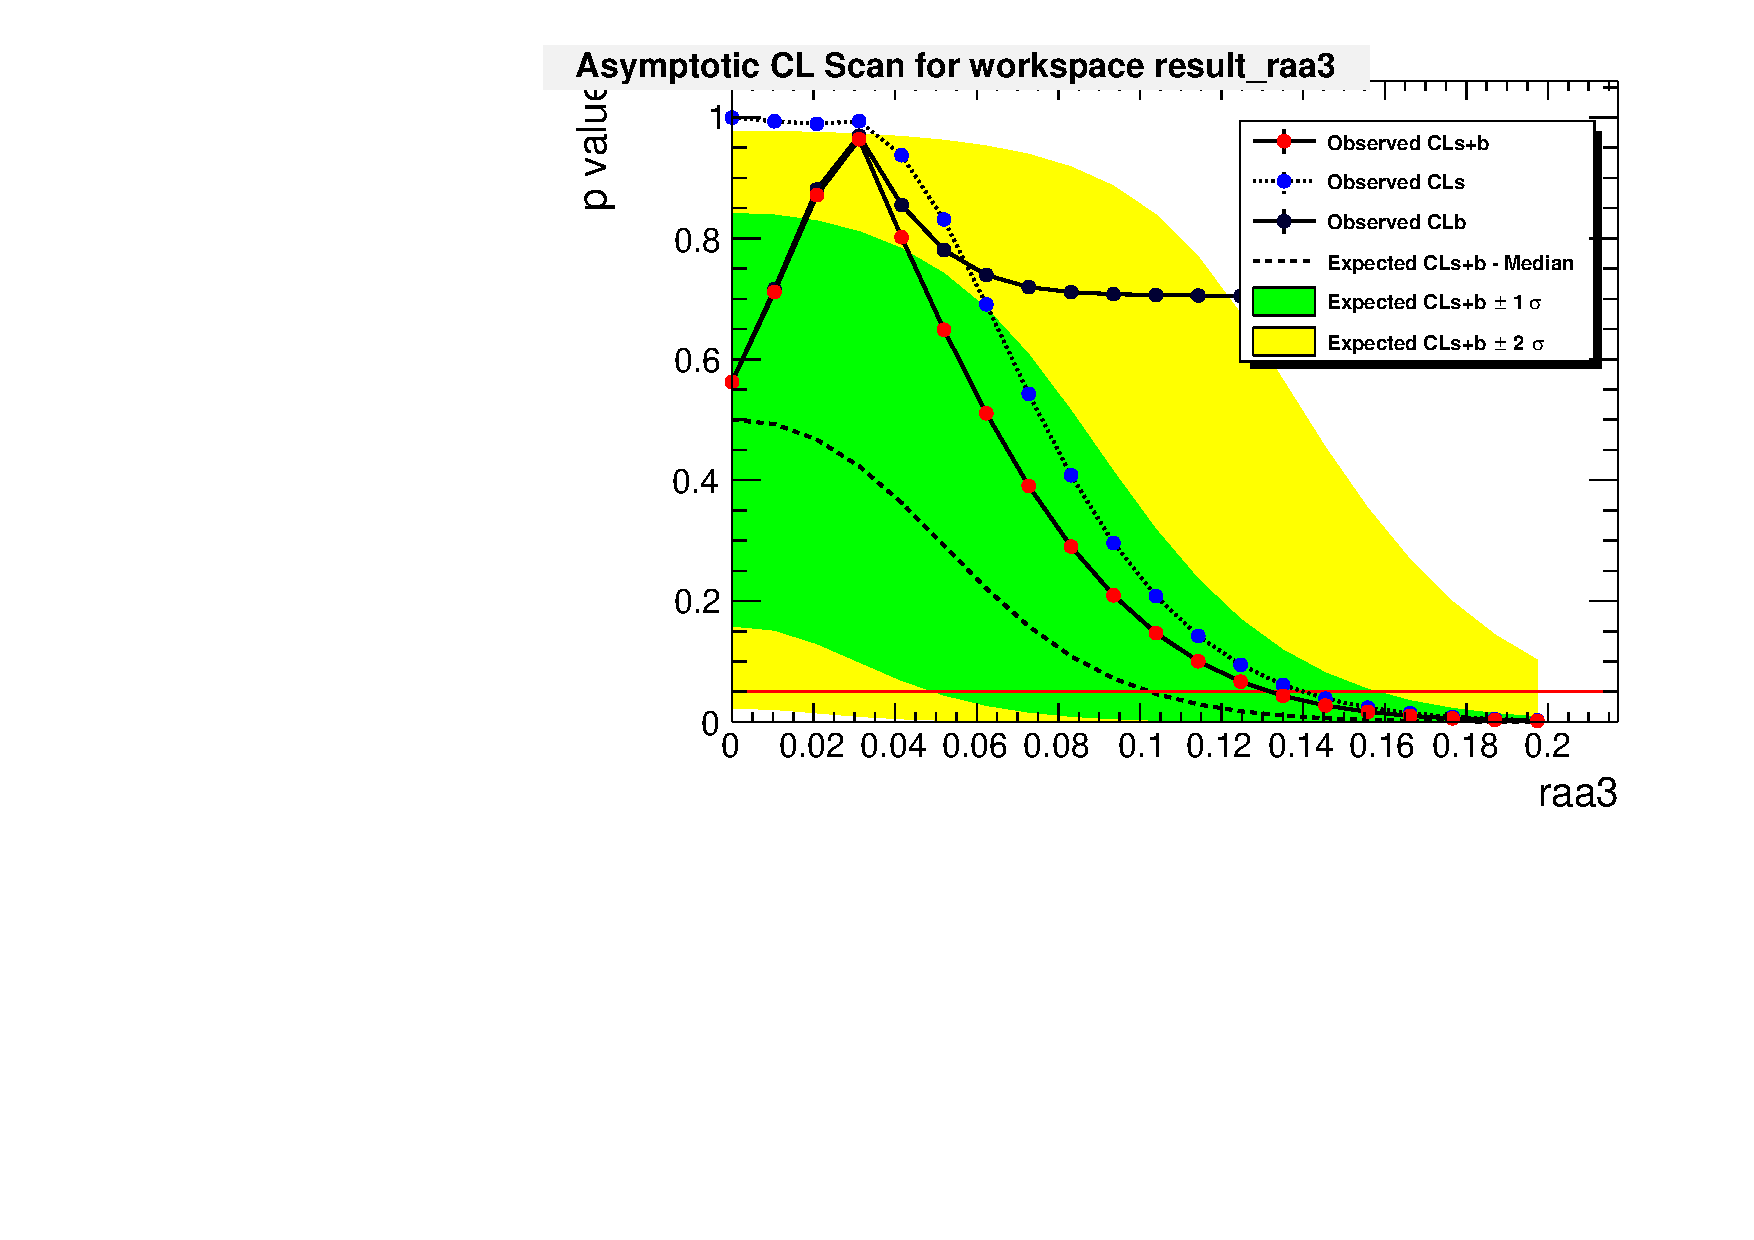
\includegraphics[width=0.49\textwidth]{Chapters/aUpsilon/asymptotic_x3raw_simple.pdf}
    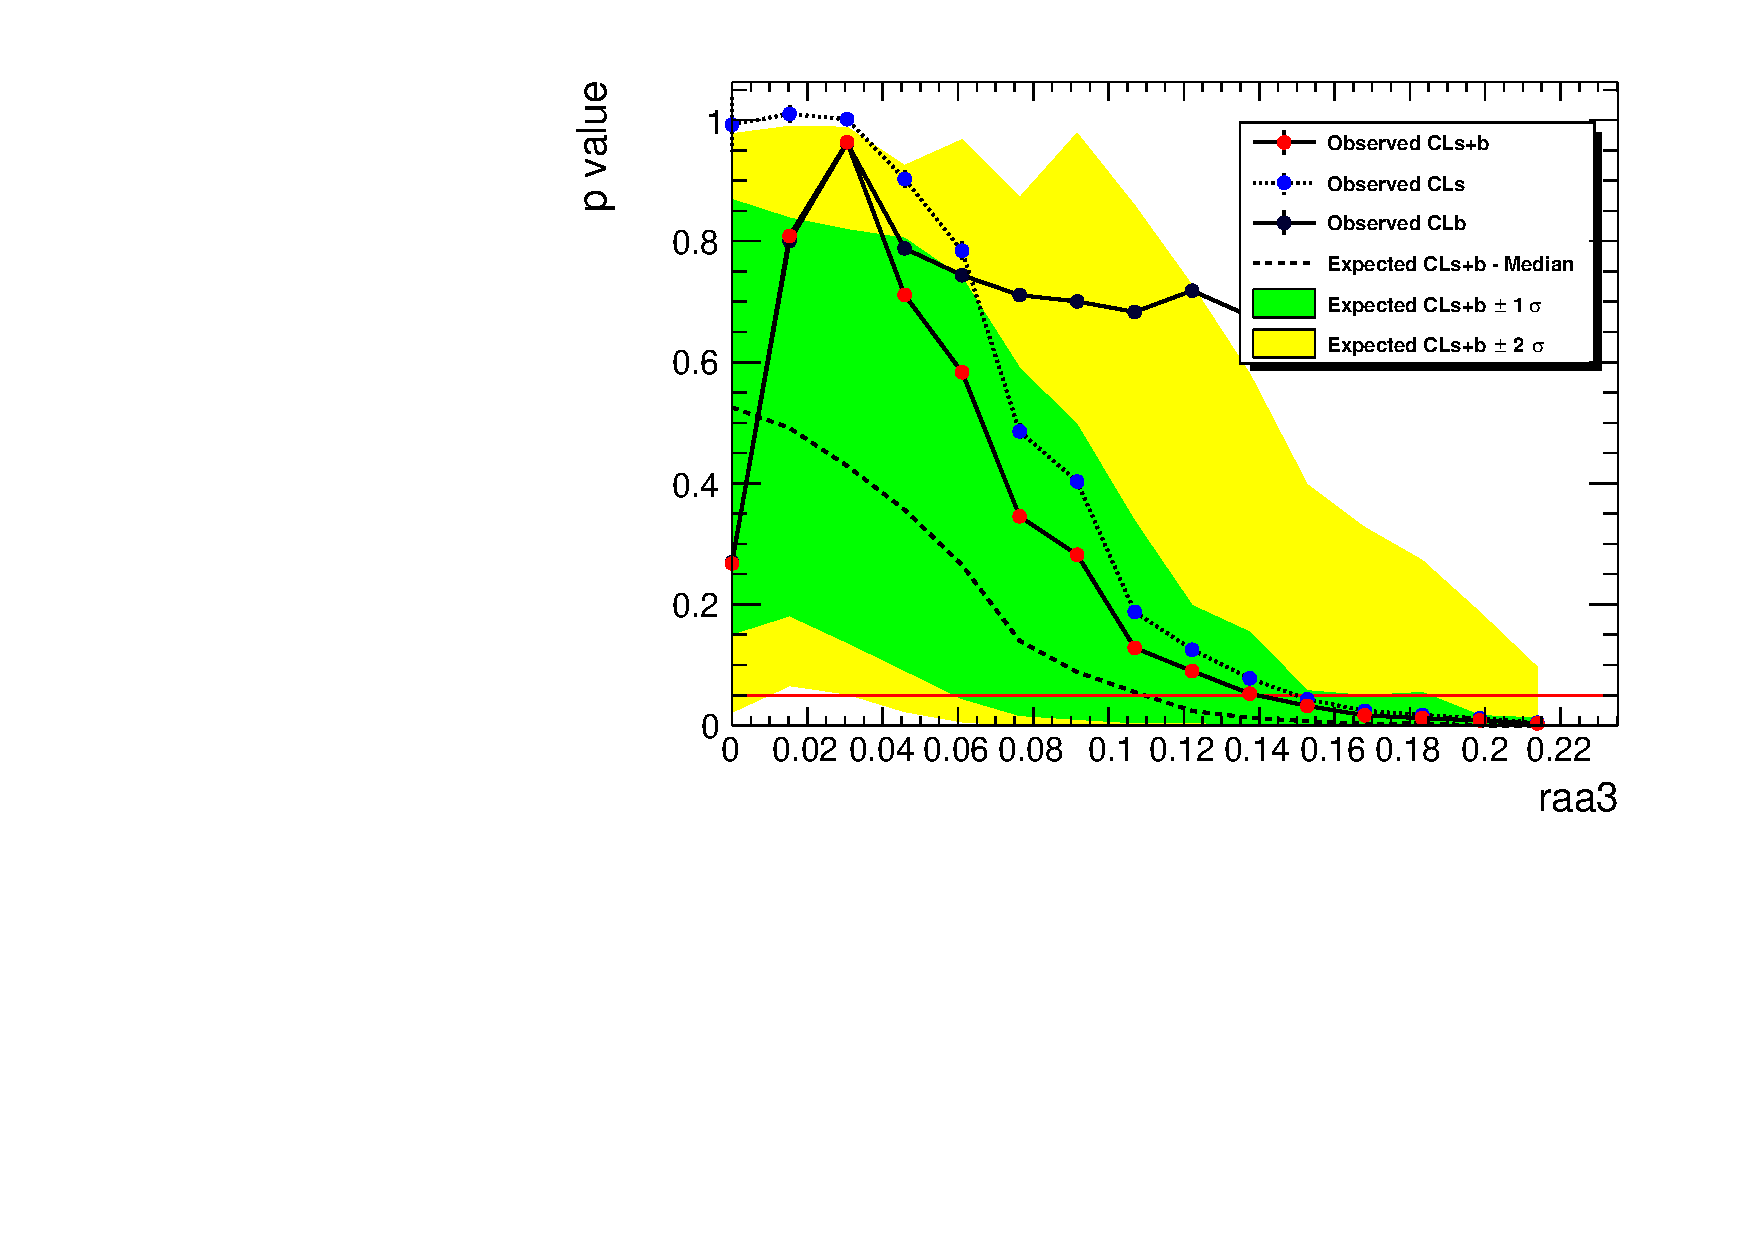
\includegraphics[width=0.49\textwidth]{Chapters/aUpsilon/frequentist_x3raw_simple.pdf}
    \caption{Asymptotic scan (left) and frequentist scan (right) of the ratio of raw 3S yields in  $pp$ and PbPb collisions, based on the Feldman and 
      Cousins approach, giving the 95\% C.L. upper limit on $\RAA(\PgUc)$.}
    \label{fig:3SUL} 
  \end{centering}
\end{figure}

\begin{figure}[h]
  \begin{centering}       
    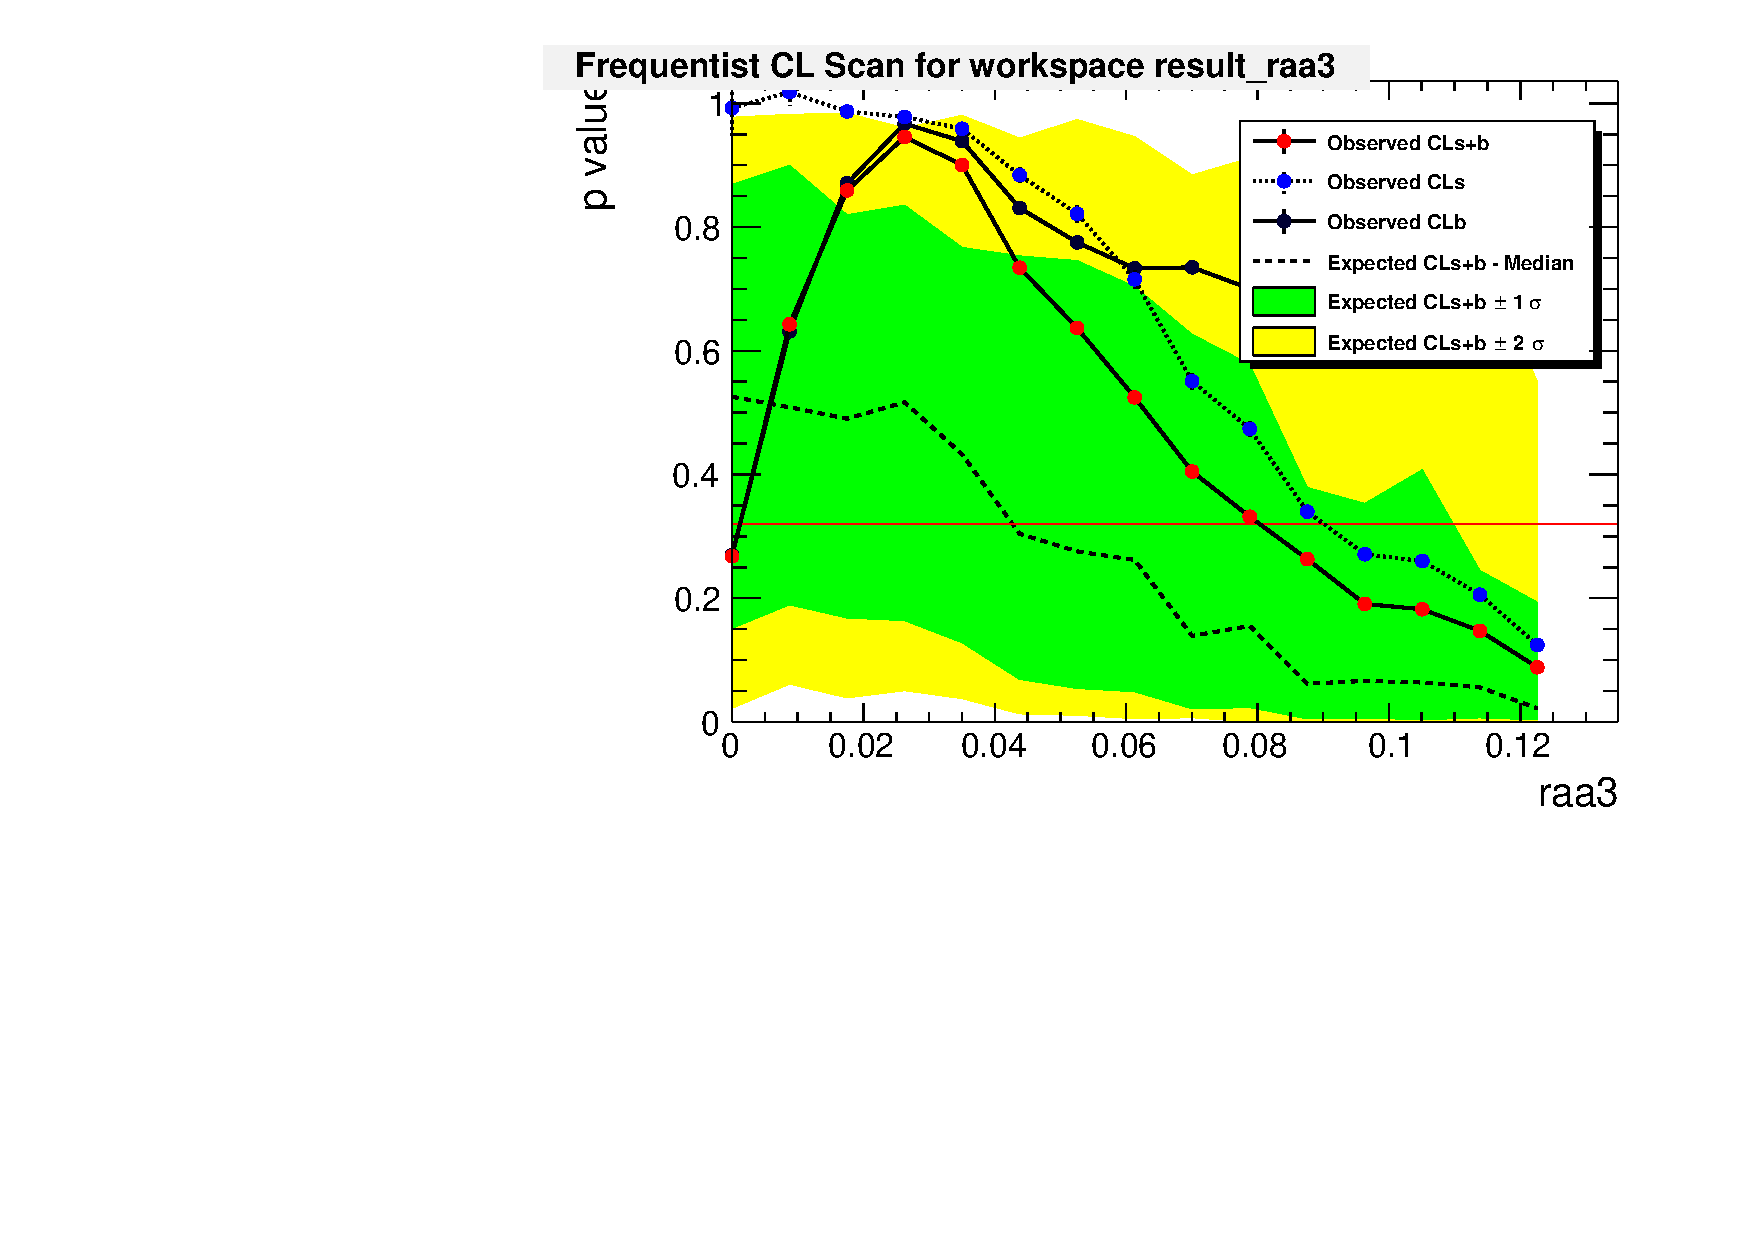
\includegraphics[width=0.49\textwidth]{Chapters/aUpsilon/frequentist_x3raw_simple_68.pdf}
    \caption{Frequentist scan of the ratio of raw 3S yields in  $pp$ and PbPb collisions, based on the Feldman and Cousins approach, giving the 68\% C.L. upper limit on $\RAA(\PgUc)$.}
    \label{fig:3SUL_68} 
  \end{centering}
\end{figure}

\vspace{0.3cm}

\fbox{
  \parbox{0.9\textwidth}
  {\textsf{The \PgUa, \PgUb\ and \PgUc\ mesons have been searched for
      in PbPb collisions, and compared to their yields in $pp$
      collisions at the same centre-of-mass energy of 2.76 \TeV\ per
      nucleon pair. The
      \PgUa\ and \PgUb\ are suppressed by a factor of $\approx 2$ and
      9, respectively, while the unobserved \PgUc\ corresponds to a
      suppression by a factor of more than 7, at the 95\% confidence
      level. Though a strong centrality dependence of the suppression
      is observed for the \PgUa\ and \PgUb\ as a function of
      centrality, no noticeable dependence is observed, neither as a
      function of transverse momentum, nor as a function of rapidity. 
      The \PgUc\ being not observed, an upper limit on its \RAA\ is
      derived, using the Feldman-Cousins prescription. The centrality
      integrated results for the nuclear modification factors of
      \PgUa, \PgUb\ and \PgUc\ are:  
      \begin{eqnarray*}
        \RAA (\PgUa) & = & 0.425 \pm 0.029~\textrm{(stat.)} \pm 0.070~\textrm{(syst.)}, \\
        \RAA (\PgUb) & = & 0.116 \pm 0.028~\textrm{(stat.)} \pm 0.022~\textrm{(syst.)}, \\
        \RAA (\PgUc) & < & 0.14 {\rm \; at \; 95\% \; CL.} 
      \end{eqnarray*}}}
}

% comparisons with other measures-> interpretation section 
\section{Discussions}
\label{sec:comparisons}
\subsection{Experimental comparisons}
The ALICE collaboration has published in 2013 in~\cite{ALICEUpsilonHI} a measurement of \PgUa\ suppression in PbPb, extending
the available \RAA\ results to the rapidity range $2.5 < y < 4$. This
publication shows a centrality integrated \RAA\ for \PgUa\ at the
value of $\RAA(\PgUa)\,=\,0.30 \pm\ 0.05~\textrm{(stat.)}~\pm\
0.04~\textrm{(syst.)}$. This result came before the present study was
made public, and in terms of CMS data, could only be compared to the
previous measurement~\cite{11-011}. The integrated result for \RAA(\PgUa) of
CMS~\cite{11-011} is compared to rapidity-dependent ALICE results
of~\cite{ALICEUpsilonHI} in
Figure~\ref{fig:alicepaper}, taken form the ALICE paper~\cite{ALICEUpsilonHI}.
\begin{figure}[h]
  \begin{centering}  
    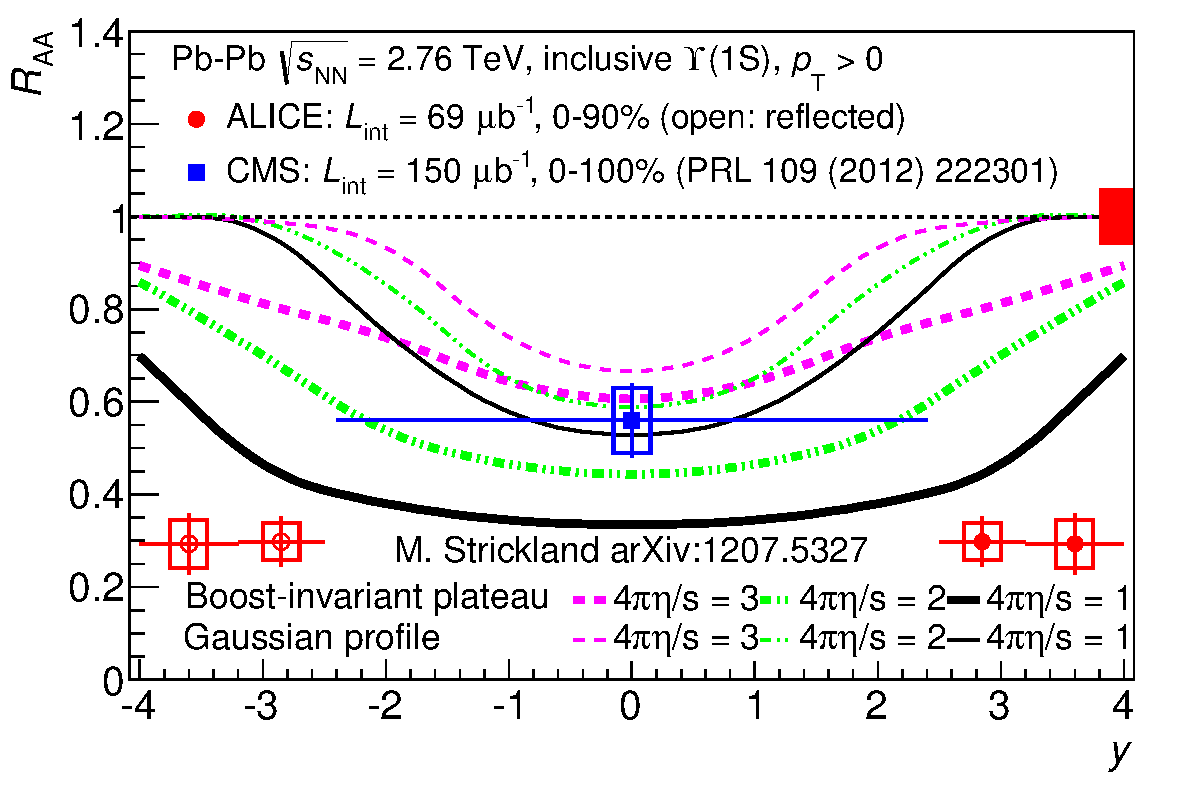
\includegraphics[width=0.8\textwidth]{Chapters/aUpsilon/Raa_th_rapidityStrick-5922.pdf}
    \caption{PbPb nuclear modification factor \RAA\ in PbPb collisions
    at \snn\ = 2.76 \TeV, as a function of \PgU\ rapidity, taken
    from~\cite{ALICEUpsilonHI}. Data from CMS publication using 2010
    $pp$ data~\cite{11-011} and ALICE~\cite{ALICEUpsilonHI}. The data
    is plotted against a potential model for quarkonium suppression
    described in~\cite{Strickland:2012cq}.}
    \label{fig:alicepaper}
  \end{centering}  
\end{figure}

Visually, the plot suggest a stronger suppression at forward
rapidities, i.e. in the acceptance of the ALICE spectrometer.
 The centrality integrated \RAA\ obtained by CMS (with
the smaller $pp$ dataset taken in 2010) was $\RAA(\PgUa)\,=\,0.56 \pm\ 0.08~\textrm{(stat.)}~\pm\
0.07~\textrm{syst.}$. Since the ALICE and CMS make independent
measurements of the \PgUa\ suppression, one can write a weighted sum
of squared errors:
\begin{equation}
\label{eq:chi2}
\chi^{2} =
\frac{\left(0.56-0.30\right)^{2}}{0.08^{2}+0.07^{2}+0.05^{2}+0.04^{2}}
\;=\;4.60 \: .
\end{equation} For this $\chi^{2}$ there is a 3.20\%
probability that another measurement yields an observed $\chi^{2}$ at
least as large~\cite{root-chi2}. This holds even if the hypothesis of no additional
suppression in ALICE data was correct (in which case, one of the
experiments just got unlucky). Assuming all the uncertainties are
normally distributed, this translates into a deviation of only 2.1 sigmas
between the two measurements. Hence, the claim in~\cite{ALICEUpsilonHI} that the data observed in
ALICE and CMS showed a rapidity dependent \PgUa\ suppression is not
statistically significant. However, the larger statistics of the
measurement presented here could allow a more stringent test for this hypothesis.



The latest \RAA(\PgUa) of CMS and ALICE data are displayed as a function of
rapidity in Figure~\ref{fig:ALICE_CMS_rap}. There is no strong \RAA\
dependence on the rapidity range considered. Indeed, using the new
integrated result $\RAA(\PgUa)\,=\,0.425 \pm\ 0.029~\textrm{(stat.)}~\pm\
0.070~\textrm{syst.}$ and applying the same chi-square test as in
Equation~\ref{eq:chi2}, one obtains a 1.3-sigma deviation between the
two integrated results. Given that the CMS result is still at the
preliminary stage and final systematic uncertainties may be reduced,
one should be cautious as with the significance computed here, as it
may change again. As a quick example of an extreme case, assuming infinite
precision in the final CMS result (with the same central value, i.e. turning the CMS uncertainties to zero in Equation~\ref{eq:chi2})
would yield a 2 sigma deviation from the 'flat suppression' hypothesis. 
\begin{figure}[h]
  \begin{centering}  
    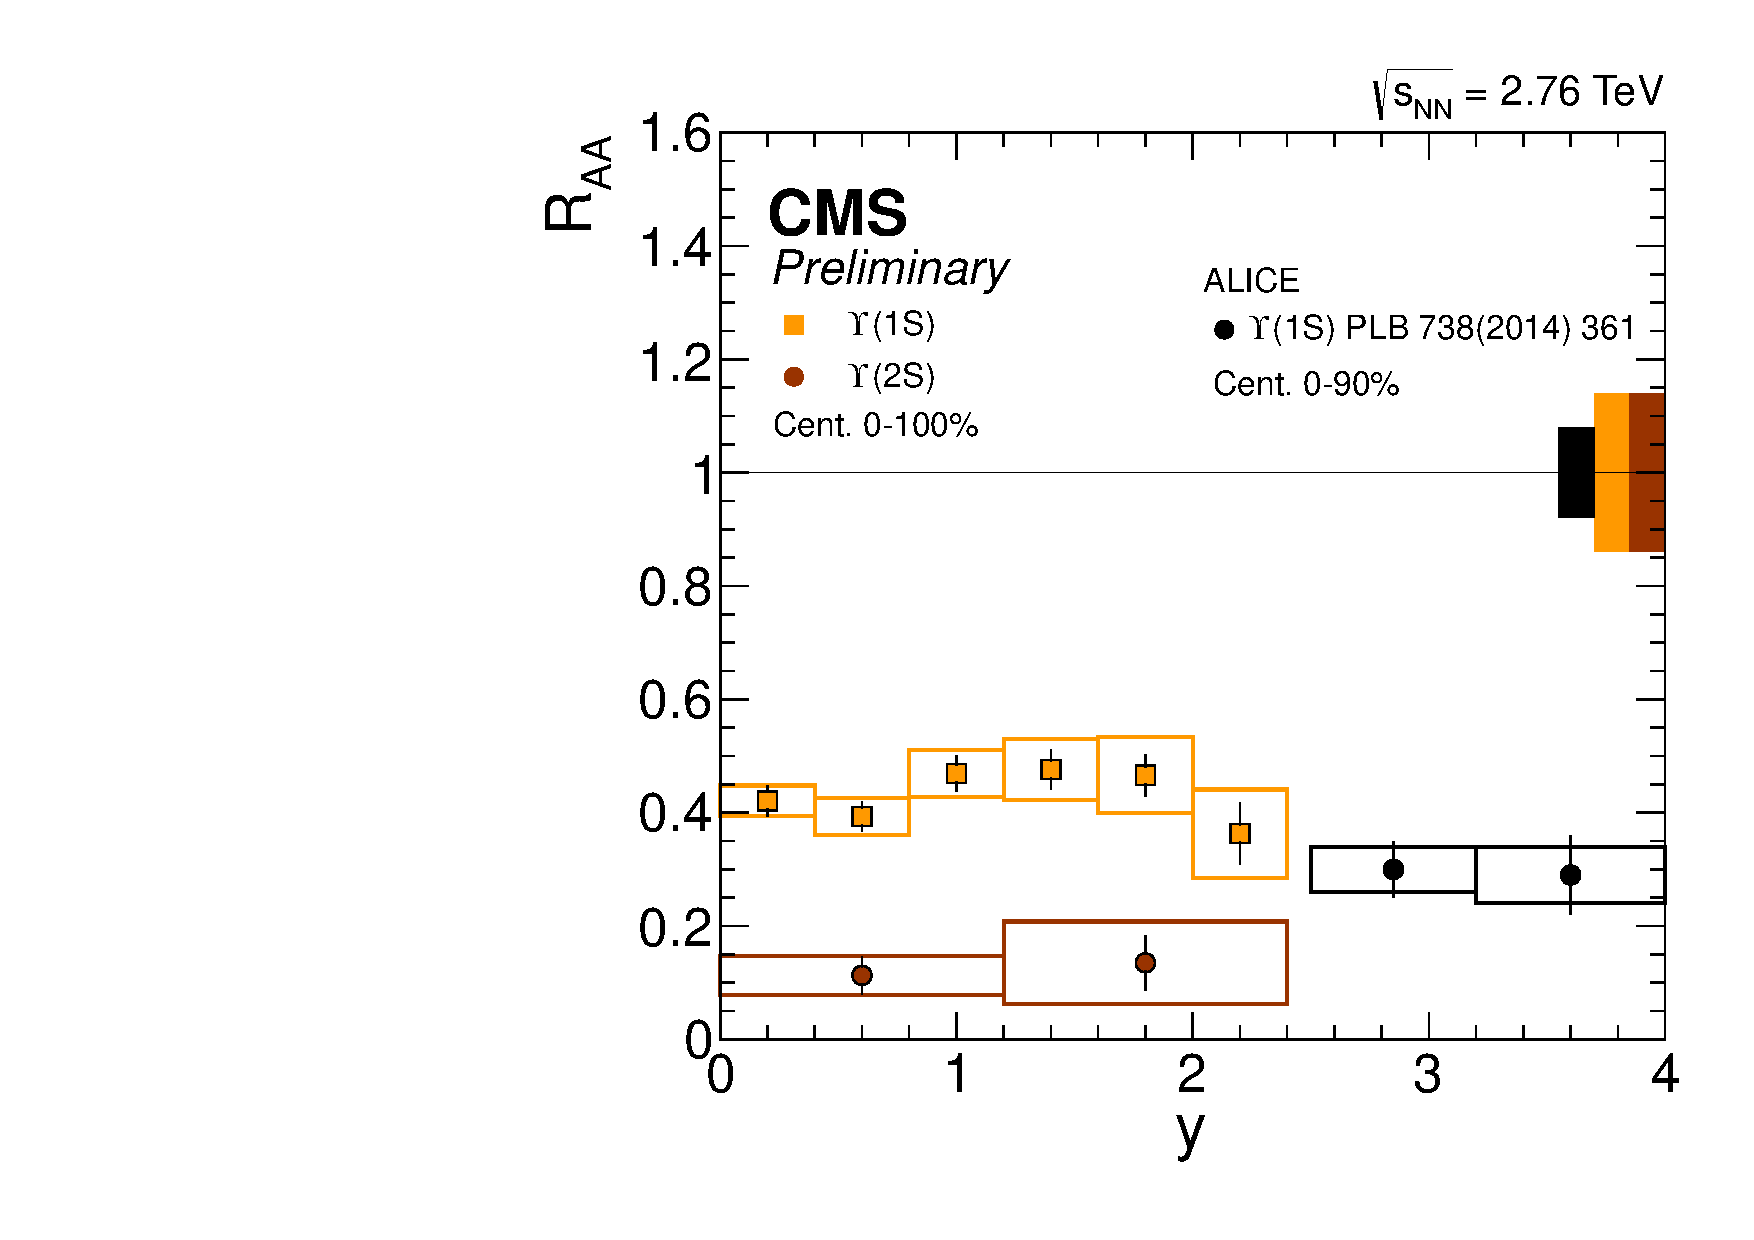
\includegraphics[width=0.75\textwidth]{Chapters/aUpsilon/ALICE_CMS_rapidity.pdf}
    \caption{PbPb nuclear modification factor \RAA\ in PbPb collisions
    at \snn\ = 2.76 \TeV, as a function of \PgU\ rapidity. Data from CMS and ALICE~\cite{ALICEUpsilonHI}.}
    \label{fig:ALICE_CMS_rap}
  \end{centering}  
\end{figure}

% A depletion of the nuclear absorption factor at forward rapidities would also be compatible with the presence of nuclear shadowing.

% From the same measurement, one can also compare the measured \RAA\ as a function of centrality. The ALICE and CMS data
% are overlaid on Figure~\ref{fig:ALICE_CMS_cent}.

% \begin{figure}[h]
%   \begin{centering}  
%     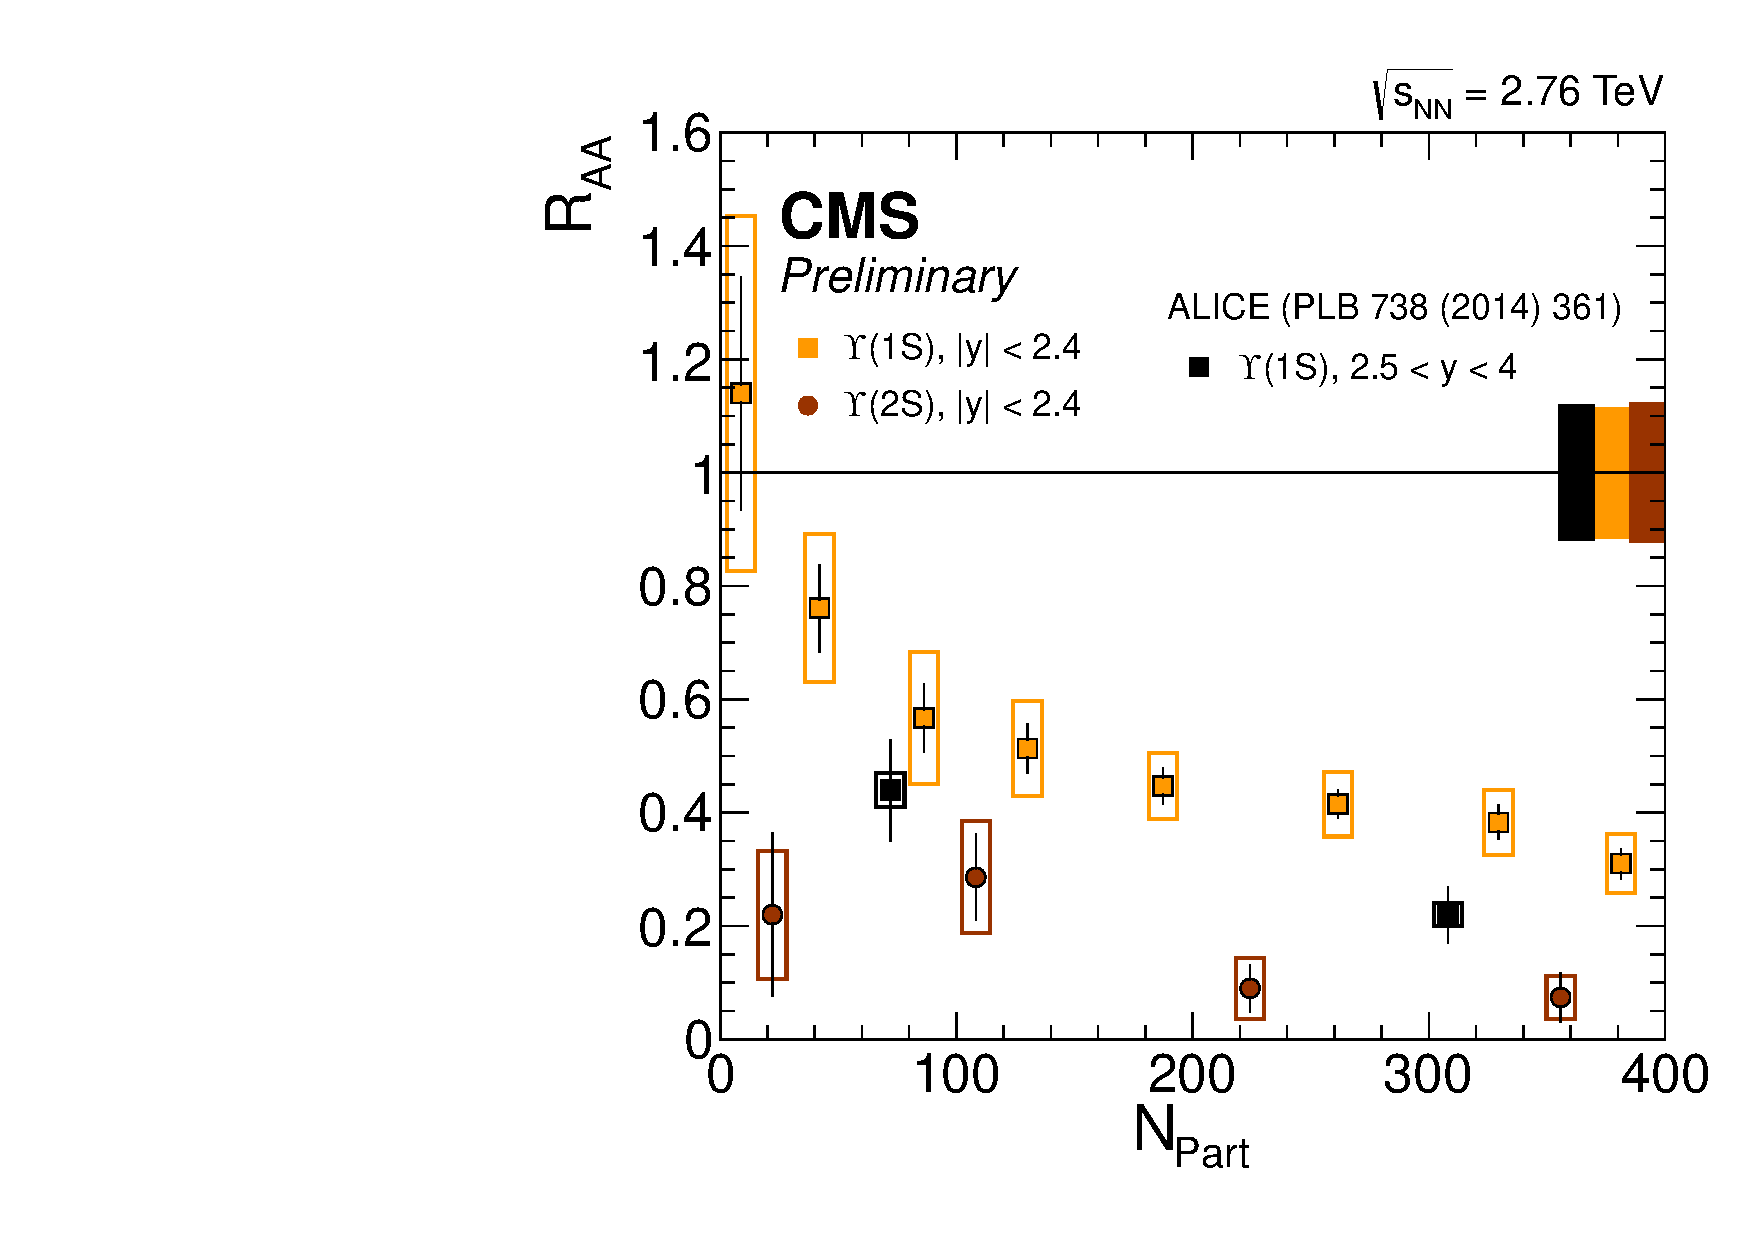
\includegraphics[width=0.75\textwidth]{Chapters/aUpsilon/CMS_ALICE_npart.pdf}
%     \caption{PbPb nuclear modification factor \RAA\ in PbPb collisions
%     at \snn\ = 2.76 \TeV, as a function of the number of participating nucleons. Data from CMS and
%     ALICE~\cite{ALICEUpsilonHI}. ALICE data is gathered in centrality bins [0-20\%], [20-90\%].}
%     \label{fig:ALICE_CMS_cent}
%   \end{centering}  
% \end{figure}

% The suppression seen in ALICE data available for \PgUa\ appears more suppressed in the centrality region 0$-$20\% than
% what is seen by CMS. This region (the most central ALICE point) should be compared to the three most central CMS
% points. On the other hand, the 20$-$90\% ALICE point should be compared to the five other CMS points (below \Npart =
% 200).


% In the case of the central points, it should be noted that the difference between CMS and ALICE points seems to be
% slightly more significant than the difference between peripheral CMS and ALICE points. 

RHIC uses gold nuclei (A = 197) while LHC uses lead nuclei
(A = 208). Comparing RHIC energies with LHC energies results in a
factor 14 increase in \snn. However, an increase of a factor 14 in
\snn\ does not change dramatically the QGP properties (i.e. the energy
density). Indeed, the charged particle multiplicity per colliding
nucleon pair measured by ALICE~\cite{Aamodt:2010cz} and
CMS~\cite{pbpbmult} in PbPb collisions at \snn\ = 2.76 TeV for the most
central collisions is about three times that measured at
PHENIX~\cite{Adler:2004zn} and PHOBOS~\cite{Alver:2010ck} at RHIC in
AuAu collisions at \snn\ = 200 GeV. In that sense, one does expect a
sizeably different \PgU\ suppression at LHC and RHIC, however not as
large as the increase in center of mass energy.

 The CMS \PgU\ data of the present analysis can be compared to RHIC
 data in a similar rapidity range: the STAR Collaboration has
 published in~\cite{Adamczyk:2013poh} a AuAu measurement of \PgU\
 suppression at \snn\ = 200 \GeV, exhibiting a lesser
 suppression at equivalent \Npart. It is exciting to see that
 recently, this AuAu data has been supplemented by reports of a
 slightly more pronounced \PgU\ suppression in UU data at the same energy,
 involving a larger number of participants than in
 AuAu~\cite{vertesi}. The suppression seen in AuAu and UU by the STAR
 experiment is compared as a function of \Npart\ in
 Figure~\ref{fig:CMS_STAR_npart}.
% \subsection{Comparisons with phenomenological models}
% \subsection{\texorpdfstring{\PgU}{Y} suppression in other
%   experiments}
\begin{figure}[h]
  \begin{centering}  
    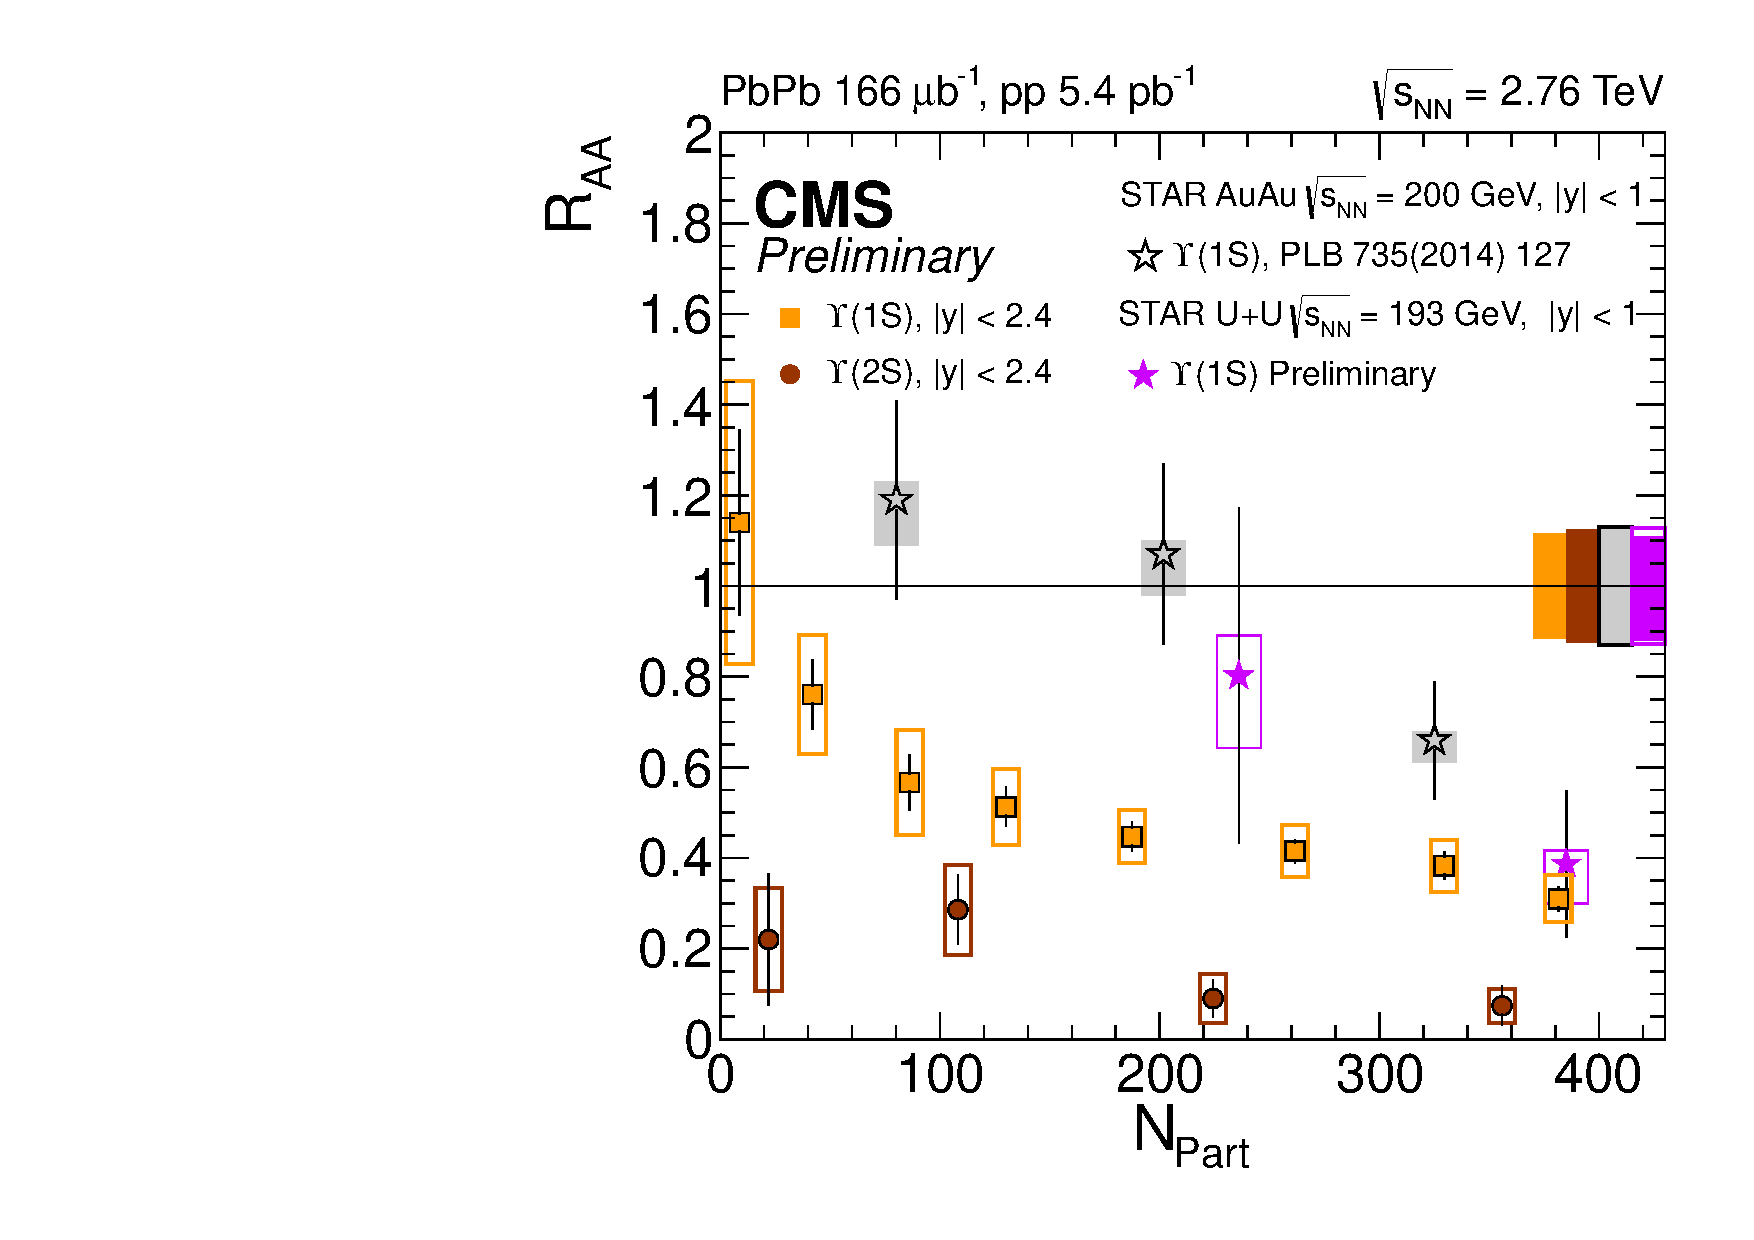
\includegraphics[width=0.75\textwidth]{Chapters/aUpsilon/CMS_STAR_npart.pdf}
    \caption{PbPb nuclear modification factor \RAA\ as a function of the number of participating nucleons. Data from CMS and
    STAR~\cite{Adamczyk:2013poh, vertesi} in AuAu and UU at \snn\ = 200 \GeV\ and 193 \GeV, respectively. ALICE data is gathered in centrality bins [0-20\%], [20-90\%].}
    \label{fig:CMS_STAR_npart}
  \end{centering}  
\end{figure}

 Within large uncertainties, the
 suppression seen by the STAR collaboration in the most central point
 (the 10\% most central UU events) finds close compatibility with
 several high-\Npart\ CMS points, from \Npart\ = 200 and
 above. Additionally, the suppression seen in 
 STAR at \Npart~$\sim$ 200 is about the same as what is reported by CMS in
 the most peripheral bin. These two observations are giving
 interesting insight on the evolution of the QGP-induced suppression with
 higher energy densities, and should be investigated further: for
 example, additional dAu data at RHIC would help to clarify the effect of
 cold nuclear matter on \PgU\ production at RHIC energies. Indeed,
 this is at the moment subject to large
 uncertainties~\cite{Adamczyk:2013poh}. Additionally, one can wonder
 what is the status of
 excited state suppression at RHIC. Since the onset of \PgUa\
 suppression is visible in RHIC data in more central events than in
 LHC data (because the energy density is smaller at RHIC than at LHC
 for a given \Npart), the suppression of \PgUb, \PgUc\ should also be
 'shifted' to higher energy densities.


So far, we are still lacking a comparison with another experiment for
our new \RAA(\PgU) result as a function of \pt. Keeping in mind that
the bottomonium and charmonium families have quite different masses,
hence different $Q^{2}$, one could compare the \pt-dependence of the
suppression seen in inclusive \Jpsi\ events recorded with
ALICE~\cite{jpsiALICE} with the flat suppression seen in our \PgU\
measurement. This comparison is shown
in~\ref{fig:ALICE_CMS_pt_psi_HIN12014}, and can be extended to higher
charmonium \pt\ using the CMS results of~\cite{12014}.


\begin{figure}[h]
  \begin{centering}  
    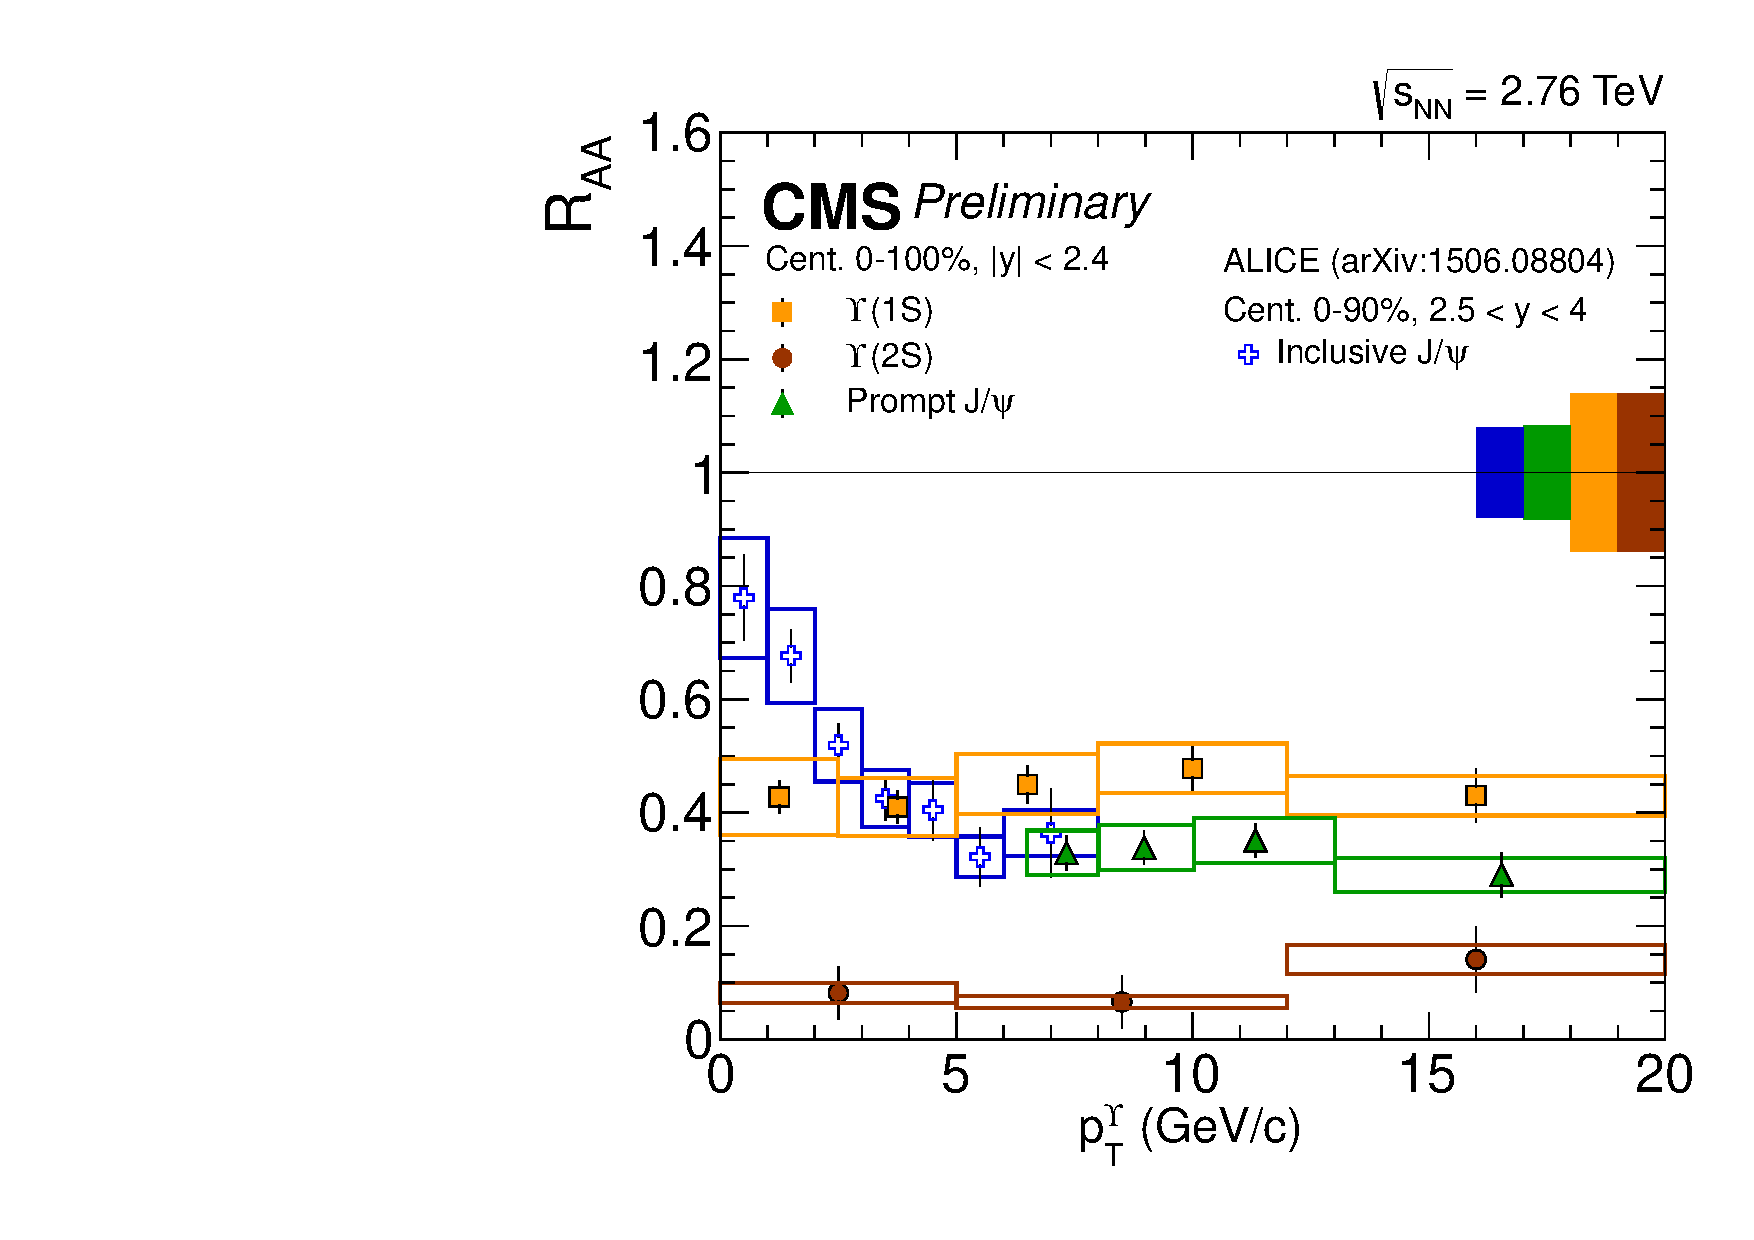
\includegraphics[width=0.75\textwidth]{Chapters/aUpsilon/ALICE_CMS_pt_psi_HIN12014.pdf}
    \caption{Comparison of the \PgUa, \PgUb\ and \Jpsi nuclear modification factors in the CMS measurement~\cite{12014} and
      with ALICE inclusive \Jpsi data from~\cite{jpsiALICE}, as a function of transverse momentum.}
    \label{fig:ALICE_CMS_pt_psi_HIN12014}
  \end{centering}  
\end{figure}


It is interesting to see that \Jpsi\ and \PgU\ seem to behave very
differently at low momenta at the LHC. At high-\pt\, the suppression is
independent of \pt\ for both species. When reducing the \pt\ of the
quarkonium pair, the suppression remains about the same for the \PgU\ family, as
we have seen. However, the suppression for \Jpsi\ starts to diminish
at $\pt(\Jpsi) \sim\ m_{\Jpsi}$. This observation could be considered
as an indirect confirmation of a sizeable regeneration mechansism in the charmonium spectrum at low-\pt, setting off
as the momentum increases. 


% The \Jpsi data of
% ALICE and CMS~\cite{12014} is compared to \PgU\ measurements in rapidity and \pt\ on Figures~\ref{fig:ALICE_CMS_rapidity_psi}
% and~\ref{fig:ALICE_CMS_pt_psi_HIN12014}, respectively.



% \begin{figure}[h]
%   \begin{centering}  
%     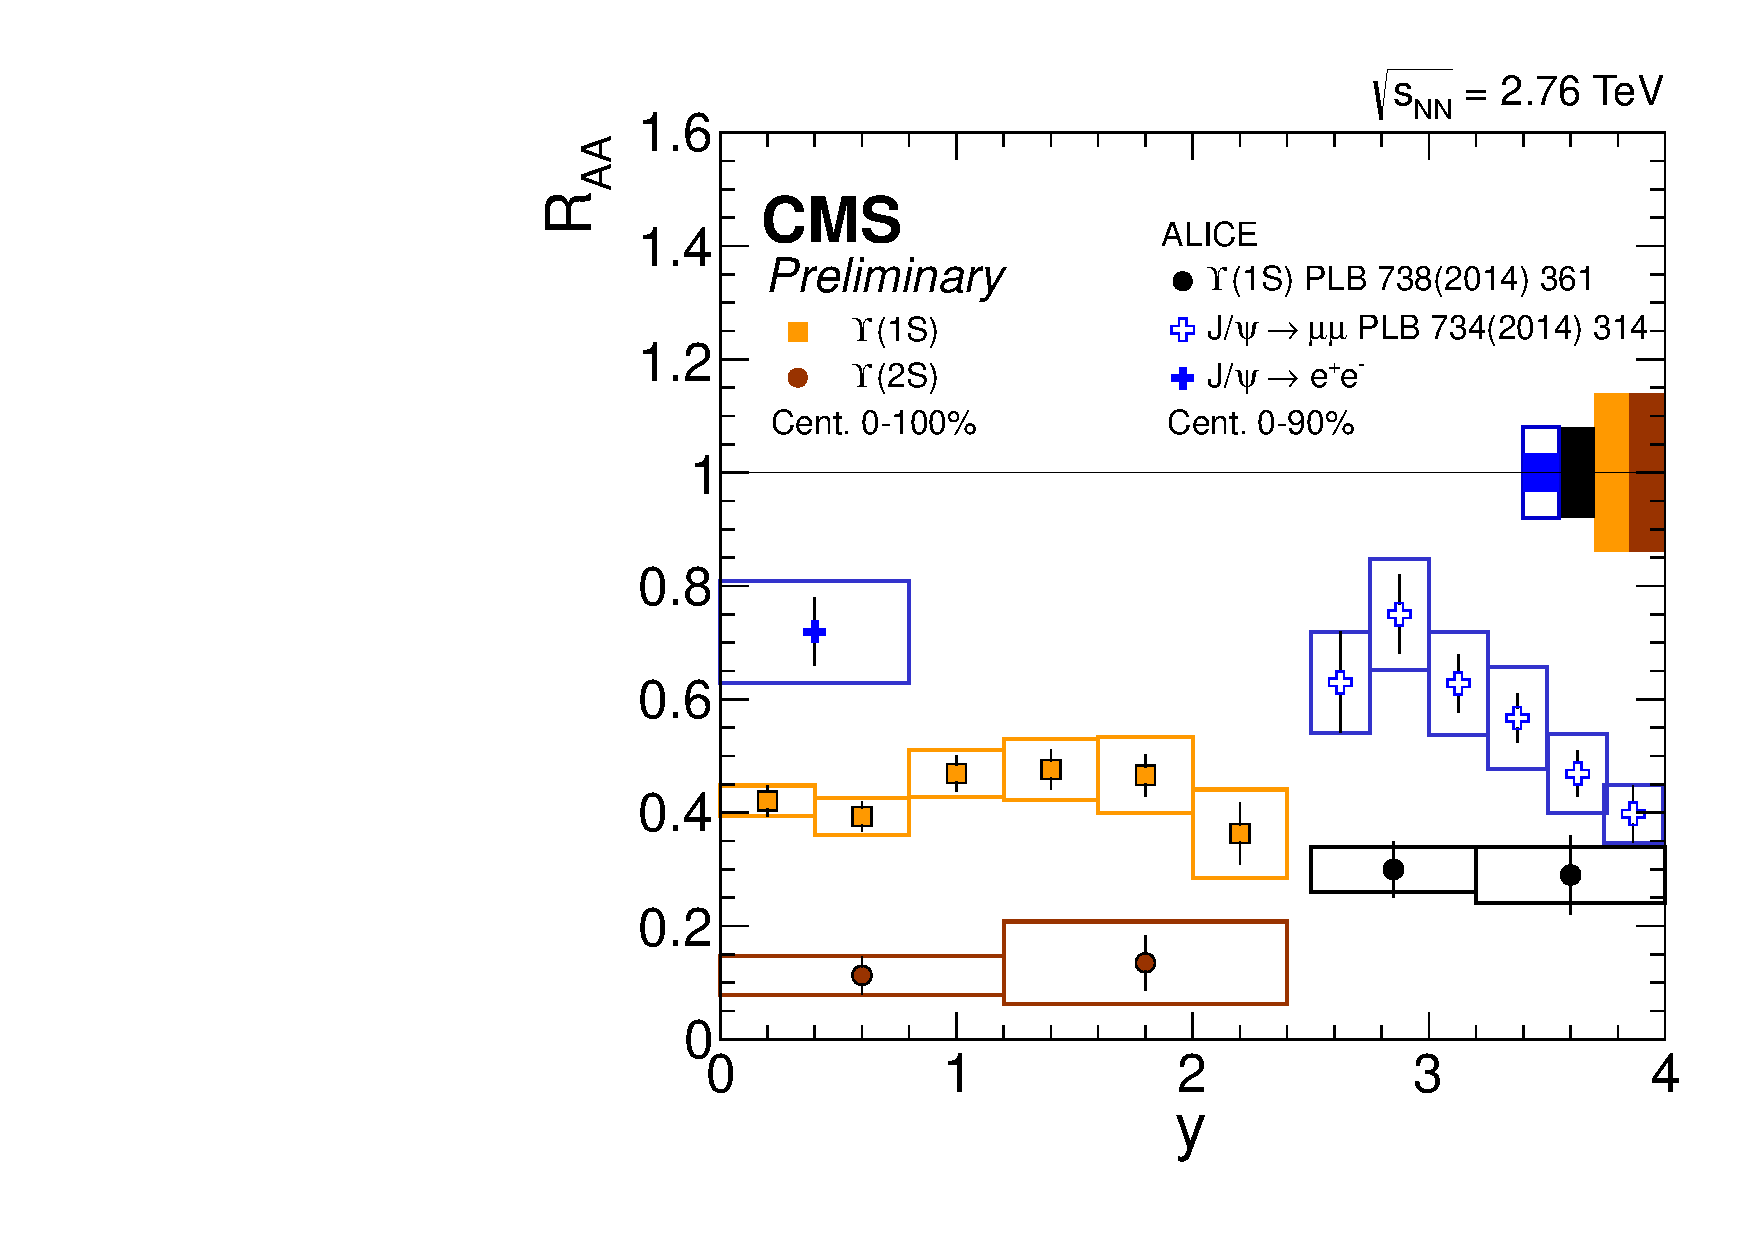
\includegraphics[width=0.75\textwidth]{Chapters/aUpsilon/ALICE_CMS_rapidity_psi.pdf}
%     \caption{Comparison of the \PgUa, \PgUb\ and \Jpsi nuclear modification factors in the CMS measurement~\cite{12014} and
%       with ALICE inclusive \Jpsi data from~\cite{jpsiALICE}, as a function of rapidity.}
%     \label{fig:ALICE_CMS_rapidity_psi}
%   \end{centering}  
% \end{figure}


Before moving to comparisons with theoretical models for \PgU\
suppression, I should discuss the impact of nuclear absorption or
other cold nuclear matter effects in all of the figures
above. Obviously, the beginning of a data-based distinction between cold and hot effects is
very difficult at this stage: the data is still quite insufficient in
peripheral events, where hot effects are not expected to
dominate. Additionally, one would need a $R_{pA}$ for individual \PgU\
at the same center of mass energy and in the same rapidity range as
the CMS measurement, to get a grasp of the cold nuclear effects due to
one heavy nucleus. The ATLAS collaboration has recently put forth a
measurement of the $p$Pb nuclear modification factor, based on an
extrapolated $pp$ cross section at \s\ = 5.02 TeV from other
energies~\cite{ATLAS-CONF-2015-050}. This interesting first attempt at
estimating the \PgUa\ cold nuclear effects in the central rapidity region
shows that they are small.

For what concerns the excited states~\PgUb\ and \PgUc, it has been
demonstrated first in~\cite{Chatrchyan:2013nza} that these suffer
slight additional modification in $p$Pb at \snn\ = 5.02 TeV, with
respect to the ground state. This modification is smaller than what is
observed in PbPb collisions at LHC energies. Additional studies of the
peripheral AA collisions, as well as pA collisions of increasing
centralities, are needed to better understand what are the various
processes at play in this regime. 

% Models of the effect of nuclear absorption,
% comovers or shadowing on quarkonia~\cite{Armesto:1997sa,Capella:1996va,Capella:2000zp,Eskola:2009uj}
% all come with an uncertainty (dependent on the source of cold nuclear
% modification), which is rather uncontrolled at high-\Npart, where hot
% effects should set in. In the event of no quarkonium melting, one
% could compare these predictions with data, as is done in $p$Pb
% collisions. This is out of the scope of this discussion, since we
% focus on results from nucleus-nucleus collisions.
%  The same applies when gluon saturation is considered. The Color Glass
%  Condensate (CGC) model proposes a nuclear modification dependent on the gluon saturation
% scale, $Q^{2}_{s}$~\cite{Fujii:2006ab}. Again, this is helpful in the
% proton-nucleus collision system, and can hardly be extrapolated to the
% nucleus-nucleus collision case.%  Moreover, the CGC calculations for
% % quarkonium production~\cite{Fujii:2006ab} make use of either N

% Finally, \Jpsi\ nuclear modification in $p$Pb data from
% ALICE~\cite{alicejpsipPb} shows a satisfactory agreement with 
%  upon the large uncertainty on gluon
% nuclear PDF. We can however judge that in the
% case of bottomonia these sources are less affecting the yield as they would
% in the case of charmonia. Additionally, the pPb data available from
% the 2013 $p$Pb run at LHC revealed a small modification of the ground
% state yield~\cite{}

% p to the most
% central PbPb the contribution is 
\subsection{Comparisons with suppression models in PbPb}

Figure~\ref{fig:RAA_TH_cent_rapp} shows a comparison of centrality binned data from CMS with the transport model of
Rapp~\textit{et al.} using a rate equation approach detailed
in~\cite{Emerick:2011xu}, and applied in the strong binding
scenario~\cite{Zhao:2011cv}. In this model, primordial and regenerated contributions are taken into
account. However, it is worth pointing out that regeneration
necessitates a large initial number of quark pairs produced. In other
words, the regeneration component is expected to depend on the total
$q\bar{q}$ production cross section. In the case
of $b\bar{b}$ it is unclear how many pairs are produced in central PbPb collisions, however the exact number should be
of the order of 5$\sim$10, preventing \PgU\ a sizeable regeneration
effect to occur at present LHC energies.
\begin{figure}[h]
  \begin{centering}  
    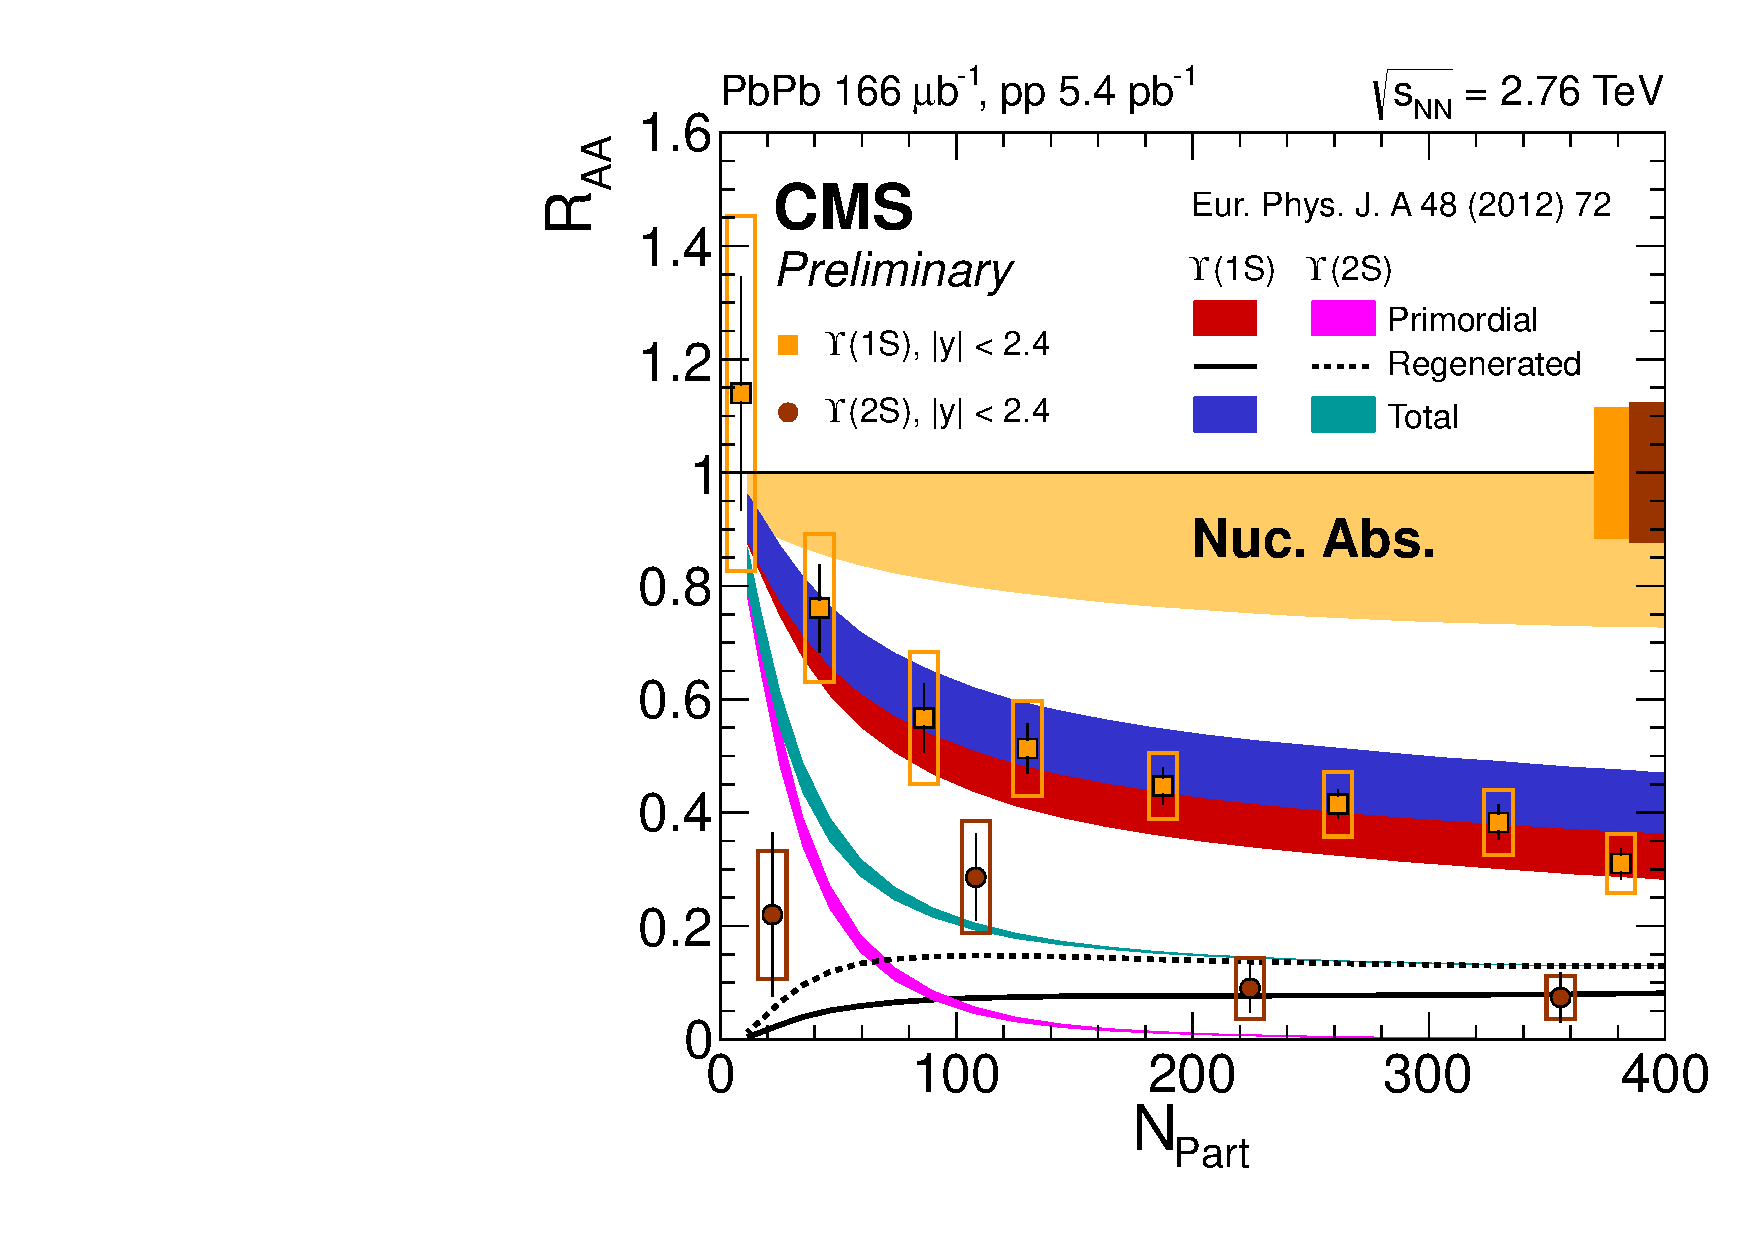
\includegraphics[width=0.65\textwidth]{Chapters/aUpsilon/RAA_NPART_Rapp.pdf}
    \caption{PbPb nuclear modification factor \RAA\ in PbPb collisions
      at \snn\ = 2.76~\TeV, as a function of the number of participants.}
    \label{fig:RAA_TH_cent_rapp}
  \end{centering}  
\end{figure}

 I have plotted the regeneration and primordial contributions on
Figure~\ref{fig:RAA_TH_cent_rapp} for completeness. The model manages
to reproduce the data. It should be pointed out
from~\cite{Zhao:2011cv} that the primordial component is constantly suppressed over the \pt\ range scanned
in~\cite{Zhao:2011cv} (computed there
for \Jpsi, not \PgU). This would suggest that a constant suppression
over \pt\ could also be expected when this model is applied to \PgU. I
am not aware of the actual calcultation leading to the amount of
nuclear absorption shown in this figure; at large \Npart, a good
fraction of the agreement between model and data could be accounted to
this contribution, which cannot be confirmed.
\begin{figure}[h]
  \begin{centering}  
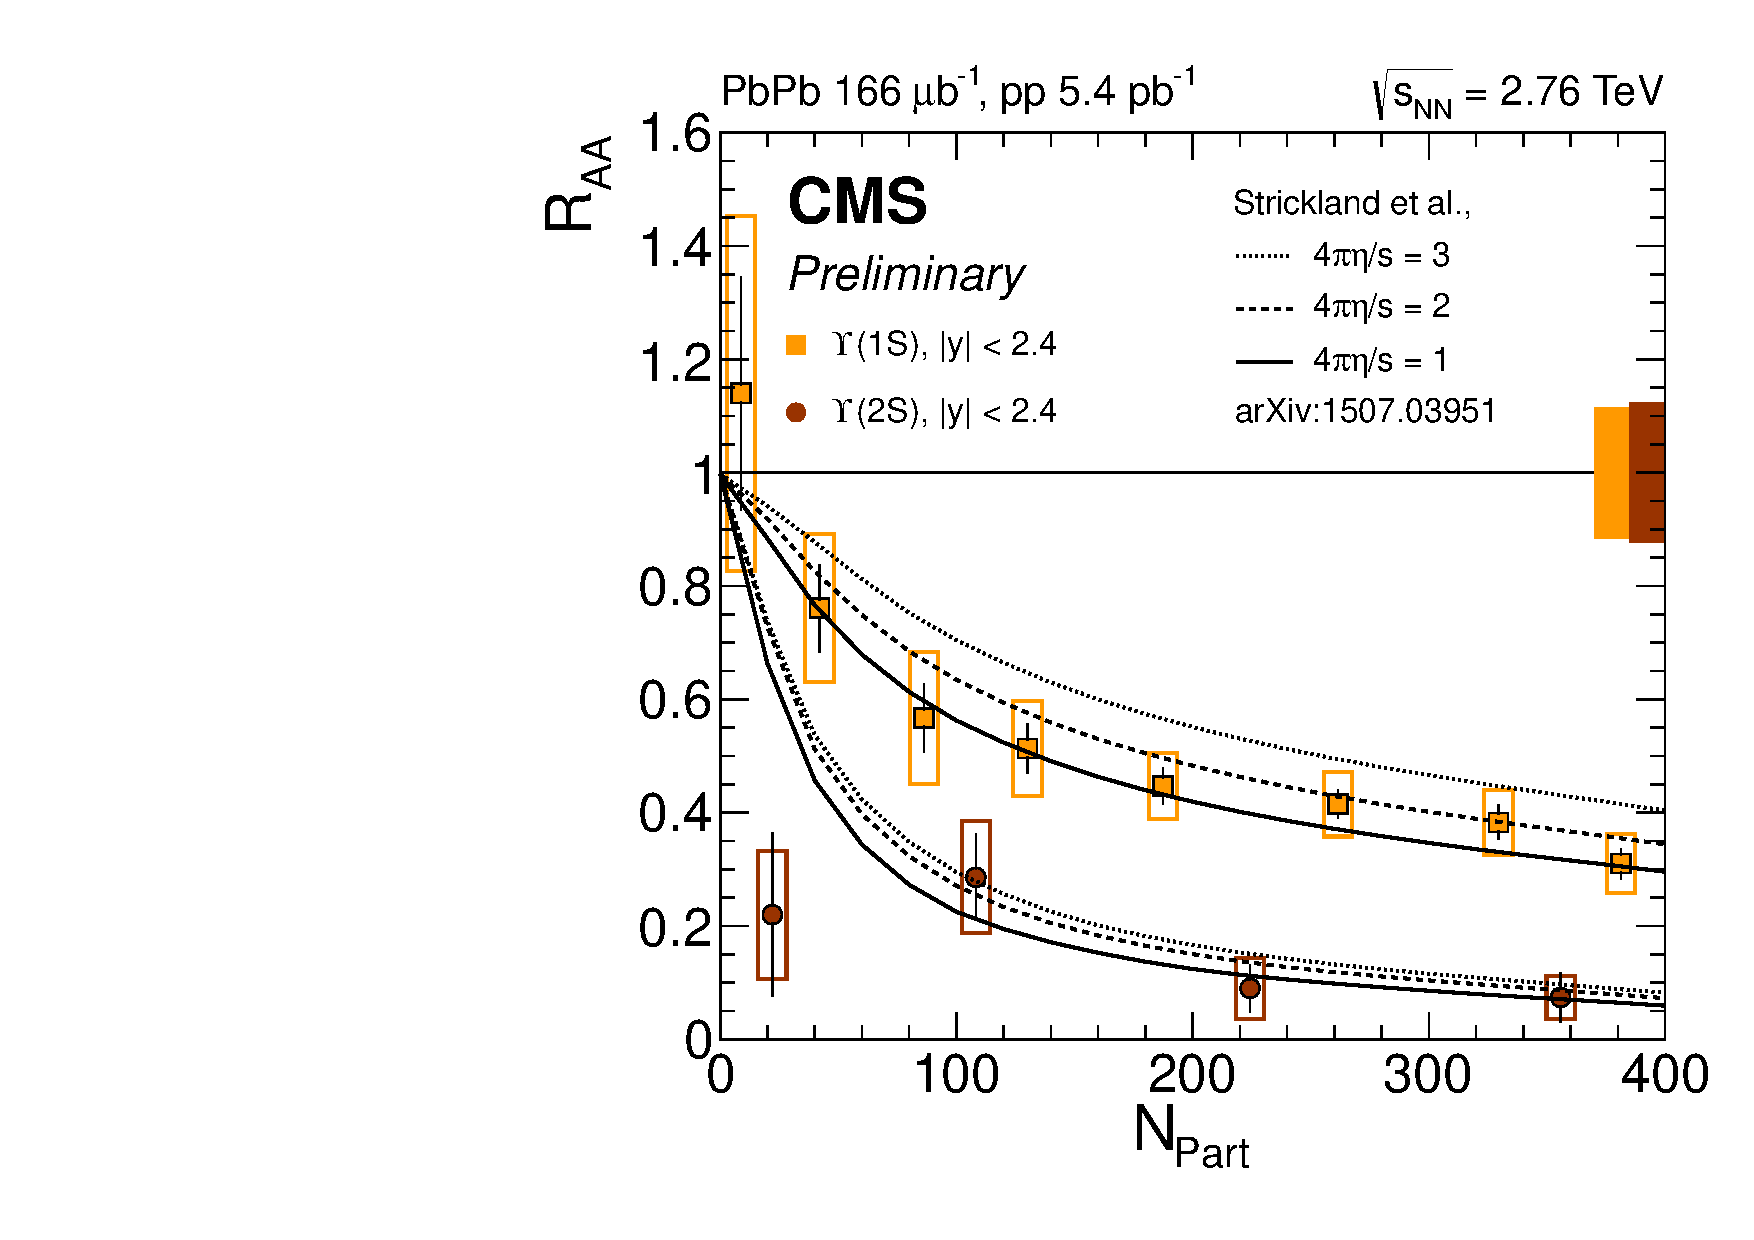
\includegraphics[width=0.65\textwidth]{Chapters/aUpsilon/RAA_NPART_Strickland.pdf}
    \caption{PbPb nuclear modification factor \RAA\ in PbPb collisions
      at \snn\ = 2.76~\TeV, as a function of the number of participants. Comparison with updated calculations from Strickland~\cite{Krouppa:2015yoa}.}
    \label{fig:RAA_TH_cent_strickland}
  \end{centering}  
\end{figure}

Figure~\ref{fig:RAA_TH_cent_strickland} shows a comparison of
centrality-binned data from CMS with a hydrodynamic model from
Strickland~\textit{et al.}~\cite{Krouppa:2015yoa}. This result is an
update of a computation using a complex-valued binding potential
for the quark pair, described in~\cite{Strickland:2012cq}. The value
of the real
part of the potential informs on the binding of the state: if
the real part is positive (negative), the quarkonium is bound
(unbound). The imaginary part of the potential gives a description of
the dissociation rate of a given state as a function of the medium
temperature. From $T\sim 250$ MeV and above, the imaginary part of the
potential is related to a Landau-damping process of the gluon fields,
which gives a decay width to the quarkonium state, as reported
in~\cite{Laine:2006ns}. The thermodynamic evolution considered here was
initially described in~\cite{Strickland:2011aa}, and accounts for large
momentum-space anisotropies in the plasma. In the version shown
in~\cite{Krouppa:2015yoa} and in Figure~\ref{fig:RAA_TH_cent_strickland},
the anisotropic hydrodynamical model accounts for transverse expansion
(3+1D dynamics) which is an improvement compared
to~\cite{Strickland:2012cq}.




The hydrodynamical treatment can be tuned to different values of the
shear viscosity to entropy ratio, $\eta/s$. The data seem to favor a
scenario where $\eta/s$ is close to 1/4$\pi\;\sim$/4$\pi$. A clear
overview of the importance of the value of $\eta/s$ in strongly
coupled theories is available in~\cite{Shuryak:2003xe}.


The same model is tested against data as a function \pt\ and $y$, in
Figures~\ref{fig:RAA_TH_kin_strickland} left and right. On the left
hand side, the \RAA\ as a function of \pt\ is presented. The model
suggest a slow reduction of the suppression factor with increasing
momentum. From this figure it is difficult to tell whether the data
would follow this slowly rising trend at higher momentum values. More
data in the forthcoming heavy ion physics runs of CMS and other LHC
experiments may shed more light on the high-\pt\ regime. On the right
hand side, the rapidity dependence of the model is tested against CMS
and ALICE \PgUa\ data from~\cite{ALICEUpsilonHI}.
\begin{figure}[h]
  \begin{centering}  
    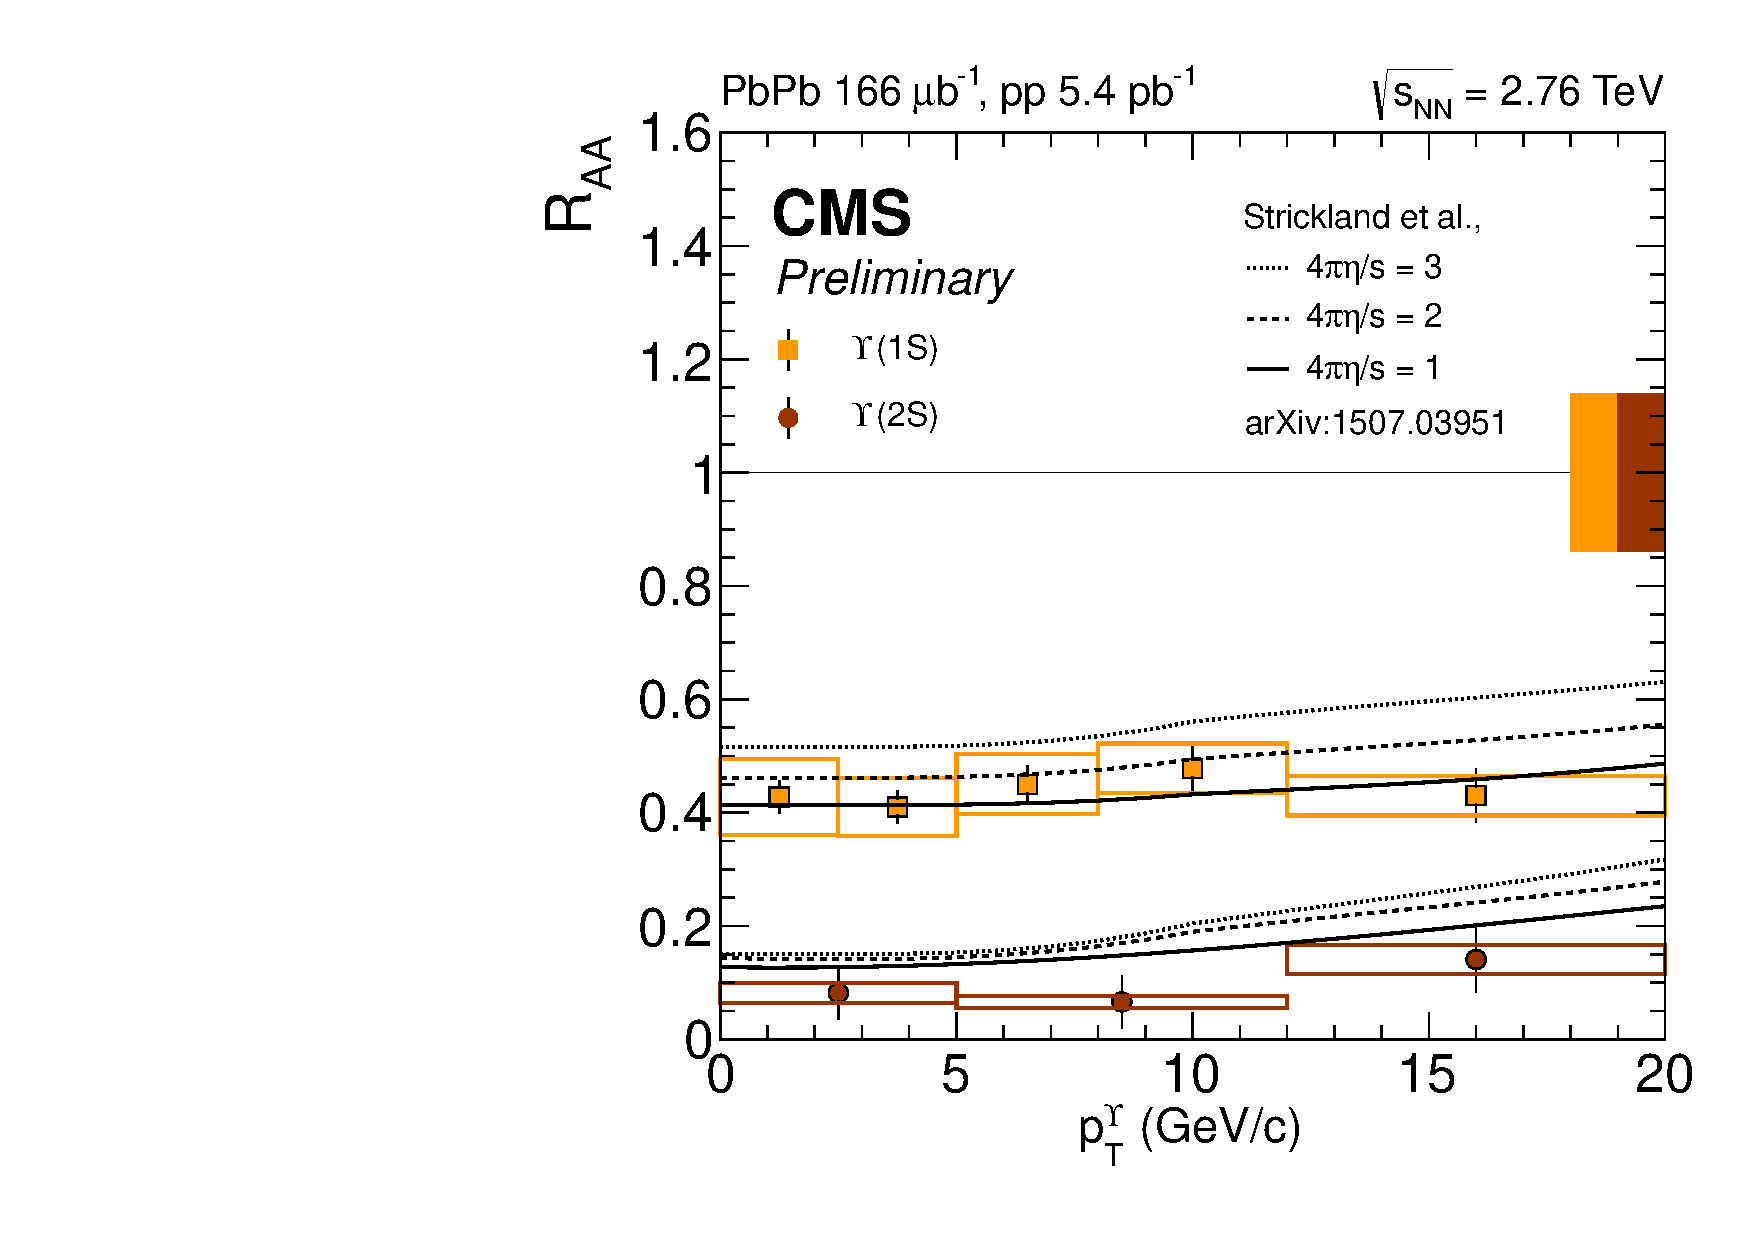
\includegraphics[width=0.7\textwidth]{Chapters/aUpsilon/RAA_PT_Strickland.pdf}
    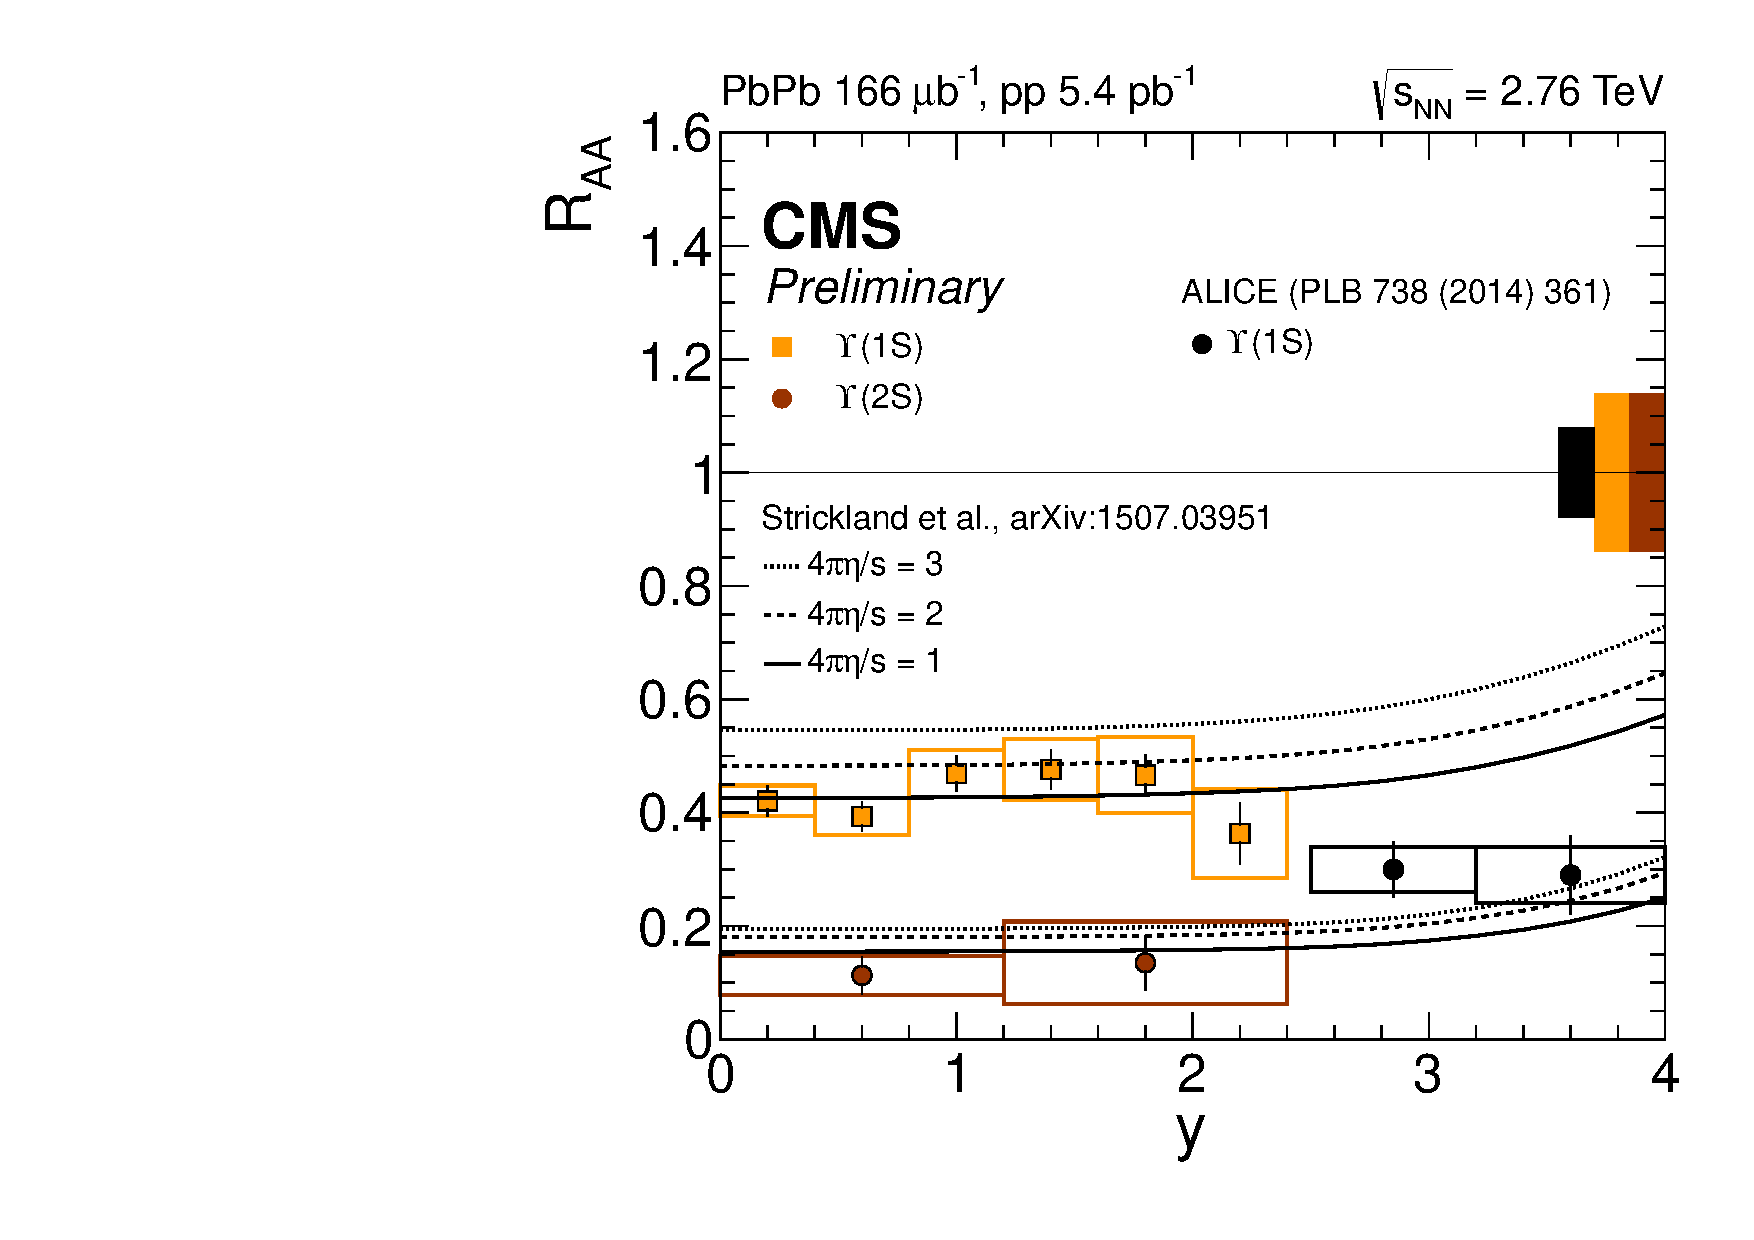
\includegraphics[width=0.7\textwidth]{Chapters/aUpsilon/RAA_RAP_Strickland_alice.pdf}
    \caption{PbPb nuclear modification factor \RAA\ in PbPb collisions
      at \snn\ = 2.76~\TeV, as a function of the \PgU\ \pt\ and \y. Theoretical curves obtained from anisotropic
      hydrodynamics from~\cite{Krouppa:2015yoa}.}
    \label{fig:RAA_TH_kin_strickland}
  \end{centering}  
\end{figure}

Some tension appears at high rapidity, where the ALICE data appears
below the expected suppression for this model. It should be noted that
this discrepancy was already visible at the beginning of this section,
in Figure~\ref{fig:alicepaper}, where the modeled \PgUa\ suppression
wore off faster at larger rapidities. The version presented in
Figures~\ref{fig:RAA_TH_kin_strickland}
and~\ref{fig:RAA_TH_cent_strickland} includes an update for how
the \PgU\ are distributed over the centrality variable. In other
words, the model benefitted of a \Ncoll-reweighting to mimick the
proper centrality distribution for hard probes (previously assuming a
flat distribution). This fix visibly reduced the discrepancy between the model
and the forward rapidity data from ALICE.%  The authors argue that additional nuclear
% absorption (presently not significant) could now be considered responsible for the  decrease of the
% \RAA(\PgUa) at forward rapidities, 
% \begin{figure}[h]
%   \begin{centering}  
%     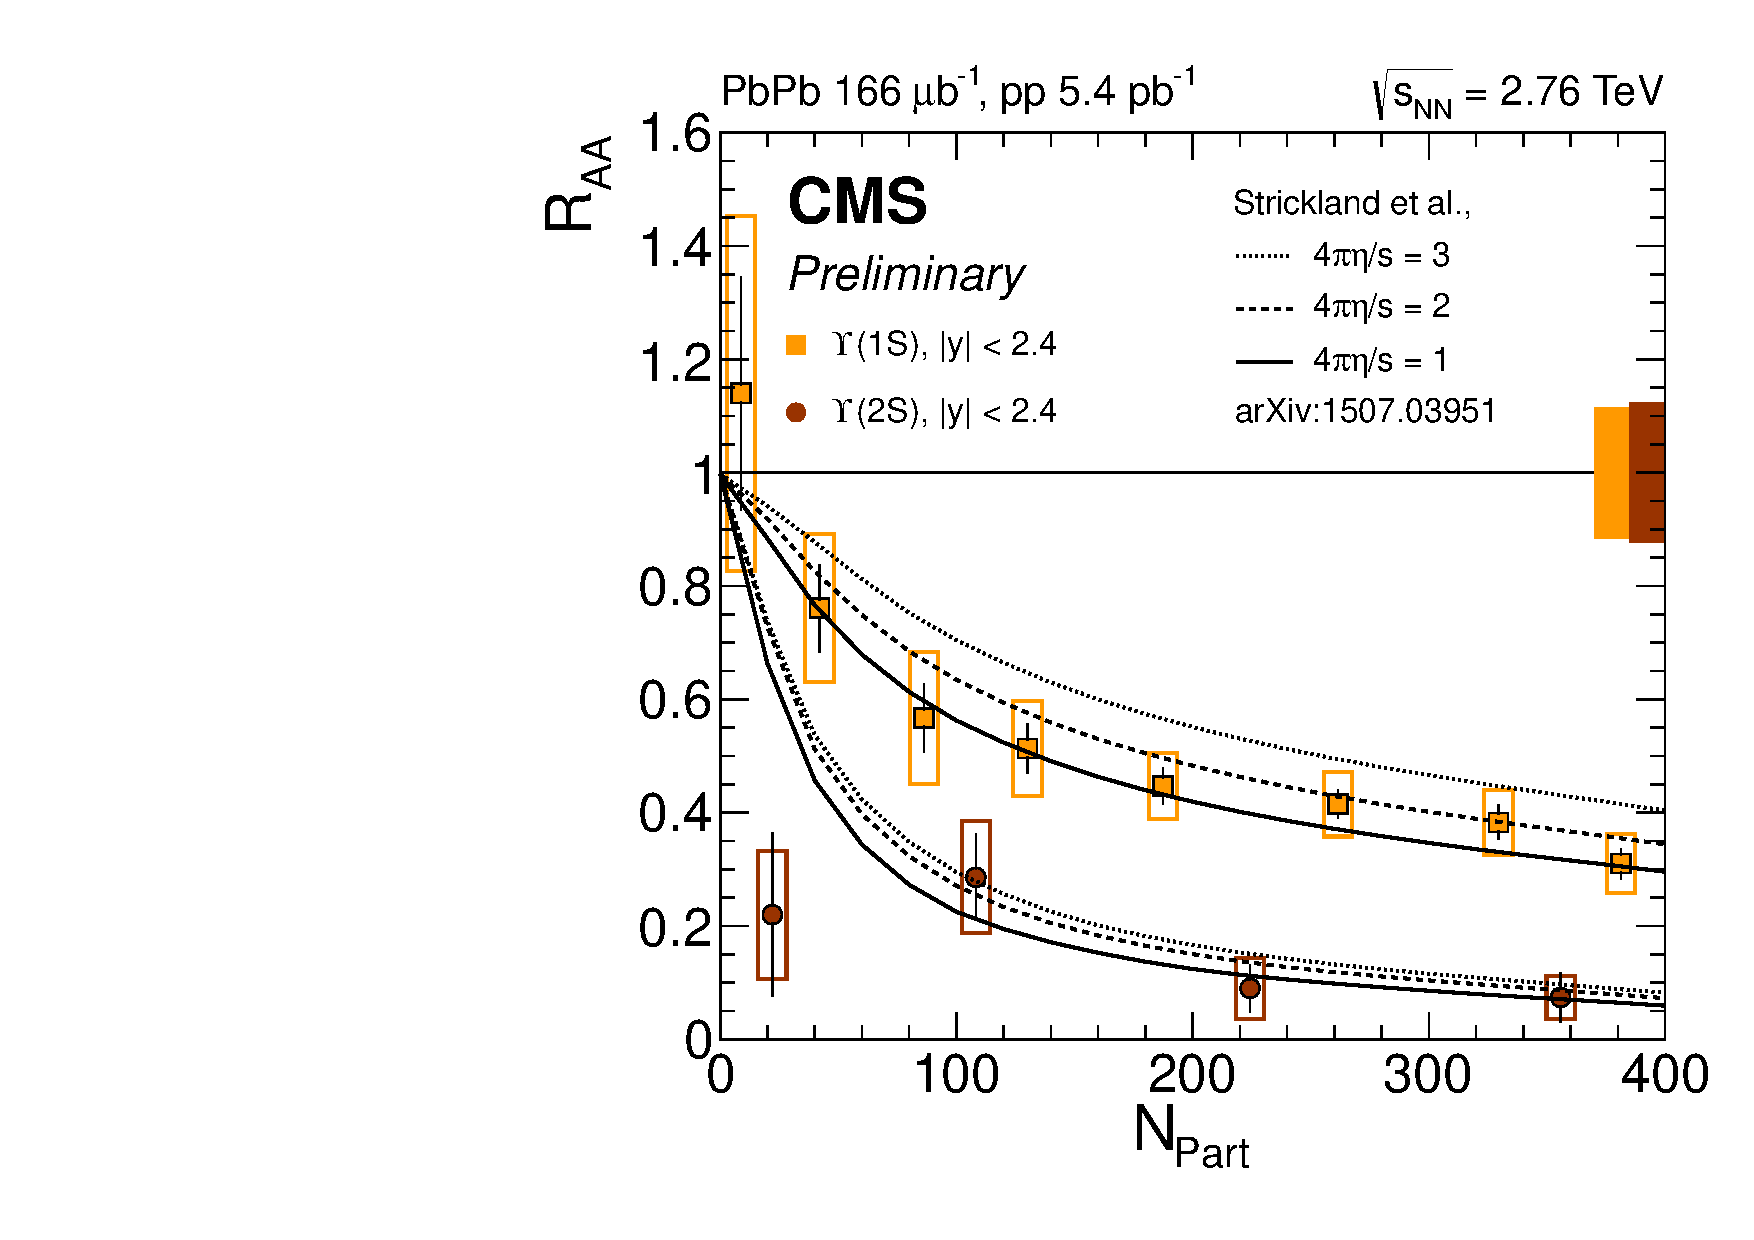
\includegraphics[width=0.465\textwidth]{Chapters/aUpsilon/RAA_NPART_Strickland.pdf}
%     \caption{PbPb nuclear modification factor \RAA\ in PbPb collisions
%     at \snn\ = 2.76 \TeV, as a function of the number of participants.}
%     \label{fig:RAA_npart}
%   \end{centering}  
% \end{figure}


% \subsection{Outlook}



% \subsection{Is \texorpdfstring{\PgUa}{Y(1S)} suppressed in PbPb collisions?}

% Following the analysis and the discussion of the \PgU\ state
% suppression in the PbPb

